\documentclass[twoside]{book}

% Packages required by doxygen
\usepackage{fixltx2e}
\usepackage{calc}
\usepackage{doxygen}
\usepackage[export]{adjustbox} % also loads graphicx
\usepackage{graphicx}
\usepackage[utf8]{inputenc}
\usepackage{makeidx}
\usepackage{multicol}
\usepackage{multirow}
\PassOptionsToPackage{warn}{textcomp}
\usepackage{textcomp}
\usepackage[nointegrals]{wasysym}
\usepackage[table]{xcolor}

% Font selection
\usepackage[T1]{fontenc}
\usepackage[scaled=.90]{helvet}
\usepackage{courier}
\usepackage{amssymb}
\usepackage{sectsty}
\renewcommand{\familydefault}{\sfdefault}
\allsectionsfont{%
  \fontseries{bc}\selectfont%
  \color{darkgray}%
}
\renewcommand{\DoxyLabelFont}{%
  \fontseries{bc}\selectfont%
  \color{darkgray}%
}
\newcommand{\+}{\discretionary{\mbox{\scriptsize$\hookleftarrow$}}{}{}}

% Page & text layout
\usepackage{geometry}
\geometry{%
  a4paper,%
  top=2.5cm,%
  bottom=2.5cm,%
  left=2.5cm,%
  right=2.5cm%
}
\tolerance=750
\hfuzz=15pt
\hbadness=750
\setlength{\emergencystretch}{15pt}
\setlength{\parindent}{0cm}
\setlength{\parskip}{0.2cm}
\makeatletter
\renewcommand{\paragraph}{%
  \@startsection{paragraph}{4}{0ex}{-1.0ex}{1.0ex}{%
    \normalfont\normalsize\bfseries\SS@parafont%
  }%
}
\renewcommand{\subparagraph}{%
  \@startsection{subparagraph}{5}{0ex}{-1.0ex}{1.0ex}{%
    \normalfont\normalsize\bfseries\SS@subparafont%
  }%
}
\makeatother

% Headers & footers
\usepackage{fancyhdr}
\pagestyle{fancyplain}
\fancyhead[LE]{\fancyplain{}{\bfseries\thepage}}
\fancyhead[CE]{\fancyplain{}{}}
\fancyhead[RE]{\fancyplain{}{\bfseries\leftmark}}
\fancyhead[LO]{\fancyplain{}{\bfseries\rightmark}}
\fancyhead[CO]{\fancyplain{}{}}
\fancyhead[RO]{\fancyplain{}{\bfseries\thepage}}
\fancyfoot[LE]{\fancyplain{}{}}
\fancyfoot[CE]{\fancyplain{}{}}
\fancyfoot[RE]{\fancyplain{}{\bfseries\scriptsize Generated on Fri May 15 2015 08\+:16\+:00 for Spexpert by Doxygen }}
\fancyfoot[LO]{\fancyplain{}{\bfseries\scriptsize Generated on Fri May 15 2015 08\+:16\+:00 for Spexpert by Doxygen }}
\fancyfoot[CO]{\fancyplain{}{}}
\fancyfoot[RO]{\fancyplain{}{}}
\renewcommand{\footrulewidth}{0.4pt}
\renewcommand{\chaptermark}[1]{%
  \markboth{#1}{}%
}
\renewcommand{\sectionmark}[1]{%
  \markright{\thesection\ #1}%
}

% Indices & bibliography
\usepackage{natbib}
\usepackage[titles]{tocloft}
\setcounter{tocdepth}{3}
\setcounter{secnumdepth}{5}
\makeindex

% Hyperlinks (required, but should be loaded last)
\usepackage{ifpdf}
\ifpdf
  \usepackage[pdftex,pagebackref=true]{hyperref}
\else
  \usepackage[ps2pdf,pagebackref=true]{hyperref}
\fi
\hypersetup{%
  colorlinks=true,%
  linkcolor=blue,%
  citecolor=blue,%
  unicode%
}

% Custom commands
\newcommand{\clearemptydoublepage}{%
  \newpage{\pagestyle{empty}\cleardoublepage}%
}


%===== C O N T E N T S =====

\begin{document}

% Titlepage & ToC
\hypersetup{pageanchor=false,
             bookmarks=true,
             bookmarksnumbered=true,
             pdfencoding=unicode
            }
\pagenumbering{roman}
\begin{titlepage}
\vspace*{7cm}
\begin{center}%
{\Large Spexpert }\\
\vspace*{1cm}
{\large Generated by Doxygen 1.8.9.1}\\
\vspace*{0.5cm}
{\small Fri May 15 2015 08:16:00}\\
\end{center}
\end{titlepage}
\clearemptydoublepage
\tableofcontents
\clearemptydoublepage
\pagenumbering{arabic}
\hypersetup{pageanchor=true}

%--- Begin generated contents ---
\chapter{Namespace Index}
\section{Namespace List}
Here is a list of all documented namespaces with brief descriptions\+:\begin{DoxyCompactList}
\item\contentsline{section}{\hyperlink{namespace_exp_task_list_traits}{Exp\+Task\+List\+Traits} \\*Contains \hyperlink{class_exp_task_list}{Exp\+Task\+List} traits }{\pageref{namespace_exp_task_list_traits}}{}
\item\contentsline{section}{\hyperlink{namespace_wait_task_list_traits}{Wait\+Task\+List\+Traits} \\*Namespace containing \hyperlink{class_wait_task_list}{Wait\+Task\+List}\textquotesingle{}s enums and helper structures }{\pageref{namespace_wait_task_list_traits}}{}
\end{DoxyCompactList}

\chapter{Hierarchical Index}
\section{Class Hierarchy}
This inheritance list is sorted roughly, but not completely, alphabetically\+:\begin{DoxyCompactList}
\item \contentsline{section}{Delayed\+Start}{\pageref{class_delayed_start}}{}
\item \contentsline{section}{Exp\+Task}{\pageref{class_exp_task}}{}
\begin{DoxyCompactList}
\item \contentsline{section}{Exp\+Task\+List}{\pageref{class_exp_task_list}}{}
\begin{DoxyCompactList}
\item \contentsline{section}{Wait\+Task\+List}{\pageref{class_wait_task_list}}{}
\end{DoxyCompactList}
\item \contentsline{section}{Fork\+Join\+Task}{\pageref{class_fork_join_task}}{}
\item \contentsline{section}{Wait\+Exp\+Task}{\pageref{class_wait_exp_task}}{}
\item \contentsline{section}{Waiting\+Task}{\pageref{class_waiting_task}}{}
\end{DoxyCompactList}
\item \contentsline{section}{Wait\+Task\+List\+Traits\+:\+:Task\+Item}{\pageref{struct_wait_task_list_traits_1_1_task_item}}{}
\item \contentsline{section}{Exp\+Task\+List\+Traits\+:\+:Task\+Item}{\pageref{struct_exp_task_list_traits_1_1_task_item}}{}
\item \contentsline{section}{Wait\+Task}{\pageref{class_wait_task}}{}
\item \contentsline{section}{Wait\+Worker}{\pageref{class_wait_worker}}{}
\end{DoxyCompactList}

\chapter{Data Structure Index}
\section{Data Structures}
Here are the data structures with brief descriptions\+:\begin{DoxyCompactList}
\item\contentsline{section}{\hyperlink{class_delayed_start}{Delayed\+Start} \\*This class is helper class, which wraps the \hyperlink{class_wait_task}{Wait\+Task} object if it has some \hyperlink{class_wait_task_a3984ae37eae1a984db2f2417df2bfbbf}{Wait\+Task\+::initial\+Delay()} in the Wait\+Worker\+::delayed\+Add\+Wait\+Task() method. Its method is invoked by a Q\+Timer after the initialy delay elapses. The \hyperlink{class_delayed_start_a579d849a61a9f20cb29bc18d5be7611a}{delayed\+Add\+Wait\+Task()} emits \hyperlink{class_delayed_start_ab12e84ab2900082373f556051f260c9c}{add\+Task()} signal, which is connected to the \hyperlink{class_wait_worker_a71dec4dbc5a123f20d0a5a7f707ed5a3}{Wait\+Worker\+::add\+Delayed\+Wait\+Task()} method and then it destroyes itself }{\pageref{class_delayed_start}}{}
\item\contentsline{section}{\hyperlink{class_exp_task}{Exp\+Task} \\*Abstract class, which forms the base for tasks usable with \hyperlink{class_exp_task_list}{Exp\+Task\+List} and \hyperlink{class_wait_task_list}{Wait\+Task\+List} }{\pageref{class_exp_task}}{}
\item\contentsline{section}{\hyperlink{class_exp_task_list}{Exp\+Task\+List} \\*\hyperlink{class_exp_task_list}{Exp\+Task\+List} }{\pageref{class_exp_task_list}}{}
\item\contentsline{section}{\hyperlink{class_fork_join_task}{Fork\+Join\+Task} \\*This class creates inside multiple \hyperlink{class_exp_task_list}{Exp\+Task\+List} objects and runs each of them in parallel when started, waiting for them all to finish }{\pageref{class_fork_join_task}}{}
\item\contentsline{section}{\hyperlink{struct_wait_task_list_traits_1_1_task_item}{Wait\+Task\+List\+Traits\+::\+Task\+Item} \\*Container for \hyperlink{class_wait_task}{Wait\+Task} attaching to it its type for faster runtime identification }{\pageref{struct_wait_task_list_traits_1_1_task_item}}{}
\item\contentsline{section}{\hyperlink{struct_exp_task_list_traits_1_1_task_item}{Exp\+Task\+List\+Traits\+::\+Task\+Item} \\*Container for \hyperlink{class_exp_task}{Exp\+Task} attaching to it its type for faster runtime identification }{\pageref{struct_exp_task_list_traits_1_1_task_item}}{}
\item\contentsline{section}{\hyperlink{class_wait_exp_task}{Wait\+Exp\+Task} \\*This class contains the \hyperlink{class_wait_task}{Wait\+Task} in the \hyperlink{struct_wait_task_list_traits_1_1_task_item}{Wait\+Task\+List\+Traits\+::\+Task\+Item}, which will be submited to the list of tasks which will be waited for, when added to the \hyperlink{class_wait_task_list}{Wait\+Task\+List}. Each \hyperlink{class_wait_task}{Wait\+Task} should be handled by some \hyperlink{class_waiting_task}{Waiting\+Task} to have some effect, so there shouldn\textquotesingle{}t be any \hyperlink{class_wait_exp_task}{Wait\+Exp\+Task} added to the \hyperlink{class_wait_task_list}{Wait\+Task\+List} without \hyperlink{class_waiting_task}{Waiting\+Task} added somewhere after it }{\pageref{class_wait_exp_task}}{}
\item\contentsline{section}{\hyperlink{class_waiting_task}{Waiting\+Task} \\*Handles waiting for all \hyperlink{class_wait_exp_task}{Wait\+Exp\+Task} objects previously added to the \hyperlink{class_wait_task_list}{Wait\+Task\+List} }{\pageref{class_waiting_task}}{}
\item\contentsline{section}{\hyperlink{class_wait_task}{Wait\+Task} \\*Abstract class which forms the base for task usable with \hyperlink{class_wait_task_list}{Wait\+Task\+List}. The \hyperlink{class_wait_task_a39f09592449c61469d093f980a23cbfd}{running()} method need to be reimplemented }{\pageref{class_wait_task}}{}
\item\contentsline{section}{\hyperlink{class_wait_task_list}{Wait\+Task\+List} \\*This class provides interface for executing tasks which waits for some process to be finished }{\pageref{class_wait_task_list}}{}
\item\contentsline{section}{\hyperlink{class_wait_worker}{Wait\+Worker} \\*This class is intended for the internal use in the \hyperlink{class_wait_task_list}{Wait\+Task\+List} for controlling if the processes controlled by \hyperlink{class_wait_task}{Wait\+Task} objects is running. It is executed in new thread }{\pageref{class_wait_worker}}{}
\end{DoxyCompactList}

\chapter{Namespace Documentation}
\hypertarget{namespace_exp_task_list_traits}{}\section{Exp\+Task\+List\+Traits Namespace Reference}
\label{namespace_exp_task_list_traits}\index{Exp\+Task\+List\+Traits@{Exp\+Task\+List\+Traits}}


Contains \hyperlink{class_exp_task_list}{Exp\+Task\+List} traits.  


\subsection*{Data Structures}
\begin{DoxyCompactItemize}
\item 
struct \hyperlink{struct_exp_task_list_traits_1_1_task_item}{Task\+Item}
\begin{DoxyCompactList}\small\item\em Container for \hyperlink{class_exp_task}{Exp\+Task} attaching to it its type for faster runtime identification. \end{DoxyCompactList}\end{DoxyCompactItemize}
\subsection*{Enumerations}
\begin{DoxyCompactItemize}
\item 
enum \hyperlink{namespace_exp_task_list_traits_adcf9a5159b43c6df6f5e6835170c25b2}{Task\+Type} \{ \\*
\hyperlink{namespace_exp_task_list_traits_adcf9a5159b43c6df6f5e6835170c25b2a6adf97f83acf6453d4a6a4b1070f3754}{Task\+Type\+::\+None}, 
\hyperlink{namespace_exp_task_list_traits_adcf9a5159b43c6df6f5e6835170c25b2a59aa4a0af2ecd23181fbb3244e6dfeb9}{Task\+Type\+::\+Exp\+List}, 
\hyperlink{namespace_exp_task_list_traits_adcf9a5159b43c6df6f5e6835170c25b2a671b5d94cee1d6950e5691b103a1e2a9}{Task\+Type\+::\+Wait\+List}, 
\hyperlink{namespace_exp_task_list_traits_adcf9a5159b43c6df6f5e6835170c25b2a1d0072304077daded3bc3d564dfa522a}{Task\+Type\+::\+Win\+Spec\+Start}, 
\\*
\hyperlink{namespace_exp_task_list_traits_adcf9a5159b43c6df6f5e6835170c25b2a9c65176b04994b682478d9804d988dff}{Task\+Type\+::\+Stage\+Control\+Run}, 
\hyperlink{namespace_exp_task_list_traits_adcf9a5159b43c6df6f5e6835170c25b2a2a058c6c07e8cadbfe7b8f834d30b21d}{Task\+Type\+::\+Stage\+Control\+To\+Limit}, 
\hyperlink{namespace_exp_task_list_traits_adcf9a5159b43c6df6f5e6835170c25b2a4e9c7414817cb40f524c8e9910159c03}{Task\+Type\+::\+Stage\+Control\+Send\+To\+Pos}, 
\hyperlink{namespace_exp_task_list_traits_adcf9a5159b43c6df6f5e6835170c25b2a42dd439086376f59b26899ac8da8a129}{Task\+Type\+::\+Stage\+Control\+Set\+Limit}, 
\\*
\hyperlink{namespace_exp_task_list_traits_adcf9a5159b43c6df6f5e6835170c25b2ab84553a63b9179867404478878a34c60}{Task\+Type\+::\+Stage\+Control\+Switch\+Power}, 
\hyperlink{namespace_exp_task_list_traits_adcf9a5159b43c6df6f5e6835170c25b2af03fc29c1c6475d88dd2302c439b05c4}{Task\+Type\+::\+Start\+Waiting}, 
\hyperlink{namespace_exp_task_list_traits_adcf9a5159b43c6df6f5e6835170c25b2aba7050260c96b48b8d46d6755cf193ea}{Task\+Type\+::\+Wait\+Exp}, 
\hyperlink{namespace_exp_task_list_traits_adcf9a5159b43c6df6f5e6835170c25b2a5706de961fb376d701be6e7762d8b09c}{Task\+Type\+::\+Waiting}
 \}
\begin{DoxyCompactList}\small\item\em This scoped enum contains the list of tasks for faster runtime identification. \end{DoxyCompactList}\end{DoxyCompactItemize}


\subsection{Detailed Description}
Contains \hyperlink{class_exp_task_list}{Exp\+Task\+List} traits. 

\subsection{Enumeration Type Documentation}
\hypertarget{namespace_exp_task_list_traits_adcf9a5159b43c6df6f5e6835170c25b2}{}\index{Exp\+Task\+List\+Traits@{Exp\+Task\+List\+Traits}!Task\+Type@{Task\+Type}}
\index{Task\+Type@{Task\+Type}!Exp\+Task\+List\+Traits@{Exp\+Task\+List\+Traits}}
\subsubsection[{Task\+Type}]{\setlength{\rightskip}{0pt plus 5cm}enum {\bf Exp\+Task\+List\+Traits\+::\+Task\+Type}\hspace{0.3cm}{\ttfamily [strong]}}\label{namespace_exp_task_list_traits_adcf9a5159b43c6df6f5e6835170c25b2}


This scoped enum contains the list of tasks for faster runtime identification. 

\begin{DoxySeeAlso}{See also}
\hyperlink{struct_exp_task_list_traits_1_1_task_item}{Task\+Item} 
\end{DoxySeeAlso}
\begin{Desc}
\item[Enumerator]\par
\begin{description}
\index{None@{None}!Exp\+Task\+List\+Traits@{Exp\+Task\+List\+Traits}}\index{Exp\+Task\+List\+Traits@{Exp\+Task\+List\+Traits}!None@{None}}\item[{\em 
\hypertarget{namespace_exp_task_list_traits_adcf9a5159b43c6df6f5e6835170c25b2a6adf97f83acf6453d4a6a4b1070f3754}{}None\label{namespace_exp_task_list_traits_adcf9a5159b43c6df6f5e6835170c25b2a6adf97f83acf6453d4a6a4b1070f3754}
}]none \index{Exp\+List@{Exp\+List}!Exp\+Task\+List\+Traits@{Exp\+Task\+List\+Traits}}\index{Exp\+Task\+List\+Traits@{Exp\+Task\+List\+Traits}!Exp\+List@{Exp\+List}}\item[{\em 
\hypertarget{namespace_exp_task_list_traits_adcf9a5159b43c6df6f5e6835170c25b2a59aa4a0af2ecd23181fbb3244e6dfeb9}{}Exp\+List\label{namespace_exp_task_list_traits_adcf9a5159b43c6df6f5e6835170c25b2a59aa4a0af2ecd23181fbb3244e6dfeb9}
}]\hyperlink{class_exp_task_list}{Exp\+Task\+List}. \index{Wait\+List@{Wait\+List}!Exp\+Task\+List\+Traits@{Exp\+Task\+List\+Traits}}\index{Exp\+Task\+List\+Traits@{Exp\+Task\+List\+Traits}!Wait\+List@{Wait\+List}}\item[{\em 
\hypertarget{namespace_exp_task_list_traits_adcf9a5159b43c6df6f5e6835170c25b2a671b5d94cee1d6950e5691b103a1e2a9}{}Wait\+List\label{namespace_exp_task_list_traits_adcf9a5159b43c6df6f5e6835170c25b2a671b5d94cee1d6950e5691b103a1e2a9}
}]\hyperlink{class_wait_task_list}{Wait\+Task\+List}. \index{Win\+Spec\+Start@{Win\+Spec\+Start}!Exp\+Task\+List\+Traits@{Exp\+Task\+List\+Traits}}\index{Exp\+Task\+List\+Traits@{Exp\+Task\+List\+Traits}!Win\+Spec\+Start@{Win\+Spec\+Start}}\item[{\em 
\hypertarget{namespace_exp_task_list_traits_adcf9a5159b43c6df6f5e6835170c25b2a1d0072304077daded3bc3d564dfa522a}{}Win\+Spec\+Start\label{namespace_exp_task_list_traits_adcf9a5159b43c6df6f5e6835170c25b2a1d0072304077daded3bc3d564dfa522a}
}]Win\+Spec\+Tasks\+::\+Start. \index{Stage\+Control\+Run@{Stage\+Control\+Run}!Exp\+Task\+List\+Traits@{Exp\+Task\+List\+Traits}}\index{Exp\+Task\+List\+Traits@{Exp\+Task\+List\+Traits}!Stage\+Control\+Run@{Stage\+Control\+Run}}\item[{\em 
\hypertarget{namespace_exp_task_list_traits_adcf9a5159b43c6df6f5e6835170c25b2a9c65176b04994b682478d9804d988dff}{}Stage\+Control\+Run\label{namespace_exp_task_list_traits_adcf9a5159b43c6df6f5e6835170c25b2a9c65176b04994b682478d9804d988dff}
}]Stage\+Tasks\+::\+Run. \index{Stage\+Control\+To\+Limit@{Stage\+Control\+To\+Limit}!Exp\+Task\+List\+Traits@{Exp\+Task\+List\+Traits}}\index{Exp\+Task\+List\+Traits@{Exp\+Task\+List\+Traits}!Stage\+Control\+To\+Limit@{Stage\+Control\+To\+Limit}}\item[{\em 
\hypertarget{namespace_exp_task_list_traits_adcf9a5159b43c6df6f5e6835170c25b2a2a058c6c07e8cadbfe7b8f834d30b21d}{}Stage\+Control\+To\+Limit\label{namespace_exp_task_list_traits_adcf9a5159b43c6df6f5e6835170c25b2a2a058c6c07e8cadbfe7b8f834d30b21d}
}]Stage\+Tasks\+::\+Go\+To\+Lim. \index{Stage\+Control\+Send\+To\+Pos@{Stage\+Control\+Send\+To\+Pos}!Exp\+Task\+List\+Traits@{Exp\+Task\+List\+Traits}}\index{Exp\+Task\+List\+Traits@{Exp\+Task\+List\+Traits}!Stage\+Control\+Send\+To\+Pos@{Stage\+Control\+Send\+To\+Pos}}\item[{\em 
\hypertarget{namespace_exp_task_list_traits_adcf9a5159b43c6df6f5e6835170c25b2a4e9c7414817cb40f524c8e9910159c03}{}Stage\+Control\+Send\+To\+Pos\label{namespace_exp_task_list_traits_adcf9a5159b43c6df6f5e6835170c25b2a4e9c7414817cb40f524c8e9910159c03}
}]Stage\+Tasks\+::\+Send\+To\+Pos. \index{Stage\+Control\+Set\+Limit@{Stage\+Control\+Set\+Limit}!Exp\+Task\+List\+Traits@{Exp\+Task\+List\+Traits}}\index{Exp\+Task\+List\+Traits@{Exp\+Task\+List\+Traits}!Stage\+Control\+Set\+Limit@{Stage\+Control\+Set\+Limit}}\item[{\em 
\hypertarget{namespace_exp_task_list_traits_adcf9a5159b43c6df6f5e6835170c25b2a42dd439086376f59b26899ac8da8a129}{}Stage\+Control\+Set\+Limit\label{namespace_exp_task_list_traits_adcf9a5159b43c6df6f5e6835170c25b2a42dd439086376f59b26899ac8da8a129}
}]Stage\+Tasks\+::\+Set\+Lim. \index{Stage\+Control\+Switch\+Power@{Stage\+Control\+Switch\+Power}!Exp\+Task\+List\+Traits@{Exp\+Task\+List\+Traits}}\index{Exp\+Task\+List\+Traits@{Exp\+Task\+List\+Traits}!Stage\+Control\+Switch\+Power@{Stage\+Control\+Switch\+Power}}\item[{\em 
\hypertarget{namespace_exp_task_list_traits_adcf9a5159b43c6df6f5e6835170c25b2ab84553a63b9179867404478878a34c60}{}Stage\+Control\+Switch\+Power\label{namespace_exp_task_list_traits_adcf9a5159b43c6df6f5e6835170c25b2ab84553a63b9179867404478878a34c60}
}]Stage\+Tasks\+::\+Switch\+Power. \index{Start\+Waiting@{Start\+Waiting}!Exp\+Task\+List\+Traits@{Exp\+Task\+List\+Traits}}\index{Exp\+Task\+List\+Traits@{Exp\+Task\+List\+Traits}!Start\+Waiting@{Start\+Waiting}}\item[{\em 
\hypertarget{namespace_exp_task_list_traits_adcf9a5159b43c6df6f5e6835170c25b2af03fc29c1c6475d88dd2302c439b05c4}{}Start\+Waiting\label{namespace_exp_task_list_traits_adcf9a5159b43c6df6f5e6835170c25b2af03fc29c1c6475d88dd2302c439b05c4}
}]Start\+Waiting\+Task. \index{Wait\+Exp@{Wait\+Exp}!Exp\+Task\+List\+Traits@{Exp\+Task\+List\+Traits}}\index{Exp\+Task\+List\+Traits@{Exp\+Task\+List\+Traits}!Wait\+Exp@{Wait\+Exp}}\item[{\em 
\hypertarget{namespace_exp_task_list_traits_adcf9a5159b43c6df6f5e6835170c25b2aba7050260c96b48b8d46d6755cf193ea}{}Wait\+Exp\label{namespace_exp_task_list_traits_adcf9a5159b43c6df6f5e6835170c25b2aba7050260c96b48b8d46d6755cf193ea}
}]\hyperlink{class_wait_exp_task}{Wait\+Exp\+Task}. \index{Waiting@{Waiting}!Exp\+Task\+List\+Traits@{Exp\+Task\+List\+Traits}}\index{Exp\+Task\+List\+Traits@{Exp\+Task\+List\+Traits}!Waiting@{Waiting}}\item[{\em 
\hypertarget{namespace_exp_task_list_traits_adcf9a5159b43c6df6f5e6835170c25b2a5706de961fb376d701be6e7762d8b09c}{}Waiting\label{namespace_exp_task_list_traits_adcf9a5159b43c6df6f5e6835170c25b2a5706de961fb376d701be6e7762d8b09c}
}]\hyperlink{class_waiting_task}{Waiting\+Task}. \end{description}
\end{Desc}

\hypertarget{namespace_wait_task_list_traits}{}\section{Wait\+Task\+List\+Traits Namespace Reference}
\label{namespace_wait_task_list_traits}\index{Wait\+Task\+List\+Traits@{Wait\+Task\+List\+Traits}}


Namespace containing \hyperlink{class_wait_task_list}{Wait\+Task\+List}\textquotesingle{}s enums and helper structures.  


\subsection*{Data Structures}
\begin{DoxyCompactItemize}
\item 
struct \hyperlink{struct_wait_task_list_traits_1_1_task_item}{Task\+Item}
\begin{DoxyCompactList}\small\item\em Container for \hyperlink{class_wait_task}{Wait\+Task} attaching to it its type for faster runtime identification. \end{DoxyCompactList}\end{DoxyCompactItemize}
\subsection*{Enumerations}
\begin{DoxyCompactItemize}
\item 
enum \hyperlink{namespace_wait_task_list_traits_a3cb74ee1929f03e51486087ef21caf9f}{Wait\+For} \+: unsigned char \{ \\*
\hyperlink{namespace_wait_task_list_traits_a3cb74ee1929f03e51486087ef21caf9fa6adf97f83acf6453d4a6a4b1070f3754}{Wait\+For\+::\+None} = 0, 
\hyperlink{namespace_wait_task_list_traits_a3cb74ee1929f03e51486087ef21caf9fa8f497c1a3d15af9e0c215019f26b887d}{Wait\+For\+::\+Delay} = 1 $<$$<$ 0, 
\hyperlink{namespace_wait_task_list_traits_a3cb74ee1929f03e51486087ef21caf9fa72be81983b1060a1c19315bfcc0fec96}{Wait\+For\+::\+Win\+Spec} = 1 $<$$<$ 1, 
\hyperlink{namespace_wait_task_list_traits_a3cb74ee1929f03e51486087ef21caf9fab33538179f5661a86cbe327a1793e199}{Wait\+For\+::\+Motor} = 1 $<$$<$ 2, 
\\*
\hyperlink{namespace_wait_task_list_traits_a3cb74ee1929f03e51486087ef21caf9fac7fc4af8d9e4c06e420a1396c67b2c05}{Wait\+For\+::\+Spectrograph} = 1 $<$$<$ 3, 
\hyperlink{namespace_wait_task_list_traits_a3cb74ee1929f03e51486087ef21caf9faed9aa33f81e5c861076f2b9a14cde0ce}{Wait\+For\+::\+Other1} = 1 $<$$<$ 4, 
\hyperlink{namespace_wait_task_list_traits_a3cb74ee1929f03e51486087ef21caf9fa73890f3ff21d36055971bc1837d1e378}{Wait\+For\+::\+Other2} = 1 $<$$<$ 5, 
\hyperlink{namespace_wait_task_list_traits_a3cb74ee1929f03e51486087ef21caf9fa9c5d1f216c477d66f934f6f2b626b472}{Wait\+For\+::\+Other3} = 1 $<$$<$ 6, 
\\*
\hyperlink{namespace_wait_task_list_traits_a3cb74ee1929f03e51486087ef21caf9fab5313789e3103b02c2c9a46d59e9c44e}{Wait\+For\+::\+Other4} = 1 $<$$<$ 7
 \}
\begin{DoxyCompactList}\small\item\em This scoped enum contains the list of tasks for faster runtime identification. \end{DoxyCompactList}\end{DoxyCompactItemize}
\subsection*{Functions}
\begin{DoxyCompactItemize}
\item 
\hypertarget{namespace_wait_task_list_traits_aa7a6bbfd5d35244e16c9368c6653370b}{}constexpr \hyperlink{namespace_wait_task_list_traits_a3cb74ee1929f03e51486087ef21caf9f}{Wait\+For} \hyperlink{namespace_wait_task_list_traits_aa7a6bbfd5d35244e16c9368c6653370b}{operator$\vert$} (\hyperlink{namespace_wait_task_list_traits_a3cb74ee1929f03e51486087ef21caf9f}{Wait\+For} a, \hyperlink{namespace_wait_task_list_traits_a3cb74ee1929f03e51486087ef21caf9f}{Wait\+For} b)\label{namespace_wait_task_list_traits_aa7a6bbfd5d35244e16c9368c6653370b}

\begin{DoxyCompactList}\small\item\em logical O\+R operator \end{DoxyCompactList}\item 
\hypertarget{namespace_wait_task_list_traits_a1db6fb338e8fb5ca6fcf85ac69aa6154}{}constexpr \hyperlink{namespace_wait_task_list_traits_a3cb74ee1929f03e51486087ef21caf9f}{Wait\+For} \hyperlink{namespace_wait_task_list_traits_a1db6fb338e8fb5ca6fcf85ac69aa6154}{operator\&} (\hyperlink{namespace_wait_task_list_traits_a3cb74ee1929f03e51486087ef21caf9f}{Wait\+For} a, \hyperlink{namespace_wait_task_list_traits_a3cb74ee1929f03e51486087ef21caf9f}{Wait\+For} b)\label{namespace_wait_task_list_traits_a1db6fb338e8fb5ca6fcf85ac69aa6154}

\begin{DoxyCompactList}\small\item\em logical A\+N\+D operator \end{DoxyCompactList}\item 
\hypertarget{namespace_wait_task_list_traits_aa82f582fbe230682bd2751a0caf0f238}{}\hyperlink{namespace_wait_task_list_traits_a3cb74ee1929f03e51486087ef21caf9f}{Wait\+For} \hyperlink{namespace_wait_task_list_traits_aa82f582fbe230682bd2751a0caf0f238}{operator$\sim$} (\hyperlink{namespace_wait_task_list_traits_a3cb74ee1929f03e51486087ef21caf9f}{Wait\+For} a)\label{namespace_wait_task_list_traits_aa82f582fbe230682bd2751a0caf0f238}

\begin{DoxyCompactList}\small\item\em logical negation operator \end{DoxyCompactList}\item 
\hypertarget{namespace_wait_task_list_traits_a3ace3b64b24680f2cdae3125b410c603}{}\hyperlink{namespace_wait_task_list_traits_a3cb74ee1929f03e51486087ef21caf9f}{Wait\+For} \& \hyperlink{namespace_wait_task_list_traits_a3ace3b64b24680f2cdae3125b410c603}{operator$\vert$=} (\hyperlink{namespace_wait_task_list_traits_a3cb74ee1929f03e51486087ef21caf9f}{Wait\+For} \&a, \hyperlink{namespace_wait_task_list_traits_a3cb74ee1929f03e51486087ef21caf9f}{Wait\+For} b)\label{namespace_wait_task_list_traits_a3ace3b64b24680f2cdae3125b410c603}

\begin{DoxyCompactList}\small\item\em logical assignment O\+R operator \end{DoxyCompactList}\item 
\hypertarget{namespace_wait_task_list_traits_a548dc243d47ac061fed8d9bbcda095b7}{}\hyperlink{namespace_wait_task_list_traits_a3cb74ee1929f03e51486087ef21caf9f}{Wait\+For} \& \hyperlink{namespace_wait_task_list_traits_a548dc243d47ac061fed8d9bbcda095b7}{operator\&=} (\hyperlink{namespace_wait_task_list_traits_a3cb74ee1929f03e51486087ef21caf9f}{Wait\+For} \&a, \hyperlink{namespace_wait_task_list_traits_a3cb74ee1929f03e51486087ef21caf9f}{Wait\+For} b)\label{namespace_wait_task_list_traits_a548dc243d47ac061fed8d9bbcda095b7}

\begin{DoxyCompactList}\small\item\em logical assignment A\+N\+D operator \end{DoxyCompactList}\end{DoxyCompactItemize}


\subsection{Detailed Description}
Namespace containing \hyperlink{class_wait_task_list}{Wait\+Task\+List}\textquotesingle{}s enums and helper structures. 

\subsection{Enumeration Type Documentation}
\hypertarget{namespace_wait_task_list_traits_a3cb74ee1929f03e51486087ef21caf9f}{}\index{Wait\+Task\+List\+Traits@{Wait\+Task\+List\+Traits}!Wait\+For@{Wait\+For}}
\index{Wait\+For@{Wait\+For}!Wait\+Task\+List\+Traits@{Wait\+Task\+List\+Traits}}
\subsubsection[{Wait\+For}]{\setlength{\rightskip}{0pt plus 5cm}enum {\bf Wait\+Task\+List\+Traits\+::\+Wait\+For} \+: unsigned char\hspace{0.3cm}{\ttfamily [strong]}}\label{namespace_wait_task_list_traits_a3cb74ee1929f03e51486087ef21caf9f}


This scoped enum contains the list of tasks for faster runtime identification. 

\begin{DoxySeeAlso}{See also}
\hyperlink{struct_wait_task_list_traits_1_1_task_item}{Task\+Item} 
\end{DoxySeeAlso}
\begin{Desc}
\item[Enumerator]\par
\begin{description}
\index{None@{None}!Wait\+Task\+List\+Traits@{Wait\+Task\+List\+Traits}}\index{Wait\+Task\+List\+Traits@{Wait\+Task\+List\+Traits}!None@{None}}\item[{\em 
\hypertarget{namespace_wait_task_list_traits_a3cb74ee1929f03e51486087ef21caf9fa6adf97f83acf6453d4a6a4b1070f3754}{}None\label{namespace_wait_task_list_traits_a3cb74ee1929f03e51486087ef21caf9fa6adf97f83acf6453d4a6a4b1070f3754}
}]None. \index{Delay@{Delay}!Wait\+Task\+List\+Traits@{Wait\+Task\+List\+Traits}}\index{Wait\+Task\+List\+Traits@{Wait\+Task\+List\+Traits}!Delay@{Delay}}\item[{\em 
\hypertarget{namespace_wait_task_list_traits_a3cb74ee1929f03e51486087ef21caf9fa8f497c1a3d15af9e0c215019f26b887d}{}Delay\label{namespace_wait_task_list_traits_a3cb74ee1929f03e51486087ef21caf9fa8f497c1a3d15af9e0c215019f26b887d}
}]Delay\+Wait\+Task. \index{Win\+Spec@{Win\+Spec}!Wait\+Task\+List\+Traits@{Wait\+Task\+List\+Traits}}\index{Wait\+Task\+List\+Traits@{Wait\+Task\+List\+Traits}!Win\+Spec@{Win\+Spec}}\item[{\em 
\hypertarget{namespace_wait_task_list_traits_a3cb74ee1929f03e51486087ef21caf9fa72be81983b1060a1c19315bfcc0fec96}{}Win\+Spec\label{namespace_wait_task_list_traits_a3cb74ee1929f03e51486087ef21caf9fa72be81983b1060a1c19315bfcc0fec96}
}]Win\+Spec\+Wait\+Task. \index{Motor@{Motor}!Wait\+Task\+List\+Traits@{Wait\+Task\+List\+Traits}}\index{Wait\+Task\+List\+Traits@{Wait\+Task\+List\+Traits}!Motor@{Motor}}\item[{\em 
\hypertarget{namespace_wait_task_list_traits_a3cb74ee1929f03e51486087ef21caf9fab33538179f5661a86cbe327a1793e199}{}Motor\label{namespace_wait_task_list_traits_a3cb74ee1929f03e51486087ef21caf9fab33538179f5661a86cbe327a1793e199}
}]Stage\+Control\+Wait\+Task. \index{Spectrograph@{Spectrograph}!Wait\+Task\+List\+Traits@{Wait\+Task\+List\+Traits}}\index{Wait\+Task\+List\+Traits@{Wait\+Task\+List\+Traits}!Spectrograph@{Spectrograph}}\item[{\em 
\hypertarget{namespace_wait_task_list_traits_a3cb74ee1929f03e51486087ef21caf9fac7fc4af8d9e4c06e420a1396c67b2c05}{}Spectrograph\label{namespace_wait_task_list_traits_a3cb74ee1929f03e51486087ef21caf9fac7fc4af8d9e4c06e420a1396c67b2c05}
}]for future use \index{Other1@{Other1}!Wait\+Task\+List\+Traits@{Wait\+Task\+List\+Traits}}\index{Wait\+Task\+List\+Traits@{Wait\+Task\+List\+Traits}!Other1@{Other1}}\item[{\em 
\hypertarget{namespace_wait_task_list_traits_a3cb74ee1929f03e51486087ef21caf9faed9aa33f81e5c861076f2b9a14cde0ce}{}Other1\label{namespace_wait_task_list_traits_a3cb74ee1929f03e51486087ef21caf9faed9aa33f81e5c861076f2b9a14cde0ce}
}]for future use \index{Other2@{Other2}!Wait\+Task\+List\+Traits@{Wait\+Task\+List\+Traits}}\index{Wait\+Task\+List\+Traits@{Wait\+Task\+List\+Traits}!Other2@{Other2}}\item[{\em 
\hypertarget{namespace_wait_task_list_traits_a3cb74ee1929f03e51486087ef21caf9fa73890f3ff21d36055971bc1837d1e378}{}Other2\label{namespace_wait_task_list_traits_a3cb74ee1929f03e51486087ef21caf9fa73890f3ff21d36055971bc1837d1e378}
}]for future use \index{Other3@{Other3}!Wait\+Task\+List\+Traits@{Wait\+Task\+List\+Traits}}\index{Wait\+Task\+List\+Traits@{Wait\+Task\+List\+Traits}!Other3@{Other3}}\item[{\em 
\hypertarget{namespace_wait_task_list_traits_a3cb74ee1929f03e51486087ef21caf9fa9c5d1f216c477d66f934f6f2b626b472}{}Other3\label{namespace_wait_task_list_traits_a3cb74ee1929f03e51486087ef21caf9fa9c5d1f216c477d66f934f6f2b626b472}
}]for future use \index{Other4@{Other4}!Wait\+Task\+List\+Traits@{Wait\+Task\+List\+Traits}}\index{Wait\+Task\+List\+Traits@{Wait\+Task\+List\+Traits}!Other4@{Other4}}\item[{\em 
\hypertarget{namespace_wait_task_list_traits_a3cb74ee1929f03e51486087ef21caf9fab5313789e3103b02c2c9a46d59e9c44e}{}Other4\label{namespace_wait_task_list_traits_a3cb74ee1929f03e51486087ef21caf9fab5313789e3103b02c2c9a46d59e9c44e}
}]for future use \end{description}
\end{Desc}

\chapter{Data Structure Documentation}
\hypertarget{class_delayed_start}{}\section{Delayed\+Start Class Reference}
\label{class_delayed_start}\index{Delayed\+Start@{Delayed\+Start}}


This class is helper class, which wraps the \hyperlink{class_wait_task}{Wait\+Task} object if it has some \hyperlink{class_wait_task_a3984ae37eae1a984db2f2417df2bfbbf}{Wait\+Task\+::initial\+Delay()} in the Wait\+Worker\+::delayed\+Add\+Wait\+Task() method. Its method is invoked by a Q\+Timer after the initialy delay elapses. The \hyperlink{class_delayed_start_a579d849a61a9f20cb29bc18d5be7611a}{delayed\+Add\+Wait\+Task()} emits \hyperlink{class_delayed_start_ab12e84ab2900082373f556051f260c9c}{add\+Task()} signal, which is connected to the \hyperlink{class_wait_worker_a71dec4dbc5a123f20d0a5a7f707ed5a3}{Wait\+Worker\+::add\+Delayed\+Wait\+Task()} method and then it destroyes itself.  




Inherits Q\+Object.

\subsection*{Public Slots}
\begin{DoxyCompactItemize}
\item 
\hypertarget{class_delayed_start_a579d849a61a9f20cb29bc18d5be7611a}{}void \hyperlink{class_delayed_start_a579d849a61a9f20cb29bc18d5be7611a}{delayed\+Add\+Wait\+Task} ()\label{class_delayed_start_a579d849a61a9f20cb29bc18d5be7611a}

\begin{DoxyCompactList}\small\item\em This slot is invoked by the Q\+Timer from the \hyperlink{class_wait_worker_adaff9ea88795fa9d902711c1952828cd}{Wait\+Worker\+::add\+Wait\+Task()} method. It emits \hyperlink{class_delayed_start_ab12e84ab2900082373f556051f260c9c}{add\+Task()} signal and deletes the \hyperlink{class_delayed_start}{Delayed\+Start} object. \end{DoxyCompactList}\end{DoxyCompactItemize}
\subsection*{Signals}
\begin{DoxyCompactItemize}
\item 
\hypertarget{class_delayed_start_ab12e84ab2900082373f556051f260c9c}{}void \hyperlink{class_delayed_start_ab12e84ab2900082373f556051f260c9c}{add\+Task} (\hyperlink{struct_wait_task_list_traits_1_1_task_item}{Wait\+Task\+List\+Traits\+::\+Task\+Item} wait\+Task\+Item)\label{class_delayed_start_ab12e84ab2900082373f556051f260c9c}

\begin{DoxyCompactList}\small\item\em This signal is emited from the \hyperlink{class_delayed_start_a579d849a61a9f20cb29bc18d5be7611a}{delayed\+Add\+Wait\+Task()} method and connected to the \hyperlink{class_wait_worker_a71dec4dbc5a123f20d0a5a7f707ed5a3}{Wait\+Worker\+::add\+Delayed\+Wait\+Task()} slot. \end{DoxyCompactList}\end{DoxyCompactItemize}
\subsection*{Public Member Functions}
\begin{DoxyCompactItemize}
\item 
\hyperlink{class_delayed_start_a68f9a781f7423106276e4a1f1e169fed}{Delayed\+Start} (const \hyperlink{struct_wait_task_list_traits_1_1_task_item}{Wait\+Task\+List\+Traits\+::\+Task\+Item} \&wait\+Task\+Item, Q\+Object $\ast$parent=0)
\begin{DoxyCompactList}\small\item\em Constructs the \hyperlink{class_delayed_start}{Delayed\+Start} object. \end{DoxyCompactList}\item 
\hypertarget{class_delayed_start_aa0e567f544ba762575a7ff045a9864ea}{}\hyperlink{class_delayed_start_aa0e567f544ba762575a7ff045a9864ea}{$\sim$\+Delayed\+Start} ()\label{class_delayed_start_aa0e567f544ba762575a7ff045a9864ea}

\begin{DoxyCompactList}\small\item\em Destroyes \hyperlink{class_delayed_start}{Delayed\+Start} objects. \end{DoxyCompactList}\end{DoxyCompactItemize}
\subsection*{Private Attributes}
\begin{DoxyCompactItemize}
\item 
\hypertarget{class_delayed_start_ad6297f6dba9b4b767486e7a732d4e238}{}\hyperlink{struct_wait_task_list_traits_1_1_task_item}{Wait\+Task\+List\+Traits\+::\+Task\+Item} \hyperlink{class_delayed_start_ad6297f6dba9b4b767486e7a732d4e238}{wait\+Task\+Item\+\_\+}\label{class_delayed_start_ad6297f6dba9b4b767486e7a732d4e238}

\begin{DoxyCompactList}\small\item\em contained \hyperlink{class_wait_task}{Wait\+Task}. \end{DoxyCompactList}\end{DoxyCompactItemize}


\subsection{Detailed Description}
This class is helper class, which wraps the \hyperlink{class_wait_task}{Wait\+Task} object if it has some \hyperlink{class_wait_task_a3984ae37eae1a984db2f2417df2bfbbf}{Wait\+Task\+::initial\+Delay()} in the Wait\+Worker\+::delayed\+Add\+Wait\+Task() method. Its method is invoked by a Q\+Timer after the initialy delay elapses. The \hyperlink{class_delayed_start_a579d849a61a9f20cb29bc18d5be7611a}{delayed\+Add\+Wait\+Task()} emits \hyperlink{class_delayed_start_ab12e84ab2900082373f556051f260c9c}{add\+Task()} signal, which is connected to the \hyperlink{class_wait_worker_a71dec4dbc5a123f20d0a5a7f707ed5a3}{Wait\+Worker\+::add\+Delayed\+Wait\+Task()} method and then it destroyes itself. 

\subsection{Constructor \& Destructor Documentation}
\hypertarget{class_delayed_start_a68f9a781f7423106276e4a1f1e169fed}{}\index{Delayed\+Start@{Delayed\+Start}!Delayed\+Start@{Delayed\+Start}}
\index{Delayed\+Start@{Delayed\+Start}!Delayed\+Start@{Delayed\+Start}}
\subsubsection[{Delayed\+Start}]{\setlength{\rightskip}{0pt plus 5cm}Delayed\+Start\+::\+Delayed\+Start (
\begin{DoxyParamCaption}
\item[{const {\bf Wait\+Task\+List\+Traits\+::\+Task\+Item} \&}]{wait\+Task\+Item, }
\item[{Q\+Object $\ast$}]{parent = {\ttfamily 0}}
\end{DoxyParamCaption}
)}\label{class_delayed_start_a68f9a781f7423106276e4a1f1e169fed}


Constructs the \hyperlink{class_delayed_start}{Delayed\+Start} object. 


\begin{DoxyParams}{Parameters}
{\em wait\+Task\+Item} & The \hyperlink{class_wait_task}{Wait\+Task}, which may be delayed. \\
\hline
{\em parent} & A parent in the Qt\textquotesingle{}s ownership system. \\
\hline
\end{DoxyParams}


The documentation for this class was generated from the following files\+:\begin{DoxyCompactItemize}
\item 
waittasklist.\+h\item 
waittasklist.\+cpp\end{DoxyCompactItemize}

\hypertarget{class_exp_task}{}\section{Exp\+Task Class Reference}
\label{class_exp_task}\index{Exp\+Task@{Exp\+Task}}


Abstract class, which forms the base for tasks usable with \hyperlink{class_exp_task_list}{Exp\+Task\+List} and \hyperlink{class_wait_task_list}{Wait\+Task\+List}.  




Inheritance diagram for Exp\+Task\+:\nopagebreak
\begin{figure}[H]
\begin{center}
\leavevmode
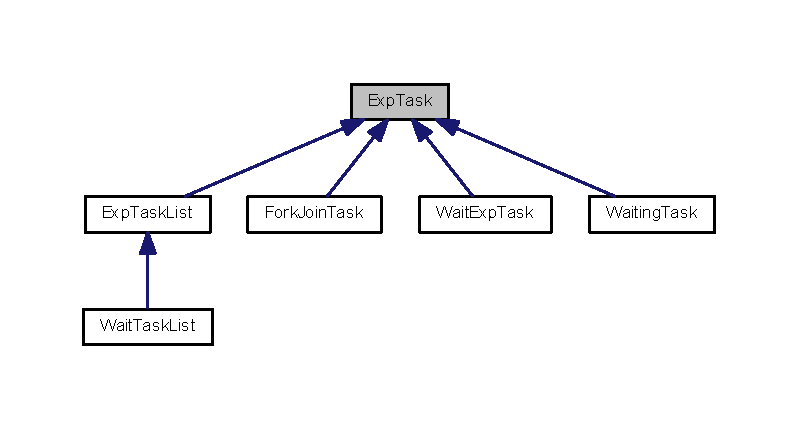
\includegraphics[width=350pt]{class_exp_task__inherit__graph}
\end{center}
\end{figure}
\subsection*{Public Slots}
\begin{DoxyCompactItemize}
\item 
\hypertarget{class_exp_task_a58da730e303ed8dee404b9420e4099f3}{}virtual void \hyperlink{class_exp_task_a58da730e303ed8dee404b9420e4099f3}{start} ()=0\label{class_exp_task_a58da730e303ed8dee404b9420e4099f3}

\begin{DoxyCompactList}\small\item\em pure virtual method, need to be reimplemented \end{DoxyCompactList}\item 
\hypertarget{class_exp_task_a22f581786f11fa3c7dc52ff90c6b7043}{}virtual void \hyperlink{class_exp_task_a22f581786f11fa3c7dc52ff90c6b7043}{stop} ()\label{class_exp_task_a22f581786f11fa3c7dc52ff90c6b7043}

\begin{DoxyCompactList}\small\item\em stops the execution of the task emiting \hyperlink{class_exp_task_a1a766503f6eb22b82c6e31e279b0ea9d}{task\+Failed()} and \hyperlink{class_exp_task_aeb51d072a7b96f55da3738a8c7733611}{finished()} signals. \end{DoxyCompactList}\end{DoxyCompactItemize}
\subsection*{Signals}
\begin{DoxyCompactItemize}
\item 
\hypertarget{class_exp_task_aeb51d072a7b96f55da3738a8c7733611}{}void \hyperlink{class_exp_task_aeb51d072a7b96f55da3738a8c7733611}{finished} ()\label{class_exp_task_aeb51d072a7b96f55da3738a8c7733611}

\begin{DoxyCompactList}\small\item\em signal emited when the task execution is finished \end{DoxyCompactList}\item 
\hypertarget{class_exp_task_a1a766503f6eb22b82c6e31e279b0ea9d}{}void \hyperlink{class_exp_task_a1a766503f6eb22b82c6e31e279b0ea9d}{task\+Failed} ()\label{class_exp_task_a1a766503f6eb22b82c6e31e279b0ea9d}

\begin{DoxyCompactList}\small\item\em emited when task execution failed, for example when the execution is interupted by the execution of \hyperlink{class_exp_task_a22f581786f11fa3c7dc52ff90c6b7043}{stop()} slot. \end{DoxyCompactList}\end{DoxyCompactItemize}
\subsection*{Public Member Functions}
\begin{DoxyCompactItemize}
\item 
\hyperlink{class_exp_task_ab741ec0a236695211f2b772881ae756c}{Exp\+Task} (Q\+Object $\ast$parent=0)
\begin{DoxyCompactList}\small\item\em Construct the \hyperlink{class_exp_task}{Exp\+Task} object. \end{DoxyCompactList}\item 
\hypertarget{class_exp_task_a069cc9e82376256ef25b76d19f881901}{}virtual \hyperlink{class_exp_task_a069cc9e82376256ef25b76d19f881901}{$\sim$\+Exp\+Task} ()\label{class_exp_task_a069cc9e82376256ef25b76d19f881901}

\begin{DoxyCompactList}\small\item\em empty destructor. \end{DoxyCompactList}\item 
void \hyperlink{class_exp_task_a4b1e37a956ea18764bb62b8b9ffa52d3}{once\+Executed} ()
\begin{DoxyCompactList}\small\item\em This method lowers execution counter \hyperlink{class_exp_task_a56421ba6834b53d845c1c6d14ede077f}{Exp\+Task\+::curr\+Times\+Exec\+\_\+}, which controls a number of repetitions the \hyperlink{class_exp_task}{Exp\+Task} was executed. \end{DoxyCompactList}\item 
virtual void \hyperlink{class_exp_task_ac84290f4ee014237657794522350cfea}{restart\+Times\+Exec} ()
\begin{DoxyCompactList}\small\item\em This method resets the current execution number counter \hyperlink{class_exp_task_a56421ba6834b53d845c1c6d14ede077f}{Exp\+Task\+::curr\+Times\+Exec\+\_\+} to the initial number of executions \hyperlink{class_exp_task_af38ca6f3252632f98e496758349477ac}{Exp\+Task\+::times\+Exec\+\_\+}. \end{DoxyCompactList}\item 
int \hyperlink{class_exp_task_a1ab988b6d9eb6d61cd1b3ac1a1c42153}{curr\+Times\+Exec} () const 
\begin{DoxyCompactList}\small\item\em This method gets current number of executions to be executed stored in the \hyperlink{class_exp_task_a56421ba6834b53d845c1c6d14ede077f}{Exp\+Task\+::curr\+Times\+Exec\+\_\+} variable. \end{DoxyCompactList}\item 
int \hyperlink{class_exp_task_acdb19df2cfecd5c7f7d28141b062a6fe}{times\+Exec} () const 
\begin{DoxyCompactList}\small\item\em This method gets the initial number of repetitions stored in the \hyperlink{class_exp_task_af38ca6f3252632f98e496758349477ac}{Exp\+Task\+::times\+Exec\+\_\+} variable. \end{DoxyCompactList}\item 
bool \hyperlink{class_exp_task_a440f37ee2170c077082f3d29f229be1b}{delayed\+Delete} () const 
\begin{DoxyCompactList}\small\item\em This method returns true if the \hyperlink{class_exp_task}{Exp\+Task} object could not be deleted after the number of executions \hyperlink{class_exp_task_a1ab988b6d9eb6d61cd1b3ac1a1c42153}{curr\+Times\+Exec()} reaches zero. \end{DoxyCompactList}\item 
void \hyperlink{class_exp_task_a9de0c990109370dea83ca471a05e1772}{set\+Times\+Exec} (int times\+Executed)
\begin{DoxyCompactList}\small\item\em This method sets the initial number of repetitions of the \hyperlink{class_exp_task}{Exp\+Task}. \end{DoxyCompactList}\item 
virtual void \hyperlink{class_exp_task_a2049ca37582a4b3250f3fc46ba19fe2a}{set\+Delayed\+Delete} (bool bl\+Delayed\+Delete)
\begin{DoxyCompactList}\small\item\em This method marks the \hyperlink{class_exp_task}{Exp\+Task} delayed delete. If it is set to true, the \hyperlink{class_exp_task}{Exp\+Task} object could not be dleted after the number of executions \hyperlink{class_exp_task_a1ab988b6d9eb6d61cd1b3ac1a1c42153}{curr\+Times\+Exec()} reaches zero (typically because it is a part of the a chain of more exptasks which may be exetuted more times as whole). \end{DoxyCompactList}\end{DoxyCompactItemize}
\subsection*{Private Attributes}
\begin{DoxyCompactItemize}
\item 
\hypertarget{class_exp_task_af38ca6f3252632f98e496758349477ac}{}int \hyperlink{class_exp_task_af38ca6f3252632f98e496758349477ac}{times\+Exec\+\_\+}\label{class_exp_task_af38ca6f3252632f98e496758349477ac}

\begin{DoxyCompactList}\small\item\em A variable which denotes how many times the task is executed when inserted in the \hyperlink{class_exp_task_list}{Exp\+Task\+List}. This variable is set by the \hyperlink{class_exp_task_a9de0c990109370dea83ca471a05e1772}{set\+Times\+Exec()} and get by the \hyperlink{class_exp_task_acdb19df2cfecd5c7f7d28141b062a6fe}{times\+Exec()}methods. The current remaining number of executions is stored in \hyperlink{class_exp_task_a56421ba6834b53d845c1c6d14ede077f}{Exp\+Task\+::curr\+Times\+Exec\+\_\+}, which can be reset to the \hyperlink{class_exp_task_af38ca6f3252632f98e496758349477ac}{Exp\+Task\+::times\+Exec\+\_\+} by the \hyperlink{class_exp_task_ac84290f4ee014237657794522350cfea}{restart\+Times\+Exec()} method. \end{DoxyCompactList}\item 
\hypertarget{class_exp_task_a56421ba6834b53d845c1c6d14ede077f}{}int \hyperlink{class_exp_task_a56421ba6834b53d845c1c6d14ede077f}{curr\+Times\+Exec\+\_\+}\label{class_exp_task_a56421ba6834b53d845c1c6d14ede077f}

\begin{DoxyCompactList}\small\item\em A variable which denotes how many executions of the task remain when inserted in the \hyperlink{class_exp_task_list}{Exp\+Task\+List}. It can be decremented by the once\+Executed method and reset to the \hyperlink{class_exp_task_af38ca6f3252632f98e496758349477ac}{Exp\+Task\+::times\+Exec\+\_\+} value by the \hyperlink{class_exp_task_ac84290f4ee014237657794522350cfea}{restart\+Times\+Exec()} method. The value of this variable can be obtained by the \hyperlink{class_exp_task_a1ab988b6d9eb6d61cd1b3ac1a1c42153}{curr\+Times\+Exec()} method. \end{DoxyCompactList}\item 
\hypertarget{class_exp_task_a9771cd4fb35fe809474e68810f66759c}{}bool \hyperlink{class_exp_task_a9771cd4fb35fe809474e68810f66759c}{bl\+Delayed\+Delete\+\_\+}\label{class_exp_task_a9771cd4fb35fe809474e68810f66759c}

\begin{DoxyCompactList}\small\item\em This variable indicates wheather the task should be deleted later (when it is part of some execution chain, which may be executed more than one times) or directly after the \hyperlink{class_exp_task_acdb19df2cfecd5c7f7d28141b062a6fe}{times\+Exec()} reaches zero. It can be obtained by the \hyperlink{class_exp_task_a440f37ee2170c077082f3d29f229be1b}{delayed\+Delete()} and set by \hyperlink{class_exp_task_a2049ca37582a4b3250f3fc46ba19fe2a}{set\+Delayed\+Delete()} method. \end{DoxyCompactList}\end{DoxyCompactItemize}


\subsection{Detailed Description}
Abstract class, which forms the base for tasks usable with \hyperlink{class_exp_task_list}{Exp\+Task\+List} and \hyperlink{class_wait_task_list}{Wait\+Task\+List}. 

The task stores the number of repetitions of this task to be executed, which can be set by the \hyperlink{class_exp_task_a9de0c990109370dea83ca471a05e1772}{set\+Times\+Exec()} method. Each finished execution requires the \hyperlink{class_exp_task_a4b1e37a956ea18764bb62b8b9ffa52d3}{once\+Executed()} method to be called. Spare execution repetitions can be obtained by the \hyperlink{class_exp_task_a1ab988b6d9eb6d61cd1b3ac1a1c42153}{curr\+Times\+Exec()} method and the counter of current spare executions can be reset to the initial value by the \hyperlink{class_exp_task_ac84290f4ee014237657794522350cfea}{restart\+Times\+Exec()} method.

The \hyperlink{class_exp_task}{Exp\+Task} can be marked not to be deleted immediatelly after the execution counter reaches zero by the \hyperlink{class_exp_task_a2049ca37582a4b3250f3fc46ba19fe2a}{set\+Delayed\+Delete()} method. This is useful if the task is part of some \hyperlink{class_exp_task}{Exp\+Task} chain (for example \hyperlink{class_exp_task_list}{Exp\+Task\+List}) which is set to be executed more times, so the task is stored for the next execution of the whole list. If the task is marked to be deleted later can be obtained by the \hyperlink{class_exp_task_a440f37ee2170c077082f3d29f229be1b}{delayed\+Delete()} method. 

\subsection{Constructor \& Destructor Documentation}
\hypertarget{class_exp_task_ab741ec0a236695211f2b772881ae756c}{}\index{Exp\+Task@{Exp\+Task}!Exp\+Task@{Exp\+Task}}
\index{Exp\+Task@{Exp\+Task}!Exp\+Task@{Exp\+Task}}
\subsubsection[{Exp\+Task}]{\setlength{\rightskip}{0pt plus 5cm}Exp\+Task\+::\+Exp\+Task (
\begin{DoxyParamCaption}
\item[{Q\+Object $\ast$}]{parent = {\ttfamily 0}}
\end{DoxyParamCaption}
)\hspace{0.3cm}{\ttfamily [explicit]}}\label{class_exp_task_ab741ec0a236695211f2b772881ae756c}


Construct the \hyperlink{class_exp_task}{Exp\+Task} object. 


\begin{DoxyParams}{Parameters}
{\em parent} & A parent Q\+Object in Qt\textquotesingle{}s ownership system. \\
\hline
\end{DoxyParams}


\subsection{Member Function Documentation}
\hypertarget{class_exp_task_a4b1e37a956ea18764bb62b8b9ffa52d3}{}\index{Exp\+Task@{Exp\+Task}!once\+Executed@{once\+Executed}}
\index{once\+Executed@{once\+Executed}!Exp\+Task@{Exp\+Task}}
\subsubsection[{once\+Executed}]{\setlength{\rightskip}{0pt plus 5cm}void Exp\+Task\+::once\+Executed (
\begin{DoxyParamCaption}
{}
\end{DoxyParamCaption}
)}\label{class_exp_task_a4b1e37a956ea18764bb62b8b9ffa52d3}


This method lowers execution counter \hyperlink{class_exp_task_a56421ba6834b53d845c1c6d14ede077f}{Exp\+Task\+::curr\+Times\+Exec\+\_\+}, which controls a number of repetitions the \hyperlink{class_exp_task}{Exp\+Task} was executed. 

This counter can be reset by \hyperlink{class_exp_task_ac84290f4ee014237657794522350cfea}{restart\+Times\+Exec()} method.

\begin{DoxySeeAlso}{See also}
\hyperlink{class_exp_task_acdb19df2cfecd5c7f7d28141b062a6fe}{times\+Exec()}, \hyperlink{class_exp_task_a9de0c990109370dea83ca471a05e1772}{set\+Times\+Exec()} 
\end{DoxySeeAlso}
\hypertarget{class_exp_task_ac84290f4ee014237657794522350cfea}{}\index{Exp\+Task@{Exp\+Task}!restart\+Times\+Exec@{restart\+Times\+Exec}}
\index{restart\+Times\+Exec@{restart\+Times\+Exec}!Exp\+Task@{Exp\+Task}}
\subsubsection[{restart\+Times\+Exec}]{\setlength{\rightskip}{0pt plus 5cm}void Exp\+Task\+::restart\+Times\+Exec (
\begin{DoxyParamCaption}
{}
\end{DoxyParamCaption}
)\hspace{0.3cm}{\ttfamily [virtual]}}\label{class_exp_task_ac84290f4ee014237657794522350cfea}


This method resets the current execution number counter \hyperlink{class_exp_task_a56421ba6834b53d845c1c6d14ede077f}{Exp\+Task\+::curr\+Times\+Exec\+\_\+} to the initial number of executions \hyperlink{class_exp_task_af38ca6f3252632f98e496758349477ac}{Exp\+Task\+::times\+Exec\+\_\+}. 

\begin{DoxySeeAlso}{See also}
\hyperlink{class_exp_task_a9de0c990109370dea83ca471a05e1772}{set\+Times\+Exec()}, \hyperlink{class_exp_task_acdb19df2cfecd5c7f7d28141b062a6fe}{times\+Exec()}, \hyperlink{class_exp_task_a4b1e37a956ea18764bb62b8b9ffa52d3}{once\+Executed()} 
\end{DoxySeeAlso}


Reimplemented in \hyperlink{class_waiting_task_afd06aa0d4a845eaa705f8893cd0d87a3}{Waiting\+Task}.

\hypertarget{class_exp_task_a1ab988b6d9eb6d61cd1b3ac1a1c42153}{}\index{Exp\+Task@{Exp\+Task}!curr\+Times\+Exec@{curr\+Times\+Exec}}
\index{curr\+Times\+Exec@{curr\+Times\+Exec}!Exp\+Task@{Exp\+Task}}
\subsubsection[{curr\+Times\+Exec}]{\setlength{\rightskip}{0pt plus 5cm}int Exp\+Task\+::curr\+Times\+Exec (
\begin{DoxyParamCaption}
{}
\end{DoxyParamCaption}
) const}\label{class_exp_task_a1ab988b6d9eb6d61cd1b3ac1a1c42153}


This method gets current number of executions to be executed stored in the \hyperlink{class_exp_task_a56421ba6834b53d845c1c6d14ede077f}{Exp\+Task\+::curr\+Times\+Exec\+\_\+} variable. 

\begin{DoxyReturn}{Returns}
the number of executions to be executed.
\end{DoxyReturn}
\begin{DoxySeeAlso}{See also}
\hyperlink{class_exp_task_acdb19df2cfecd5c7f7d28141b062a6fe}{times\+Exec()}, \hyperlink{class_exp_task_a9de0c990109370dea83ca471a05e1772}{set\+Times\+Exec()}, \hyperlink{class_exp_task_a4b1e37a956ea18764bb62b8b9ffa52d3}{once\+Executed()} 
\end{DoxySeeAlso}
\hypertarget{class_exp_task_acdb19df2cfecd5c7f7d28141b062a6fe}{}\index{Exp\+Task@{Exp\+Task}!times\+Exec@{times\+Exec}}
\index{times\+Exec@{times\+Exec}!Exp\+Task@{Exp\+Task}}
\subsubsection[{times\+Exec}]{\setlength{\rightskip}{0pt plus 5cm}int Exp\+Task\+::times\+Exec (
\begin{DoxyParamCaption}
{}
\end{DoxyParamCaption}
) const}\label{class_exp_task_acdb19df2cfecd5c7f7d28141b062a6fe}


This method gets the initial number of repetitions stored in the \hyperlink{class_exp_task_af38ca6f3252632f98e496758349477ac}{Exp\+Task\+::times\+Exec\+\_\+} variable. 

\begin{DoxyReturn}{Returns}
the initial number of executions.
\end{DoxyReturn}
\begin{DoxySeeAlso}{See also}
\hyperlink{class_exp_task_a9de0c990109370dea83ca471a05e1772}{set\+Times\+Exec()}, \hyperlink{class_exp_task_ac84290f4ee014237657794522350cfea}{restart\+Times\+Exec()} 
\end{DoxySeeAlso}
\hypertarget{class_exp_task_a440f37ee2170c077082f3d29f229be1b}{}\index{Exp\+Task@{Exp\+Task}!delayed\+Delete@{delayed\+Delete}}
\index{delayed\+Delete@{delayed\+Delete}!Exp\+Task@{Exp\+Task}}
\subsubsection[{delayed\+Delete}]{\setlength{\rightskip}{0pt plus 5cm}bool Exp\+Task\+::delayed\+Delete (
\begin{DoxyParamCaption}
{}
\end{DoxyParamCaption}
) const}\label{class_exp_task_a440f37ee2170c077082f3d29f229be1b}


This method returns true if the \hyperlink{class_exp_task}{Exp\+Task} object could not be deleted after the number of executions \hyperlink{class_exp_task_a1ab988b6d9eb6d61cd1b3ac1a1c42153}{curr\+Times\+Exec()} reaches zero. 

\begin{DoxyReturn}{Returns}
true if the destruction of the \hyperlink{class_exp_task}{Exp\+Task} object could be delayed. 
\end{DoxyReturn}
\begin{DoxySeeAlso}{See also}
\hyperlink{class_exp_task_a2049ca37582a4b3250f3fc46ba19fe2a}{set\+Delayed\+Delete()}, \hyperlink{class_exp_task_a4b1e37a956ea18764bb62b8b9ffa52d3}{once\+Executed()} 
\end{DoxySeeAlso}
\hypertarget{class_exp_task_a9de0c990109370dea83ca471a05e1772}{}\index{Exp\+Task@{Exp\+Task}!set\+Times\+Exec@{set\+Times\+Exec}}
\index{set\+Times\+Exec@{set\+Times\+Exec}!Exp\+Task@{Exp\+Task}}
\subsubsection[{set\+Times\+Exec}]{\setlength{\rightskip}{0pt plus 5cm}void Exp\+Task\+::set\+Times\+Exec (
\begin{DoxyParamCaption}
\item[{int}]{times\+Executed}
\end{DoxyParamCaption}
)}\label{class_exp_task_a9de0c990109370dea83ca471a05e1772}


This method sets the initial number of repetitions of the \hyperlink{class_exp_task}{Exp\+Task}. 


\begin{DoxyParams}{Parameters}
{\em times\+Executed} & initial number of repetitions.\\
\hline
\end{DoxyParams}
\begin{DoxySeeAlso}{See also}
\hyperlink{class_exp_task_acdb19df2cfecd5c7f7d28141b062a6fe}{times\+Exec()}, \hyperlink{class_exp_task_ac84290f4ee014237657794522350cfea}{restart\+Times\+Exec()}, \hyperlink{class_exp_task_a4b1e37a956ea18764bb62b8b9ffa52d3}{once\+Executed()}, \hyperlink{class_exp_task_a1ab988b6d9eb6d61cd1b3ac1a1c42153}{curr\+Times\+Exec()} 
\end{DoxySeeAlso}
\hypertarget{class_exp_task_a2049ca37582a4b3250f3fc46ba19fe2a}{}\index{Exp\+Task@{Exp\+Task}!set\+Delayed\+Delete@{set\+Delayed\+Delete}}
\index{set\+Delayed\+Delete@{set\+Delayed\+Delete}!Exp\+Task@{Exp\+Task}}
\subsubsection[{set\+Delayed\+Delete}]{\setlength{\rightskip}{0pt plus 5cm}void Exp\+Task\+::set\+Delayed\+Delete (
\begin{DoxyParamCaption}
\item[{bool}]{bl\+Delayed\+Delete}
\end{DoxyParamCaption}
)\hspace{0.3cm}{\ttfamily [virtual]}}\label{class_exp_task_a2049ca37582a4b3250f3fc46ba19fe2a}


This method marks the \hyperlink{class_exp_task}{Exp\+Task} delayed delete. If it is set to true, the \hyperlink{class_exp_task}{Exp\+Task} object could not be dleted after the number of executions \hyperlink{class_exp_task_a1ab988b6d9eb6d61cd1b3ac1a1c42153}{curr\+Times\+Exec()} reaches zero (typically because it is a part of the a chain of more exptasks which may be exetuted more times as whole). 


\begin{DoxyParams}{Parameters}
{\em bl\+Delayed\+Delete} & true if the destruction of the \hyperlink{class_exp_task}{Exp\+Task} object could be delayed.\\
\hline
\end{DoxyParams}
\begin{DoxySeeAlso}{See also}
\hyperlink{class_exp_task_a440f37ee2170c077082f3d29f229be1b}{delayed\+Delete()} 
\end{DoxySeeAlso}


Reimplemented in \hyperlink{class_wait_exp_task_a34d831c5c3497c9e315a5323e9e45b02}{Wait\+Exp\+Task}.



The documentation for this class was generated from the following files\+:\begin{DoxyCompactItemize}
\item 
exptask.\+h\item 
exptask.\+cpp\end{DoxyCompactItemize}

\hypertarget{class_exp_task_list}{}\section{Exp\+Task\+List Class Reference}
\label{class_exp_task_list}\index{Exp\+Task\+List@{Exp\+Task\+List}}


\hyperlink{class_exp_task_list}{Exp\+Task\+List}.  




Inheritance diagram for Exp\+Task\+List\+:\nopagebreak
\begin{figure}[H]
\begin{center}
\leavevmode
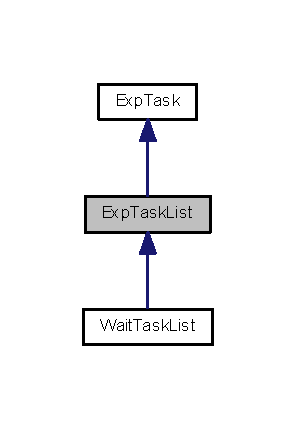
\includegraphics[width=142pt]{class_exp_task_list__inherit__graph}
\end{center}
\end{figure}
\subsection*{Public Slots}
\begin{DoxyCompactItemize}
\item 
virtual void \hyperlink{class_exp_task_list_aac7d8753382c988d39d2a3054ed2c7aa}{start} ()
\begin{DoxyCompactList}\small\item\em This method starts execution of the \hyperlink{class_exp_task}{Exp\+Task} object contained in the \hyperlink{class_exp_task_list}{Exp\+Task\+List}. \end{DoxyCompactList}\item 
virtual void \hyperlink{class_exp_task_list_ae3542825c792c23c1f2a54b9d63074d1}{stop} ()
\begin{DoxyCompactList}\small\item\em This methods stops execution of the \hyperlink{class_exp_task_list}{Exp\+Task\+List} and current running \hyperlink{class_exp_task}{Exp\+Task} through the emitting the \hyperlink{class_exp_task_list_a445b0e774f24ebcd351ef5121d7f9487}{stop\+Task()} signal. \end{DoxyCompactList}\end{DoxyCompactItemize}
\subsection*{Signals}
\begin{DoxyCompactItemize}
\item 
\hypertarget{class_exp_task_list_a445b0e774f24ebcd351ef5121d7f9487}{}void \hyperlink{class_exp_task_list_a445b0e774f24ebcd351ef5121d7f9487}{stop\+Task} ()\label{class_exp_task_list_a445b0e774f24ebcd351ef5121d7f9487}

\begin{DoxyCompactList}\small\item\em This signal is emited form the \hyperlink{class_exp_task_list_ae3542825c792c23c1f2a54b9d63074d1}{stop()} method and is connected in the \hyperlink{class_exp_task_list_a2aa559b46e0fa585386fdf209ab2f366}{next\+Task()} method to the \hyperlink{class_exp_task_a22f581786f11fa3c7dc52ff90c6b7043}{Exp\+Task\+::stop()} slot of the current running \hyperlink{class_exp_task}{Exp\+Task}. \end{DoxyCompactList}\end{DoxyCompactItemize}
\subsection*{Public Member Functions}
\begin{DoxyCompactItemize}
\item 
\hyperlink{class_exp_task_list_a8641c39dd170ede0b12a7f17997db03c}{Exp\+Task\+List} (Q\+Object $\ast$parent=0)
\begin{DoxyCompactList}\small\item\em Creates \hyperlink{class_exp_task_list}{Exp\+Task\+List} object. \end{DoxyCompactList}\item 
\hypertarget{class_exp_task_list_ad65ef5ef9a9826428de3ed56c577c40c}{}virtual \hyperlink{class_exp_task_list_ad65ef5ef9a9826428de3ed56c577c40c}{$\sim$\+Exp\+Task\+List} ()\label{class_exp_task_list_ad65ef5ef9a9826428de3ed56c577c40c}

\begin{DoxyCompactList}\small\item\em Destroyes \hyperlink{class_exp_task_list}{Exp\+Task\+List}, deletes all \hyperlink{struct_exp_task_list_traits_1_1_task_item}{Exp\+Task\+List\+Traits\+::\+Task\+Item} objects from the task list. \end{DoxyCompactList}\item 
virtual void \hyperlink{class_exp_task_list_a3e582c5e9ce6f23f86de96d885277fd2}{add\+Task} (\hyperlink{struct_exp_task_list_traits_1_1_task_item}{Exp\+Task\+List\+Traits\+::\+Task\+Item} tsk)
\begin{DoxyCompactList}\small\item\em Appends task to the task list. \end{DoxyCompactList}\item 
bool \hyperlink{class_exp_task_list_ab48c2f2cdc847964481885c15d56b8fd}{running} () const 
\begin{DoxyCompactList}\small\item\em This method returns true if the \hyperlink{class_exp_task_list}{Exp\+Task\+List} is executing its content. \end{DoxyCompactList}\item 
bool \hyperlink{class_exp_task_list_a791b0db466c6144af5fbe9e9954aaa9a}{stop\+Status} () const 
\begin{DoxyCompactList}\small\item\em This method returns true if the \hyperlink{class_exp_task_list}{Exp\+Task\+List} is stopped by the \hyperlink{class_exp_task_list_ae3542825c792c23c1f2a54b9d63074d1}{stop()} method. \end{DoxyCompactList}\item 
bool \hyperlink{class_exp_task_list_afe0b0c53938d3ee5dcd154306bba39e8}{is\+Empty} () const 
\begin{DoxyCompactList}\small\item\em This method returns true if \hyperlink{class_exp_task_list}{Exp\+Task\+List} does not contain any \hyperlink{struct_exp_task_list_traits_1_1_task_item}{Exp\+Task\+List\+Traits\+::\+Task\+Item}. \end{DoxyCompactList}\item 
\hyperlink{struct_exp_task_list_traits_1_1_task_item}{Exp\+Task\+List\+Traits\+::\+Task\+Item} \hyperlink{class_exp_task_list_a9a99c3b7f558ec7248019d1323e22256}{get\+Curr\+Task} () const 
\begin{DoxyCompactList}\small\item\em This method returns the current running task. \end{DoxyCompactList}\item 
const Q\+List$<$ \hyperlink{struct_exp_task_list_traits_1_1_task_item}{Exp\+Task\+List\+Traits\+::\+Task\+Item} $>$ \& \hyperlink{class_exp_task_list_a608f181f27787a3e72c2388cc47ca177}{get\+Tasks} () const 
\begin{DoxyCompactList}\small\item\em This method returns the reference to the list containing all stored tasks. \end{DoxyCompactList}\end{DoxyCompactItemize}
\subsection*{Protected Slots}
\begin{DoxyCompactItemize}
\item 
virtual void \hyperlink{class_exp_task_list_afba27c0ec9da9a87cea6a15fc5a2beca}{task\+Finished} ()
\begin{DoxyCompactList}\small\item\em This method is connected to the \hyperlink{class_exp_task_aeb51d072a7b96f55da3738a8c7733611}{Exp\+Task\+::finished()} signal of the current task and handles repeating of its execution until the intended number of executions is reached. \end{DoxyCompactList}\end{DoxyCompactItemize}
\subsection*{Protected Member Functions}
\begin{DoxyCompactItemize}
\item 
virtual void \hyperlink{class_exp_task_list_adee3f2e0894b5b102b2fcf0cff4ff25a}{task\+List\+Finished} ()
\begin{DoxyCompactList}\small\item\em This method is executed after the \hyperlink{class_exp_task_list}{Exp\+Task\+List} finishes execution of all contained \hyperlink{class_exp_task}{Exp\+Task} objects. \end{DoxyCompactList}\item 
\hypertarget{class_exp_task_list_a2aa559b46e0fa585386fdf209ab2f366}{}virtual void \hyperlink{class_exp_task_list_a2aa559b46e0fa585386fdf209ab2f366}{next\+Task} ()\label{class_exp_task_list_a2aa559b46e0fa585386fdf209ab2f366}

\begin{DoxyCompactList}\small\item\em Executes a next \hyperlink{class_exp_task}{Exp\+Task}. The \hyperlink{struct_exp_task_list_traits_1_1_task_item}{Exp\+Task\+List\+Traits\+::\+Task\+Item} objects which contain \hyperlink{class_exp_task}{Exp\+Task} objects are saved in \hyperlink{class_exp_task_list_abfeadd157333249e79ee8ff98ba98cf2}{Exp\+Task\+List\+::curr\+Tasks}, where first element is that, which will by next executed. If there is no task in list, \hyperlink{class_exp_task_list_adee3f2e0894b5b102b2fcf0cff4ff25a}{task\+List\+Finished()} method is called. The \hyperlink{class_exp_task}{Exp\+Task}\textquotesingle{}s \hyperlink{class_exp_task_aeb51d072a7b96f55da3738a8c7733611}{Exp\+Task\+::finished()} signal is connected to the \hyperlink{class_exp_task_list_afba27c0ec9da9a87cea6a15fc5a2beca}{task\+Finished()} slot and \hyperlink{class_exp_task_list_a445b0e774f24ebcd351ef5121d7f9487}{stop\+Task()} signal is connected to the \hyperlink{class_exp_task}{Exp\+Task}\textquotesingle{}s \hyperlink{class_exp_task_a22f581786f11fa3c7dc52ff90c6b7043}{Exp\+Task\+::stop()} slot. If the current \hyperlink{class_exp_task}{Exp\+Task} has not \hyperlink{class_exp_task_a1ab988b6d9eb6d61cd1b3ac1a1c42153}{Exp\+Task\+::curr\+Times\+Exec()} greater than zero, the \hyperlink{class_exp_task_list_afba27c0ec9da9a87cea6a15fc5a2beca}{task\+Finished()} method is called. \end{DoxyCompactList}\end{DoxyCompactItemize}
\subsection*{Private Attributes}
\begin{DoxyCompactItemize}
\item 
\hypertarget{class_exp_task_list_a2c6fef3959dbd632a927ca789f657d05}{}Q\+List$<$ \hyperlink{struct_exp_task_list_traits_1_1_task_item}{Exp\+Task\+List\+Traits\+::\+Task\+Item} $>$ \hyperlink{class_exp_task_list_a2c6fef3959dbd632a927ca789f657d05}{tasks}\label{class_exp_task_list_a2c6fef3959dbd632a927ca789f657d05}

\begin{DoxyCompactList}\small\item\em Private variable containing all tasks to be executed. \end{DoxyCompactList}\item 
\hypertarget{class_exp_task_list_abfeadd157333249e79ee8ff98ba98cf2}{}Q\+List$<$ \hyperlink{struct_exp_task_list_traits_1_1_task_item}{Exp\+Task\+List\+Traits\+::\+Task\+Item} $>$ \hyperlink{class_exp_task_list_abfeadd157333249e79ee8ff98ba98cf2}{curr\+Tasks}\label{class_exp_task_list_abfeadd157333249e79ee8ff98ba98cf2}

\begin{DoxyCompactList}\small\item\em Private varibale containing current task list. It do not store tasks which were already executed in current run even though they will be executed in next run of the list. \end{DoxyCompactList}\item 
\hypertarget{class_exp_task_list_a1f3833f849f349d37a44a69b09b547b6}{}bool \hyperlink{class_exp_task_list_a1f3833f849f349d37a44a69b09b547b6}{bl\+Running}\label{class_exp_task_list_a1f3833f849f349d37a44a69b09b547b6}

\begin{DoxyCompactList}\small\item\em true if \hyperlink{class_exp_task_list}{Exp\+Task\+List} is running \end{DoxyCompactList}\item 
\hypertarget{class_exp_task_list_aa7bfbd7aece2b214647e15d26b32905b}{}bool \hyperlink{class_exp_task_list_aa7bfbd7aece2b214647e15d26b32905b}{bl\+Stop}\label{class_exp_task_list_aa7bfbd7aece2b214647e15d26b32905b}

\begin{DoxyCompactList}\small\item\em true if \hyperlink{class_exp_task_list_ae3542825c792c23c1f2a54b9d63074d1}{stop()} method is stopping or has stopped the \hyperlink{class_exp_task_list}{Exp\+Task\+List} execution. \end{DoxyCompactList}\end{DoxyCompactItemize}


\subsection{Detailed Description}
\hyperlink{class_exp_task_list}{Exp\+Task\+List}. 

\subsection{Constructor \& Destructor Documentation}
\hypertarget{class_exp_task_list_a8641c39dd170ede0b12a7f17997db03c}{}\index{Exp\+Task\+List@{Exp\+Task\+List}!Exp\+Task\+List@{Exp\+Task\+List}}
\index{Exp\+Task\+List@{Exp\+Task\+List}!Exp\+Task\+List@{Exp\+Task\+List}}
\subsubsection[{Exp\+Task\+List}]{\setlength{\rightskip}{0pt plus 5cm}Exp\+Task\+List\+::\+Exp\+Task\+List (
\begin{DoxyParamCaption}
\item[{Q\+Object $\ast$}]{parent = {\ttfamily 0}}
\end{DoxyParamCaption}
)\hspace{0.3cm}{\ttfamily [explicit]}}\label{class_exp_task_list_a8641c39dd170ede0b12a7f17997db03c}


Creates \hyperlink{class_exp_task_list}{Exp\+Task\+List} object. 


\begin{DoxyParams}{Parameters}
{\em parent} & A parent Q\+Objet in Qt\textquotesingle{}s ownership system. \\
\hline
\end{DoxyParams}


\subsection{Member Function Documentation}
\hypertarget{class_exp_task_list_a3e582c5e9ce6f23f86de96d885277fd2}{}\index{Exp\+Task\+List@{Exp\+Task\+List}!add\+Task@{add\+Task}}
\index{add\+Task@{add\+Task}!Exp\+Task\+List@{Exp\+Task\+List}}
\subsubsection[{add\+Task}]{\setlength{\rightskip}{0pt plus 5cm}void Exp\+Task\+List\+::add\+Task (
\begin{DoxyParamCaption}
\item[{{\bf Exp\+Task\+List\+Traits\+::\+Task\+Item}}]{tsk}
\end{DoxyParamCaption}
)\hspace{0.3cm}{\ttfamily [virtual]}}\label{class_exp_task_list_a3e582c5e9ce6f23f86de96d885277fd2}


Appends task to the task list. 


\begin{DoxyParams}{Parameters}
{\em tsk} & appended task. \\
\hline
\end{DoxyParams}


Reimplemented in \hyperlink{class_wait_task_list_a429d0b45f82a2eef00c5dacffbbc1f70}{Wait\+Task\+List}.

\hypertarget{class_exp_task_list_ab48c2f2cdc847964481885c15d56b8fd}{}\index{Exp\+Task\+List@{Exp\+Task\+List}!running@{running}}
\index{running@{running}!Exp\+Task\+List@{Exp\+Task\+List}}
\subsubsection[{running}]{\setlength{\rightskip}{0pt plus 5cm}Exp\+Task\+List\+::running (
\begin{DoxyParamCaption}
{}
\end{DoxyParamCaption}
) const\hspace{0.3cm}{\ttfamily [inline]}}\label{class_exp_task_list_ab48c2f2cdc847964481885c15d56b8fd}


This method returns true if the \hyperlink{class_exp_task_list}{Exp\+Task\+List} is executing its content. 

\begin{DoxyReturn}{Returns}
true if \hyperlink{class_exp_task_list}{Exp\+Task\+List} is running.
\end{DoxyReturn}
\begin{DoxySeeAlso}{See also}
\hyperlink{class_exp_task_list_aac7d8753382c988d39d2a3054ed2c7aa}{start()}, \hyperlink{class_exp_task_list_ae3542825c792c23c1f2a54b9d63074d1}{stop()} 
\end{DoxySeeAlso}
\hypertarget{class_exp_task_list_a791b0db466c6144af5fbe9e9954aaa9a}{}\index{Exp\+Task\+List@{Exp\+Task\+List}!stop\+Status@{stop\+Status}}
\index{stop\+Status@{stop\+Status}!Exp\+Task\+List@{Exp\+Task\+List}}
\subsubsection[{stop\+Status}]{\setlength{\rightskip}{0pt plus 5cm}bool Exp\+Task\+List\+::stop\+Status (
\begin{DoxyParamCaption}
{}
\end{DoxyParamCaption}
) const}\label{class_exp_task_list_a791b0db466c6144af5fbe9e9954aaa9a}


This method returns true if the \hyperlink{class_exp_task_list}{Exp\+Task\+List} is stopped by the \hyperlink{class_exp_task_list_ae3542825c792c23c1f2a54b9d63074d1}{stop()} method. 

\begin{DoxyReturn}{Returns}
true if \hyperlink{class_exp_task_list}{Exp\+Task\+List} is stopped. 
\end{DoxyReturn}
\hypertarget{class_exp_task_list_afe0b0c53938d3ee5dcd154306bba39e8}{}\index{Exp\+Task\+List@{Exp\+Task\+List}!is\+Empty@{is\+Empty}}
\index{is\+Empty@{is\+Empty}!Exp\+Task\+List@{Exp\+Task\+List}}
\subsubsection[{is\+Empty}]{\setlength{\rightskip}{0pt plus 5cm}bool Exp\+Task\+List\+::is\+Empty (
\begin{DoxyParamCaption}
{}
\end{DoxyParamCaption}
) const}\label{class_exp_task_list_afe0b0c53938d3ee5dcd154306bba39e8}


This method returns true if \hyperlink{class_exp_task_list}{Exp\+Task\+List} does not contain any \hyperlink{struct_exp_task_list_traits_1_1_task_item}{Exp\+Task\+List\+Traits\+::\+Task\+Item}. 

\begin{DoxyReturn}{Returns}
true if \hyperlink{class_exp_task_list}{Exp\+Task\+List} is empty. 
\end{DoxyReturn}
\hypertarget{class_exp_task_list_a9a99c3b7f558ec7248019d1323e22256}{}\index{Exp\+Task\+List@{Exp\+Task\+List}!get\+Curr\+Task@{get\+Curr\+Task}}
\index{get\+Curr\+Task@{get\+Curr\+Task}!Exp\+Task\+List@{Exp\+Task\+List}}
\subsubsection[{get\+Curr\+Task}]{\setlength{\rightskip}{0pt plus 5cm}{\bf Exp\+Task\+List\+Traits\+::\+Task\+Item} Exp\+Task\+List\+::get\+Curr\+Task (
\begin{DoxyParamCaption}
{}
\end{DoxyParamCaption}
) const}\label{class_exp_task_list_a9a99c3b7f558ec7248019d1323e22256}


This method returns the current running task. 

\begin{DoxyReturn}{Returns}
current running task 
\end{DoxyReturn}
\hypertarget{class_exp_task_list_a608f181f27787a3e72c2388cc47ca177}{}\index{Exp\+Task\+List@{Exp\+Task\+List}!get\+Tasks@{get\+Tasks}}
\index{get\+Tasks@{get\+Tasks}!Exp\+Task\+List@{Exp\+Task\+List}}
\subsubsection[{get\+Tasks}]{\setlength{\rightskip}{0pt plus 5cm}Exp\+Task\+List\+::get\+Tasks (
\begin{DoxyParamCaption}
{}
\end{DoxyParamCaption}
) const\hspace{0.3cm}{\ttfamily [inline]}}\label{class_exp_task_list_a608f181f27787a3e72c2388cc47ca177}


This method returns the reference to the list containing all stored tasks. 

\begin{DoxyReturn}{Returns}
list containing all stored tasks. 
\end{DoxyReturn}
\hypertarget{class_exp_task_list_aac7d8753382c988d39d2a3054ed2c7aa}{}\index{Exp\+Task\+List@{Exp\+Task\+List}!start@{start}}
\index{start@{start}!Exp\+Task\+List@{Exp\+Task\+List}}
\subsubsection[{start}]{\setlength{\rightskip}{0pt plus 5cm}void Exp\+Task\+List\+::start (
\begin{DoxyParamCaption}
{}
\end{DoxyParamCaption}
)\hspace{0.3cm}{\ttfamily [virtual]}, {\ttfamily [slot]}}\label{class_exp_task_list_aac7d8753382c988d39d2a3054ed2c7aa}


This method starts execution of the \hyperlink{class_exp_task}{Exp\+Task} object contained in the \hyperlink{class_exp_task_list}{Exp\+Task\+List}. 

At first, this method controlls if the \hyperlink{class_exp_task_list}{Exp\+Task\+List} is not already running. If yes, it skips the request, it the other case, it sets private variables indicating \hyperlink{class_exp_task_list}{Exp\+Task\+List} state and calls nex\+Task() method.

\begin{DoxySeeAlso}{See also}
\hyperlink{class_exp_task_list_ae3542825c792c23c1f2a54b9d63074d1}{stop()}, \hyperlink{class_exp_task_list_afba27c0ec9da9a87cea6a15fc5a2beca}{task\+Finished()}, \hyperlink{class_exp_task_list_adee3f2e0894b5b102b2fcf0cff4ff25a}{task\+List\+Finished()} 
\end{DoxySeeAlso}
\hypertarget{class_exp_task_list_ae3542825c792c23c1f2a54b9d63074d1}{}\index{Exp\+Task\+List@{Exp\+Task\+List}!stop@{stop}}
\index{stop@{stop}!Exp\+Task\+List@{Exp\+Task\+List}}
\subsubsection[{stop}]{\setlength{\rightskip}{0pt plus 5cm}void Exp\+Task\+List\+::stop (
\begin{DoxyParamCaption}
{}
\end{DoxyParamCaption}
)\hspace{0.3cm}{\ttfamily [virtual]}, {\ttfamily [slot]}}\label{class_exp_task_list_ae3542825c792c23c1f2a54b9d63074d1}


This methods stops execution of the \hyperlink{class_exp_task_list}{Exp\+Task\+List} and current running \hyperlink{class_exp_task}{Exp\+Task} through the emitting the \hyperlink{class_exp_task_list_a445b0e774f24ebcd351ef5121d7f9487}{stop\+Task()} signal. 

After the current running \hyperlink{class_exp_task}{Exp\+Task} is finished, all the contained \hyperlink{class_exp_task}{Exp\+Task} objects are deleted and all the \hyperlink{struct_exp_task_list_traits_1_1_task_item}{Exp\+Task\+List\+Traits\+::\+Task\+Item} structs are removed from the list and the \hyperlink{class_exp_task_list_adee3f2e0894b5b102b2fcf0cff4ff25a}{task\+List\+Finished()} method is called, which emits \hyperlink{class_exp_task_a1a766503f6eb22b82c6e31e279b0ea9d}{task\+Failed()} and \hyperlink{class_exp_task_aeb51d072a7b96f55da3738a8c7733611}{finished()} signals. \hypertarget{class_exp_task_list_adee3f2e0894b5b102b2fcf0cff4ff25a}{}\index{Exp\+Task\+List@{Exp\+Task\+List}!task\+List\+Finished@{task\+List\+Finished}}
\index{task\+List\+Finished@{task\+List\+Finished}!Exp\+Task\+List@{Exp\+Task\+List}}
\subsubsection[{task\+List\+Finished}]{\setlength{\rightskip}{0pt plus 5cm}void Exp\+Task\+List\+::task\+List\+Finished (
\begin{DoxyParamCaption}
{}
\end{DoxyParamCaption}
)\hspace{0.3cm}{\ttfamily [protected]}, {\ttfamily [virtual]}}\label{class_exp_task_list_adee3f2e0894b5b102b2fcf0cff4ff25a}


This method is executed after the \hyperlink{class_exp_task_list}{Exp\+Task\+List} finishes execution of all contained \hyperlink{class_exp_task}{Exp\+Task} objects. 

It emits \hyperlink{class_exp_task_a1a766503f6eb22b82c6e31e279b0ea9d}{task\+Failed()} signal if this is a consequence of \hyperlink{class_exp_task_list_ae3542825c792c23c1f2a54b9d63074d1}{stop()} method, while \hyperlink{class_exp_task_list_ab48c2f2cdc847964481885c15d56b8fd}{running()} status is still true. Then it emits \hyperlink{class_exp_task_aeb51d072a7b96f55da3738a8c7733611}{finished()} signal, where the \hyperlink{class_exp_task_list_ab48c2f2cdc847964481885c15d56b8fd}{running()} status is already false. 

Reimplemented in \hyperlink{class_wait_task_list_aa0749dc369379ff737fdf14a89142bd2}{Wait\+Task\+List}.

\hypertarget{class_exp_task_list_afba27c0ec9da9a87cea6a15fc5a2beca}{}\index{Exp\+Task\+List@{Exp\+Task\+List}!task\+Finished@{task\+Finished}}
\index{task\+Finished@{task\+Finished}!Exp\+Task\+List@{Exp\+Task\+List}}
\subsubsection[{task\+Finished}]{\setlength{\rightskip}{0pt plus 5cm}void Exp\+Task\+List\+::task\+Finished (
\begin{DoxyParamCaption}
{}
\end{DoxyParamCaption}
)\hspace{0.3cm}{\ttfamily [protected]}, {\ttfamily [virtual]}, {\ttfamily [slot]}}\label{class_exp_task_list_afba27c0ec9da9a87cea6a15fc5a2beca}


This method is connected to the \hyperlink{class_exp_task_aeb51d072a7b96f55da3738a8c7733611}{Exp\+Task\+::finished()} signal of the current task and handles repeating of its execution until the intended number of executions is reached. 

At first, the method controlls if the task was stopped by the stop method and if so, it cleans up containing tasks and executes \hyperlink{class_exp_task_list_adee3f2e0894b5b102b2fcf0cff4ff25a}{task\+List\+Finished()}.

Then it decreases \hyperlink{class_exp_task}{Exp\+Task}\textquotesingle{}s execution counter by the \hyperlink{class_exp_task_a4b1e37a956ea18764bb62b8b9ffa52d3}{Exp\+Task\+::once\+Executed()} method and executes it once more if the counter is styl greater than one, else it disconnects the the \hyperlink{class_exp_task_aeb51d072a7b96f55da3738a8c7733611}{Exp\+Task\+::finished()} signal from this method and \hyperlink{class_exp_task_list_a445b0e774f24ebcd351ef5121d7f9487}{Exp\+Task\+List\+::stop\+Task()} signla from \hyperlink{class_exp_task_a22f581786f11fa3c7dc52ff90c6b7043}{Exp\+Task\+::stop()} method. If the task need to be deleted later, it calls \hyperlink{class_exp_task_ac84290f4ee014237657794522350cfea}{Exp\+Task\+::restart\+Times\+Exec()}, else it deletes task and removes it from tasks list. Then it calls \hyperlink{class_exp_task_list_a2aa559b46e0fa585386fdf209ab2f366}{next\+Task()}. 

The documentation for this class was generated from the following files\+:\begin{DoxyCompactItemize}
\item 
exptasklist.\+h\item 
exptasklist.\+cpp\end{DoxyCompactItemize}

\hypertarget{class_fork_join_task}{}\section{Fork\+Join\+Task Class Reference}
\label{class_fork_join_task}\index{Fork\+Join\+Task@{Fork\+Join\+Task}}


This class creates inside multiple \hyperlink{class_exp_task_list}{Exp\+Task\+List} objects and runs each of them in parallel when started, waiting for them all to finish.  




Inheritance diagram for Fork\+Join\+Task\+:\nopagebreak
\begin{figure}[H]
\begin{center}
\leavevmode
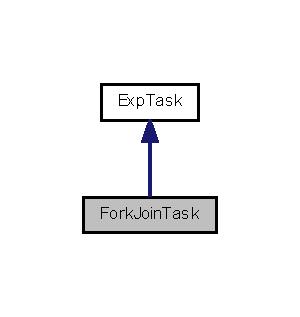
\includegraphics[width=144pt]{class_fork_join_task__inherit__graph}
\end{center}
\end{figure}
\subsection*{Public Slots}
\begin{DoxyCompactItemize}
\item 
\hypertarget{class_fork_join_task_a9a812b83e31dc58c6850d36b16008f0e}{}virtual void \hyperlink{class_fork_join_task_a9a812b83e31dc58c6850d36b16008f0e}{start} ()\label{class_fork_join_task_a9a812b83e31dc58c6850d36b16008f0e}

\begin{DoxyCompactList}\small\item\em Starts all contained threads (\hyperlink{class_exp_task_list}{Exp\+Task\+List} objects). \end{DoxyCompactList}\item 
\hypertarget{class_fork_join_task_adbd84bb9658e533fa4ca21841daedcc5}{}virtual void \hyperlink{class_fork_join_task_adbd84bb9658e533fa4ca21841daedcc5}{stop} ()\label{class_fork_join_task_adbd84bb9658e533fa4ca21841daedcc5}

\begin{DoxyCompactList}\small\item\em Stops all contained threads (\hyperlink{class_exp_task_list}{Exp\+Task\+List} objects). \end{DoxyCompactList}\end{DoxyCompactItemize}
\subsection*{Public Member Functions}
\begin{DoxyCompactItemize}
\item 
\hyperlink{class_fork_join_task_a2be71d32906e00a7776655768419a3a3}{Fork\+Join\+Task} (unsigned int threads\+N=2, Q\+Object $\ast$parent=0)
\begin{DoxyCompactList}\small\item\em Constructs \hyperlink{class_fork_join_task}{Fork\+Join\+Task} object. \end{DoxyCompactList}\item 
\hypertarget{class_fork_join_task_ac6ff10aa0b6d5cead09b630adabe8cef}{}virtual \hyperlink{class_fork_join_task_ac6ff10aa0b6d5cead09b630adabe8cef}{$\sim$\+Fork\+Join\+Task} ()\label{class_fork_join_task_ac6ff10aa0b6d5cead09b630adabe8cef}

\begin{DoxyCompactList}\small\item\em Destroyes \hyperlink{class_fork_join_task}{Fork\+Join\+Task} object. \end{DoxyCompactList}\item 
void \hyperlink{class_fork_join_task_aff58c038df10cd36fa8842486fa46d09}{add\+Task} (\hyperlink{struct_exp_task_list_traits_1_1_task_item}{Exp\+Task\+List\+Traits\+::\+Task\+Item} tsk, unsigned int threadno)
\begin{DoxyCompactList}\small\item\em Adds task to the particular thread by the \hyperlink{class_exp_task_list_a3e582c5e9ce6f23f86de96d885277fd2}{Exp\+Task\+List\+::add\+Task()} method. \end{DoxyCompactList}\item 
\hypertarget{class_fork_join_task_aaad36fef1a41e7ec3056e2d70d79c628}{}unsigned int \hyperlink{class_fork_join_task_aaad36fef1a41e7ec3056e2d70d79c628}{get\+Threads\+N} () const \label{class_fork_join_task_aaad36fef1a41e7ec3056e2d70d79c628}

\begin{DoxyCompactList}\small\item\em Gets number of threads. \end{DoxyCompactList}\end{DoxyCompactItemize}
\subsection*{Protected Member Functions}
\begin{DoxyCompactItemize}
\item 
\hypertarget{class_fork_join_task_a8bb596c1e3ffc59e2302c2d19273da76}{}const Q\+List$<$ \hyperlink{struct_exp_task_list_traits_1_1_task_item}{Exp\+Task\+List\+Traits\+::\+Task\+Item} $>$ \& \hyperlink{class_fork_join_task_a8bb596c1e3ffc59e2302c2d19273da76}{get\+Tasks} (unsigned int threadno) const \label{class_fork_join_task_a8bb596c1e3ffc59e2302c2d19273da76}

\begin{DoxyCompactList}\small\item\em Gets all tasks from the particular thread (\hyperlink{class_exp_task_list}{Exp\+Task\+List} objects). \end{DoxyCompactList}\end{DoxyCompactItemize}
\subsection*{Private Attributes}
\begin{DoxyCompactItemize}
\item 
\hypertarget{class_fork_join_task_a3225694976a00691c7468d4c5126cf74}{}Q\+Vector$<$ \hyperlink{class_exp_task_list}{Exp\+Task\+List} $\ast$ $>$ \hyperlink{class_fork_join_task_a3225694976a00691c7468d4c5126cf74}{exp\+Task\+Lists}\label{class_fork_join_task_a3225694976a00691c7468d4c5126cf74}

\begin{DoxyCompactList}\small\item\em contained threads (\hyperlink{class_exp_task_list}{Exp\+Task\+List} objects). \end{DoxyCompactList}\item 
\hypertarget{class_fork_join_task_ac5051eb583219076a4b6e4157490abf7}{}unsigned int \hyperlink{class_fork_join_task_ac5051eb583219076a4b6e4157490abf7}{threads\+N\+\_\+}\label{class_fork_join_task_ac5051eb583219076a4b6e4157490abf7}

\begin{DoxyCompactList}\small\item\em number of contained threads (\hyperlink{class_exp_task_list}{Exp\+Task\+List} objects). \end{DoxyCompactList}\end{DoxyCompactItemize}
\subsection*{Friends}
\begin{DoxyCompactItemize}
\item 
\hypertarget{class_fork_join_task_a147f773ea07af65ac2105d1ac1208693}{}class {\bfseries Wait\+Task\+List}\label{class_fork_join_task_a147f773ea07af65ac2105d1ac1208693}

\end{DoxyCompactItemize}
\subsection*{Additional Inherited Members}


\subsection{Detailed Description}
This class creates inside multiple \hyperlink{class_exp_task_list}{Exp\+Task\+List} objects and runs each of them in parallel when started, waiting for them all to finish. 

\subsection{Constructor \& Destructor Documentation}
\hypertarget{class_fork_join_task_a2be71d32906e00a7776655768419a3a3}{}\index{Fork\+Join\+Task@{Fork\+Join\+Task}!Fork\+Join\+Task@{Fork\+Join\+Task}}
\index{Fork\+Join\+Task@{Fork\+Join\+Task}!Fork\+Join\+Task@{Fork\+Join\+Task}}
\subsubsection[{Fork\+Join\+Task}]{\setlength{\rightskip}{0pt plus 5cm}Fork\+Join\+Task\+::\+Fork\+Join\+Task (
\begin{DoxyParamCaption}
\item[{unsigned int}]{threads\+N = {\ttfamily 2}, }
\item[{Q\+Object $\ast$}]{parent = {\ttfamily 0}}
\end{DoxyParamCaption}
)\hspace{0.3cm}{\ttfamily [explicit]}}\label{class_fork_join_task_a2be71d32906e00a7776655768419a3a3}


Constructs \hyperlink{class_fork_join_task}{Fork\+Join\+Task} object. 


\begin{DoxyParams}{Parameters}
{\em threads\+N} & The number of required threads \\
\hline
{\em parent} & A parent in Qt\textquotesingle{}s ownership system. \\
\hline
\end{DoxyParams}


\subsection{Member Function Documentation}
\hypertarget{class_fork_join_task_aff58c038df10cd36fa8842486fa46d09}{}\index{Fork\+Join\+Task@{Fork\+Join\+Task}!add\+Task@{add\+Task}}
\index{add\+Task@{add\+Task}!Fork\+Join\+Task@{Fork\+Join\+Task}}
\subsubsection[{add\+Task}]{\setlength{\rightskip}{0pt plus 5cm}void Fork\+Join\+Task\+::add\+Task (
\begin{DoxyParamCaption}
\item[{{\bf Exp\+Task\+List\+Traits\+::\+Task\+Item}}]{tsk, }
\item[{unsigned int}]{threadno}
\end{DoxyParamCaption}
)}\label{class_fork_join_task_aff58c038df10cd36fa8842486fa46d09}


Adds task to the particular thread by the \hyperlink{class_exp_task_list_a3e582c5e9ce6f23f86de96d885277fd2}{Exp\+Task\+List\+::add\+Task()} method. 


\begin{DoxyParams}{Parameters}
{\em tsk} & added task \\
\hline
{\em threadno} & thread number \\
\hline
\end{DoxyParams}


The documentation for this class was generated from the following files\+:\begin{DoxyCompactItemize}
\item 
exptasklist.\+h\item 
exptasklist.\+cpp\end{DoxyCompactItemize}

\hypertarget{struct_wait_task_list_traits_1_1_task_item}{}\section{Wait\+Task\+List\+Traits\+:\+:Task\+Item Struct Reference}
\label{struct_wait_task_list_traits_1_1_task_item}\index{Wait\+Task\+List\+Traits\+::\+Task\+Item@{Wait\+Task\+List\+Traits\+::\+Task\+Item}}


Container for \hyperlink{class_wait_task}{Wait\+Task} attaching to it its type for faster runtime identification.  


\subsection*{Public Member Functions}
\begin{DoxyCompactItemize}
\item 
\hyperlink{struct_wait_task_list_traits_1_1_task_item_a6bf127a8e7b4c7a05e2957035e252366}{Task\+Item} (\hyperlink{namespace_wait_task_list_traits_a3cb74ee1929f03e51486087ef21caf9f}{Wait\+For} wf=\hyperlink{namespace_wait_task_list_traits_a3cb74ee1929f03e51486087ef21caf9fa6adf97f83acf6453d4a6a4b1070f3754}{Wait\+For\+::\+None}, \hyperlink{class_wait_task}{Wait\+Task} $\ast$wt=nullptr)
\begin{DoxyCompactList}\small\item\em Constructs the \hyperlink{struct_wait_task_list_traits_1_1_task_item}{Task\+Item} stuct. \end{DoxyCompactList}\end{DoxyCompactItemize}
\subsection*{Data Fields}
\begin{DoxyCompactItemize}
\item 
\hypertarget{struct_wait_task_list_traits_1_1_task_item_a1e715ba11a4776b3d798538fe75bacd6}{}\hyperlink{class_wait_task}{Wait\+Task} $\ast$ \hyperlink{struct_wait_task_list_traits_1_1_task_item_a1e715ba11a4776b3d798538fe75bacd6}{task}\label{struct_wait_task_list_traits_1_1_task_item_a1e715ba11a4776b3d798538fe75bacd6}

\begin{DoxyCompactList}\small\item\em the \hyperlink{class_wait_task}{Wait\+Task} \end{DoxyCompactList}\item 
\hypertarget{struct_wait_task_list_traits_1_1_task_item_a102b0dbbd5d466f5a05091d914fa8d61}{}\hyperlink{namespace_wait_task_list_traits_a3cb74ee1929f03e51486087ef21caf9f}{Wait\+For} \hyperlink{struct_wait_task_list_traits_1_1_task_item_a102b0dbbd5d466f5a05091d914fa8d61}{wait\+For}\label{struct_wait_task_list_traits_1_1_task_item_a102b0dbbd5d466f5a05091d914fa8d61}

\begin{DoxyCompactList}\small\item\em the Wait\+For \end{DoxyCompactList}\end{DoxyCompactItemize}


\subsection{Detailed Description}
Container for \hyperlink{class_wait_task}{Wait\+Task} attaching to it its type for faster runtime identification. 

\begin{DoxySeeAlso}{See also}
Task\+Type 
\end{DoxySeeAlso}


\subsection{Constructor \& Destructor Documentation}
\hypertarget{struct_wait_task_list_traits_1_1_task_item_a6bf127a8e7b4c7a05e2957035e252366}{}\index{Wait\+Task\+List\+Traits\+::\+Task\+Item@{Wait\+Task\+List\+Traits\+::\+Task\+Item}!Task\+Item@{Task\+Item}}
\index{Task\+Item@{Task\+Item}!Wait\+Task\+List\+Traits\+::\+Task\+Item@{Wait\+Task\+List\+Traits\+::\+Task\+Item}}
\subsubsection[{Task\+Item}]{\setlength{\rightskip}{0pt plus 5cm}Wait\+Task\+List\+Traits\+::\+Task\+Item\+::\+Task\+Item (
\begin{DoxyParamCaption}
\item[{{\bf Wait\+For}}]{wf = {\ttfamily {\bf Wait\+For\+::\+None}}, }
\item[{{\bf Wait\+Task} $\ast$}]{wt = {\ttfamily nullptr}}
\end{DoxyParamCaption}
)\hspace{0.3cm}{\ttfamily [inline]}}\label{struct_wait_task_list_traits_1_1_task_item_a6bf127a8e7b4c7a05e2957035e252366}


Constructs the \hyperlink{struct_wait_task_list_traits_1_1_task_item}{Task\+Item} stuct. 


\begin{DoxyParams}{Parameters}
{\em wf} & type of the task \\
\hline
{\em wt} & a pointer to the task \\
\hline
\end{DoxyParams}


The documentation for this struct was generated from the following files\+:\begin{DoxyCompactItemize}
\item 
waittasklist.\+h\item 
waittasklist.\+cpp\end{DoxyCompactItemize}

\hypertarget{struct_exp_task_list_traits_1_1_task_item}{}\section{Exp\+Task\+List\+Traits\+:\+:Task\+Item Struct Reference}
\label{struct_exp_task_list_traits_1_1_task_item}\index{Exp\+Task\+List\+Traits\+::\+Task\+Item@{Exp\+Task\+List\+Traits\+::\+Task\+Item}}


Container for \hyperlink{class_exp_task}{Exp\+Task} attaching to it its type for faster runtime identification.  


\subsection*{Public Member Functions}
\begin{DoxyCompactItemize}
\item 
\hyperlink{struct_exp_task_list_traits_1_1_task_item_ab8d50b8bac433cef79b948b1341b09e2}{Task\+Item} (\hyperlink{namespace_exp_task_list_traits_adcf9a5159b43c6df6f5e6835170c25b2}{Task\+Type} tt=\hyperlink{namespace_exp_task_list_traits_adcf9a5159b43c6df6f5e6835170c25b2a6adf97f83acf6453d4a6a4b1070f3754}{Task\+Type\+::\+None}, \hyperlink{class_exp_task}{Exp\+Task} $\ast$t=nullptr)
\begin{DoxyCompactList}\small\item\em Constructs the \hyperlink{struct_exp_task_list_traits_1_1_task_item}{Task\+Item} stuct. \end{DoxyCompactList}\end{DoxyCompactItemize}
\subsection*{Data Fields}
\begin{DoxyCompactItemize}
\item 
\hypertarget{struct_exp_task_list_traits_1_1_task_item_ab286c3da7c53f72bff6c045d1796d5f7}{}\hyperlink{class_exp_task}{Exp\+Task} $\ast$ \hyperlink{struct_exp_task_list_traits_1_1_task_item_ab286c3da7c53f72bff6c045d1796d5f7}{task}\label{struct_exp_task_list_traits_1_1_task_item_ab286c3da7c53f72bff6c045d1796d5f7}

\begin{DoxyCompactList}\small\item\em the \hyperlink{class_exp_task}{Exp\+Task} \end{DoxyCompactList}\item 
\hypertarget{struct_exp_task_list_traits_1_1_task_item_a0531e3bff4d273fbf76cd4b65838c78a}{}\hyperlink{namespace_exp_task_list_traits_adcf9a5159b43c6df6f5e6835170c25b2}{Task\+Type} \hyperlink{struct_exp_task_list_traits_1_1_task_item_a0531e3bff4d273fbf76cd4b65838c78a}{task\+Type}\label{struct_exp_task_list_traits_1_1_task_item_a0531e3bff4d273fbf76cd4b65838c78a}

\begin{DoxyCompactList}\small\item\em the Task\+Type \end{DoxyCompactList}\end{DoxyCompactItemize}


\subsection{Detailed Description}
Container for \hyperlink{class_exp_task}{Exp\+Task} attaching to it its type for faster runtime identification. 

\begin{DoxySeeAlso}{See also}
\hyperlink{namespace_exp_task_list_traits_adcf9a5159b43c6df6f5e6835170c25b2}{Task\+Type} 
\end{DoxySeeAlso}


\subsection{Constructor \& Destructor Documentation}
\hypertarget{struct_exp_task_list_traits_1_1_task_item_ab8d50b8bac433cef79b948b1341b09e2}{}\index{Exp\+Task\+List\+Traits\+::\+Task\+Item@{Exp\+Task\+List\+Traits\+::\+Task\+Item}!Task\+Item@{Task\+Item}}
\index{Task\+Item@{Task\+Item}!Exp\+Task\+List\+Traits\+::\+Task\+Item@{Exp\+Task\+List\+Traits\+::\+Task\+Item}}
\subsubsection[{Task\+Item}]{\setlength{\rightskip}{0pt plus 5cm}Exp\+Task\+List\+Traits\+::\+Task\+Item\+::\+Task\+Item (
\begin{DoxyParamCaption}
\item[{{\bf Task\+Type}}]{tt = {\ttfamily {\bf Task\+Type\+::\+None}}, }
\item[{{\bf Exp\+Task} $\ast$}]{t = {\ttfamily nullptr}}
\end{DoxyParamCaption}
)\hspace{0.3cm}{\ttfamily [inline]}}\label{struct_exp_task_list_traits_1_1_task_item_ab8d50b8bac433cef79b948b1341b09e2}


Constructs the \hyperlink{struct_exp_task_list_traits_1_1_task_item}{Task\+Item} stuct. 


\begin{DoxyParams}{Parameters}
{\em tt} & type of the task \\
\hline
{\em t} & a pointer to the task \\
\hline
\end{DoxyParams}


The documentation for this struct was generated from the following files\+:\begin{DoxyCompactItemize}
\item 
exptasklist.\+h\item 
exptasklist.\+cpp\end{DoxyCompactItemize}

\hypertarget{class_wait_exp_task}{}\section{Wait\+Exp\+Task Class Reference}
\label{class_wait_exp_task}\index{Wait\+Exp\+Task@{Wait\+Exp\+Task}}


This class contains the \hyperlink{class_wait_task}{Wait\+Task} in the \hyperlink{struct_wait_task_list_traits_1_1_task_item}{Wait\+Task\+List\+Traits\+::\+Task\+Item}, which will be submited to the list of tasks which will be waited for, when added to the \hyperlink{class_wait_task_list}{Wait\+Task\+List}. Each \hyperlink{class_wait_task}{Wait\+Task} should be handled by some \hyperlink{class_waiting_task}{Waiting\+Task} to have some effect, so there shouldn\textquotesingle{}t be any \hyperlink{class_wait_exp_task}{Wait\+Exp\+Task} added to the \hyperlink{class_wait_task_list}{Wait\+Task\+List} without \hyperlink{class_waiting_task}{Waiting\+Task} added somewhere after it.  




Inheritance diagram for Wait\+Exp\+Task\+:\nopagebreak
\begin{figure}[H]
\begin{center}
\leavevmode
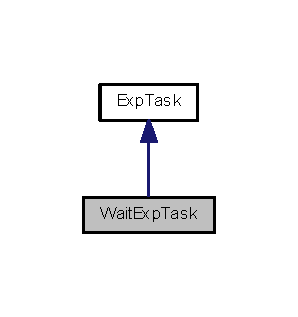
\includegraphics[width=143pt]{class_wait_exp_task__inherit__graph}
\end{center}
\end{figure}
\subsection*{Public Slots}
\begin{DoxyCompactItemize}
\item 
\hypertarget{class_wait_exp_task_a355f9031b6b4cbf0e3b17072fd92e57e}{}virtual void \hyperlink{class_wait_exp_task_a355f9031b6b4cbf0e3b17072fd92e57e}{start} ()\label{class_wait_exp_task_a355f9031b6b4cbf0e3b17072fd92e57e}

\begin{DoxyCompactList}\small\item\em emits \hyperlink{class_wait_exp_task_a0e6b8df7760857ace81f82deb888fb23}{start\+Wait\+Task()} signal, to start waiting for this task and \hyperlink{class_exp_task_aeb51d072a7b96f55da3738a8c7733611}{finished()} signal to finish this task. The waiting for the task is then handled by the \hyperlink{class_waiting_task}{Waiting\+Task}. \end{DoxyCompactList}\item 
\hypertarget{class_wait_exp_task_a7d34d773042648d601c67a5b2c9ee55d}{}virtual void \hyperlink{class_wait_exp_task_a7d34d773042648d601c67a5b2c9ee55d}{stop} ()\label{class_wait_exp_task_a7d34d773042648d601c67a5b2c9ee55d}

\begin{DoxyCompactList}\small\item\em stops adding of the \hyperlink{class_wait_task}{Wait\+Task} to the \hyperlink{class_wait_worker}{Wait\+Worker}. Do not use it. \end{DoxyCompactList}\end{DoxyCompactItemize}
\subsection*{Signals}
\begin{DoxyCompactItemize}
\item 
\hypertarget{class_wait_exp_task_a0e6b8df7760857ace81f82deb888fb23}{}void \hyperlink{class_wait_exp_task_a0e6b8df7760857ace81f82deb888fb23}{start\+Wait\+Task} (unsigned int id)\label{class_wait_exp_task_a0e6b8df7760857ace81f82deb888fb23}

\begin{DoxyCompactList}\small\item\em This signal is emited from the \hyperlink{class_wait_exp_task_a355f9031b6b4cbf0e3b17072fd92e57e}{start()} method, and in \hyperlink{class_wait_task_list}{Wait\+Task\+List} is connected to the \hyperlink{class_wait_task_list_a802528b32bbcacb201bdd5fcfc4dacf6}{Wait\+Task\+List\+::on\+Start\+Wait\+Task()} which submits contained \hyperlink{class_wait_task}{Wait\+Task} to the \hyperlink{class_wait_worker}{Wait\+Worker}. \end{DoxyCompactList}\end{DoxyCompactItemize}
\subsection*{Public Member Functions}
\begin{DoxyCompactItemize}
\item 
\hypertarget{class_wait_exp_task_a15d7409a0fdc6c6da419ad9959c86e71}{}\hyperlink{class_wait_exp_task_a15d7409a0fdc6c6da419ad9959c86e71}{Wait\+Exp\+Task} (const \hyperlink{struct_wait_task_list_traits_1_1_task_item}{Wait\+Task\+List\+Traits\+::\+Task\+Item} \&wait\+Task, Q\+Object $\ast$parent=0)\label{class_wait_exp_task_a15d7409a0fdc6c6da419ad9959c86e71}

\begin{DoxyCompactList}\small\item\em Constructs \hyperlink{class_wait_exp_task}{Wait\+Exp\+Task} object. \end{DoxyCompactList}\item 
\hypertarget{class_wait_exp_task_a8688827b3a1eccec11bdd5d7002ee288}{}virtual \hyperlink{class_wait_exp_task_a8688827b3a1eccec11bdd5d7002ee288}{$\sim$\+Wait\+Exp\+Task} ()\label{class_wait_exp_task_a8688827b3a1eccec11bdd5d7002ee288}

\begin{DoxyCompactList}\small\item\em \hyperlink{class_wait_exp_task_a8688827b3a1eccec11bdd5d7002ee288}{Wait\+Exp\+Task\+::$\sim$\+Wait\+Exp\+Task}. \end{DoxyCompactList}\item 
\hypertarget{class_wait_exp_task_a34d831c5c3497c9e315a5323e9e45b02}{}virtual void \hyperlink{class_wait_exp_task_a34d831c5c3497c9e315a5323e9e45b02}{set\+Delayed\+Delete} (bool bl\+Delayed\+Delete)\label{class_wait_exp_task_a34d831c5c3497c9e315a5323e9e45b02}

\begin{DoxyCompactList}\small\item\em Sets delayed destruction of the task also for the contained \hyperlink{class_wait_task}{Wait\+Task}. Viz \hyperlink{class_exp_task_a2049ca37582a4b3250f3fc46ba19fe2a}{Exp\+Task\+::set\+Delayed\+Delete()} \end{DoxyCompactList}\item 
\hypertarget{class_wait_exp_task_ae9c89cd3011fe082c884fef466317291}{}\hyperlink{struct_wait_task_list_traits_1_1_task_item}{Wait\+Task\+List\+Traits\+::\+Task\+Item} \hyperlink{class_wait_exp_task_ae9c89cd3011fe082c884fef466317291}{get\+Wait\+Task\+Item} ()\label{class_wait_exp_task_ae9c89cd3011fe082c884fef466317291}

\begin{DoxyCompactList}\small\item\em Returns contained \hyperlink{struct_wait_task_list_traits_1_1_task_item}{Wait\+Task\+List\+Traits\+::\+Task\+Item}. This method is used in \hyperlink{class_wait_task_list_a429d0b45f82a2eef00c5dacffbbc1f70}{Wait\+Task\+List\+::add\+Task()}, where the contained \hyperlink{class_wait_task}{Wait\+Task} obtaines its id. \end{DoxyCompactList}\end{DoxyCompactItemize}
\subsection*{Private Attributes}
\begin{DoxyCompactItemize}
\item 
\hypertarget{class_wait_exp_task_a10b668341c30600b359980f4ebecb99f}{}\hyperlink{struct_wait_task_list_traits_1_1_task_item}{Wait\+Task\+List\+Traits\+::\+Task\+Item} \hyperlink{class_wait_exp_task_a10b668341c30600b359980f4ebecb99f}{wait\+Task\+Item}\label{class_wait_exp_task_a10b668341c30600b359980f4ebecb99f}

\begin{DoxyCompactList}\small\item\em contained Wait\+Task\+Item \end{DoxyCompactList}\end{DoxyCompactItemize}


\subsection{Detailed Description}
This class contains the \hyperlink{class_wait_task}{Wait\+Task} in the \hyperlink{struct_wait_task_list_traits_1_1_task_item}{Wait\+Task\+List\+Traits\+::\+Task\+Item}, which will be submited to the list of tasks which will be waited for, when added to the \hyperlink{class_wait_task_list}{Wait\+Task\+List}. Each \hyperlink{class_wait_task}{Wait\+Task} should be handled by some \hyperlink{class_waiting_task}{Waiting\+Task} to have some effect, so there shouldn\textquotesingle{}t be any \hyperlink{class_wait_exp_task}{Wait\+Exp\+Task} added to the \hyperlink{class_wait_task_list}{Wait\+Task\+List} without \hyperlink{class_waiting_task}{Waiting\+Task} added somewhere after it. 

The documentation for this class was generated from the following files\+:\begin{DoxyCompactItemize}
\item 
waittasklist.\+h\item 
waittasklist.\+cpp\end{DoxyCompactItemize}

\hypertarget{class_waiting_task}{}\section{Waiting\+Task Class Reference}
\label{class_waiting_task}\index{Waiting\+Task@{Waiting\+Task}}


Handles waiting for all \hyperlink{class_wait_exp_task}{Wait\+Exp\+Task} objects previously added to the \hyperlink{class_wait_task_list}{Wait\+Task\+List}.  




Inheritance diagram for Waiting\+Task\+:\nopagebreak
\begin{figure}[H]
\begin{center}
\leavevmode
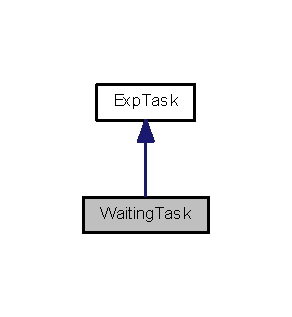
\includegraphics[width=140pt]{class_waiting_task__inherit__graph}
\end{center}
\end{figure}
\subsection*{Public Slots}
\begin{DoxyCompactItemize}
\item 
\hypertarget{class_waiting_task_a93e5b1b87723904e6a4babef1bbd4727}{}void \hyperlink{class_waiting_task_a93e5b1b87723904e6a4babef1bbd4727}{on\+Wait\+Task\+Finished} (unsigned int id)\label{class_waiting_task_a93e5b1b87723904e6a4babef1bbd4727}

\begin{DoxyCompactList}\small\item\em This slot is connected to all \hyperlink{class_wait_task}{Wait\+Task} object, which was added before the addition of this \hyperlink{class_waiting_task}{Waiting\+Task} and not already handled by any preceeding \hyperlink{class_waiting_task}{Waiting\+Task}. It emits \hyperlink{class_waiting_task_a603610acef7edaa2e0e51af6776a18ca}{wait\+Task\+Finished()} signal and if all \hyperlink{class_wait_task}{Wait\+Task} objects which are connected to this \hyperlink{class_waiting_task}{Waiting\+Task} have been already executed, it emits \hyperlink{class_exp_task_aeb51d072a7b96f55da3738a8c7733611}{finished()} signal. \end{DoxyCompactList}\item 
\hypertarget{class_waiting_task_a423901b7576a9eada13609a205da4d12}{}virtual void \hyperlink{class_waiting_task_a423901b7576a9eada13609a205da4d12}{start} ()\label{class_waiting_task_a423901b7576a9eada13609a205da4d12}

\begin{DoxyCompactList}\small\item\em This method starts the waiting for all connected \hyperlink{class_wait_task}{Wait\+Task} objects. See \hyperlink{class_waiting_task_a93e5b1b87723904e6a4babef1bbd4727}{on\+Wait\+Task\+Finished()} slot. \end{DoxyCompactList}\item 
\hypertarget{class_waiting_task_a2bb17c0359c2694e2b8af25c4fce208d}{}virtual void \hyperlink{class_waiting_task_a2bb17c0359c2694e2b8af25c4fce208d}{stop} ()\label{class_waiting_task_a2bb17c0359c2694e2b8af25c4fce208d}

\begin{DoxyCompactList}\small\item\em Stops the waiting. \end{DoxyCompactList}\end{DoxyCompactItemize}
\subsection*{Signals}
\begin{DoxyCompactItemize}
\item 
void \hyperlink{class_waiting_task_a603610acef7edaa2e0e51af6776a18ca}{wait\+Task\+Finished} (unsigned int id)
\begin{DoxyCompactList}\small\item\em This signal is emited from the \hyperlink{class_waiting_task_a93e5b1b87723904e6a4babef1bbd4727}{on\+Wait\+Task\+Finished()} method and connected to the \hyperlink{class_wait_task_list_ab6c3634d0739c8948b028c8db86d804c}{Wait\+Task\+List\+::on\+Wait\+Task\+Finished()} in the \hyperlink{class_wait_task_list_a2724cb9d9e7f897a4bf0c44054ad2c29}{Wait\+Task\+List\+::add\+Wait\+Task()} method which is called from the \hyperlink{class_wait_task_list_a429d0b45f82a2eef00c5dacffbbc1f70}{Wait\+Task\+List\+::add\+Task()} method. \end{DoxyCompactList}\end{DoxyCompactItemize}
\subsection*{Public Member Functions}
\begin{DoxyCompactItemize}
\item 
\hyperlink{class_waiting_task_a806640941e34cbe8fb356404ddb79d82}{Waiting\+Task} (Q\+Object $\ast$parent=0)
\begin{DoxyCompactList}\small\item\em Constructs \hyperlink{class_waiting_task}{Waiting\+Task} object. \end{DoxyCompactList}\item 
\hypertarget{class_waiting_task_a13afb2c5c57743d62345598b47b18f34}{}virtual \hyperlink{class_waiting_task_a13afb2c5c57743d62345598b47b18f34}{$\sim$\+Waiting\+Task} ()\label{class_waiting_task_a13afb2c5c57743d62345598b47b18f34}

\begin{DoxyCompactList}\small\item\em Destoryes \hyperlink{class_waiting_task}{Waiting\+Task} object. \end{DoxyCompactList}\item 
\hypertarget{class_waiting_task_afd06aa0d4a845eaa705f8893cd0d87a3}{}virtual void \hyperlink{class_waiting_task_afd06aa0d4a845eaa705f8893cd0d87a3}{restart\+Times\+Exec} ()\label{class_waiting_task_afd06aa0d4a845eaa705f8893cd0d87a3}

\begin{DoxyCompactList}\small\item\em This method resets the number of planned executions of the \hyperlink{class_waiting_task}{Waiting\+Task} resetting also the \hyperlink{class_wait_task}{Wait\+Task} objects which will be waited for. \end{DoxyCompactList}\item 
void \hyperlink{class_waiting_task_a5123ece4b96ec9229d01d28db64094fa}{set\+Ids} (const Q\+Set$<$ unsigned int $>$ \&ids)
\begin{DoxyCompactList}\small\item\em This method sets the ids of \hyperlink{class_wait_task}{Wait\+Task} objects which will be waited for. It is used in \hyperlink{class_wait_task_list_a2724cb9d9e7f897a4bf0c44054ad2c29}{Wait\+Task\+List\+::add\+Wait\+Task()} method which is called from the \hyperlink{class_wait_task_list_a429d0b45f82a2eef00c5dacffbbc1f70}{Wait\+Task\+List\+::add\+Task()} method. \end{DoxyCompactList}\end{DoxyCompactItemize}
\subsection*{Private Attributes}
\begin{DoxyCompactItemize}
\item 
\hypertarget{class_waiting_task_a7b7e075b8903897855a0dc9e57e34560}{}Q\+Set$<$ unsigned int $>$ \hyperlink{class_waiting_task_a7b7e075b8903897855a0dc9e57e34560}{curr\+Ids\+\_\+}\label{class_waiting_task_a7b7e075b8903897855a0dc9e57e34560}

\begin{DoxyCompactList}\small\item\em Ids of \hyperlink{class_wait_task}{Wait\+Task} object, which are or will be currently waited for. \end{DoxyCompactList}\item 
\hypertarget{class_waiting_task_a707eb238134ae6135b7f5600d49ba39d}{}Q\+Set$<$ unsigned int $>$ \hyperlink{class_waiting_task_a707eb238134ae6135b7f5600d49ba39d}{ids\+\_\+}\label{class_waiting_task_a707eb238134ae6135b7f5600d49ba39d}

\begin{DoxyCompactList}\small\item\em Ids of all \hyperlink{class_wait_task}{Wait\+Task} objects which are connected to this \hyperlink{class_waiting_task}{Waiting\+Task}. \end{DoxyCompactList}\end{DoxyCompactItemize}


\subsection{Detailed Description}
Handles waiting for all \hyperlink{class_wait_exp_task}{Wait\+Exp\+Task} objects previously added to the \hyperlink{class_wait_task_list}{Wait\+Task\+List}. 

\subsection{Constructor \& Destructor Documentation}
\hypertarget{class_waiting_task_a806640941e34cbe8fb356404ddb79d82}{}\index{Waiting\+Task@{Waiting\+Task}!Waiting\+Task@{Waiting\+Task}}
\index{Waiting\+Task@{Waiting\+Task}!Waiting\+Task@{Waiting\+Task}}
\subsubsection[{Waiting\+Task}]{\setlength{\rightskip}{0pt plus 5cm}Waiting\+Task\+::\+Waiting\+Task (
\begin{DoxyParamCaption}
\item[{Q\+Object $\ast$}]{parent = {\ttfamily 0}}
\end{DoxyParamCaption}
)\hspace{0.3cm}{\ttfamily [explicit]}}\label{class_waiting_task_a806640941e34cbe8fb356404ddb79d82}


Constructs \hyperlink{class_waiting_task}{Waiting\+Task} object. 


\begin{DoxyParams}{Parameters}
{\em parent} & Parent Q\+Object in Qt\textquotesingle{}s ownership system. \\
\hline
\end{DoxyParams}


\subsection{Member Function Documentation}
\hypertarget{class_waiting_task_a5123ece4b96ec9229d01d28db64094fa}{}\index{Waiting\+Task@{Waiting\+Task}!set\+Ids@{set\+Ids}}
\index{set\+Ids@{set\+Ids}!Waiting\+Task@{Waiting\+Task}}
\subsubsection[{set\+Ids}]{\setlength{\rightskip}{0pt plus 5cm}Waiting\+Task\+::set\+Ids (
\begin{DoxyParamCaption}
\item[{const Q\+Set$<$ unsigned int $>$ \&}]{ids}
\end{DoxyParamCaption}
)\hspace{0.3cm}{\ttfamily [inline]}}\label{class_waiting_task_a5123ece4b96ec9229d01d28db64094fa}


This method sets the ids of \hyperlink{class_wait_task}{Wait\+Task} objects which will be waited for. It is used in \hyperlink{class_wait_task_list_a2724cb9d9e7f897a4bf0c44054ad2c29}{Wait\+Task\+List\+::add\+Wait\+Task()} method which is called from the \hyperlink{class_wait_task_list_a429d0b45f82a2eef00c5dacffbbc1f70}{Wait\+Task\+List\+::add\+Task()} method. 


\begin{DoxyParams}{Parameters}
{\em ids} & list of ids of tasks which will be waited for. \\
\hline
\end{DoxyParams}
\hypertarget{class_waiting_task_a603610acef7edaa2e0e51af6776a18ca}{}\index{Waiting\+Task@{Waiting\+Task}!wait\+Task\+Finished@{wait\+Task\+Finished}}
\index{wait\+Task\+Finished@{wait\+Task\+Finished}!Waiting\+Task@{Waiting\+Task}}
\subsubsection[{wait\+Task\+Finished}]{\setlength{\rightskip}{0pt plus 5cm}Waiting\+Task\+::wait\+Task\+Finished (
\begin{DoxyParamCaption}
\item[{unsigned int}]{id}
\end{DoxyParamCaption}
)\hspace{0.3cm}{\ttfamily [signal]}}\label{class_waiting_task_a603610acef7edaa2e0e51af6776a18ca}


This signal is emited from the \hyperlink{class_waiting_task_a93e5b1b87723904e6a4babef1bbd4727}{on\+Wait\+Task\+Finished()} method and connected to the \hyperlink{class_wait_task_list_ab6c3634d0739c8948b028c8db86d804c}{Wait\+Task\+List\+::on\+Wait\+Task\+Finished()} in the \hyperlink{class_wait_task_list_a2724cb9d9e7f897a4bf0c44054ad2c29}{Wait\+Task\+List\+::add\+Wait\+Task()} method which is called from the \hyperlink{class_wait_task_list_a429d0b45f82a2eef00c5dacffbbc1f70}{Wait\+Task\+List\+::add\+Task()} method. 


\begin{DoxyParams}{Parameters}
{\em id} & of finished \hyperlink{class_wait_task}{Wait\+Task} \\
\hline
\end{DoxyParams}


The documentation for this class was generated from the following files\+:\begin{DoxyCompactItemize}
\item 
waittasklist.\+h\item 
waittasklist.\+cpp\end{DoxyCompactItemize}

\hypertarget{class_wait_task}{}\section{Wait\+Task Class Reference}
\label{class_wait_task}\index{Wait\+Task@{Wait\+Task}}


Abstract class which forms the base for task usable with \hyperlink{class_wait_task_list}{Wait\+Task\+List}. The \hyperlink{class_wait_task_a39f09592449c61469d093f980a23cbfd}{running()} method need to be reimplemented.  




Inherits Q\+Object.



Inherited by Delay\+Wait\+Task, Stage\+Control\+Wait\+Task, and Win\+Spec\+Wait\+Task.

\subsection*{Public Slots}
\begin{DoxyCompactItemize}
\item 
\hypertarget{class_wait_task_ab20934c4c6723db758564eef74eec5c4}{}virtual void \hyperlink{class_wait_task_ab20934c4c6723db758564eef74eec5c4}{start} ()\label{class_wait_task_ab20934c4c6723db758564eef74eec5c4}

\begin{DoxyCompactList}\small\item\em Contains commands which is executed at the beginning of the waiting. \end{DoxyCompactList}\item 
\hypertarget{class_wait_task_a6bbc82bd62e9fc2cad789a24a6ab928a}{}virtual void \hyperlink{class_wait_task_a6bbc82bd62e9fc2cad789a24a6ab928a}{stop} ()\label{class_wait_task_a6bbc82bd62e9fc2cad789a24a6ab928a}

\begin{DoxyCompactList}\small\item\em Contains commands which is executed when the waiting is stopped. It emits \hyperlink{class_wait_task_a224392dd1ee8414b1bdb54619c45f001}{waiting\+Failed()} signal and calls \hyperlink{class_wait_task_a5f3a89b190e0ef7443cc3b9cc8857e9a}{finish()} method. \end{DoxyCompactList}\item 
\hypertarget{class_wait_task_a5f3a89b190e0ef7443cc3b9cc8857e9a}{}virtual void \hyperlink{class_wait_task_a5f3a89b190e0ef7443cc3b9cc8857e9a}{finish} ()\label{class_wait_task_a5f3a89b190e0ef7443cc3b9cc8857e9a}

\begin{DoxyCompactList}\small\item\em Contains commands which is executed when the waiting is finished and emits \hyperlink{class_wait_task_ae52cf854c36339a1cad9c643e6259978}{wait\+Task\+Finished()} signal. \end{DoxyCompactList}\end{DoxyCompactItemize}
\subsection*{Signals}
\begin{DoxyCompactItemize}
\item 
\hypertarget{class_wait_task_ae52cf854c36339a1cad9c643e6259978}{}void \hyperlink{class_wait_task_ae52cf854c36339a1cad9c643e6259978}{wait\+Task\+Finished} (unsigned int uint\+Id)\label{class_wait_task_ae52cf854c36339a1cad9c643e6259978}

\begin{DoxyCompactList}\small\item\em This signal need to be emited after the execution of the \hyperlink{class_wait_task}{Wait\+Task} is finished (succesfully or not) to stop waiting for this \hyperlink{class_wait_task}{Wait\+Task}. It is emited from \hyperlink{class_wait_task_a5f3a89b190e0ef7443cc3b9cc8857e9a}{Wait\+Task\+::finish()} method. \end{DoxyCompactList}\item 
\hypertarget{class_wait_task_a224392dd1ee8414b1bdb54619c45f001}{}void \hyperlink{class_wait_task_a224392dd1ee8414b1bdb54619c45f001}{waiting\+Failed} ()\label{class_wait_task_a224392dd1ee8414b1bdb54619c45f001}

\begin{DoxyCompactList}\small\item\em This signal is emited when the waiting for this wait task is stopped from the \hyperlink{class_wait_task_a6bbc82bd62e9fc2cad789a24a6ab928a}{Wait\+Task\+::stop()} method. \end{DoxyCompactList}\end{DoxyCompactItemize}
\subsection*{Public Member Functions}
\begin{DoxyCompactItemize}
\item 
\hyperlink{class_wait_task_ac439dd31c2e1d6fc1df3328fa9b30a68}{Wait\+Task} (Q\+Object $\ast$parent=0)
\begin{DoxyCompactList}\small\item\em Constructs \hyperlink{class_wait_task}{Wait\+Task} object. \end{DoxyCompactList}\item 
\hypertarget{class_wait_task_ae5b9cca0e1b394f23f82d7ef5bd3a517}{}virtual \hyperlink{class_wait_task_ae5b9cca0e1b394f23f82d7ef5bd3a517}{$\sim$\+Wait\+Task} ()\label{class_wait_task_ae5b9cca0e1b394f23f82d7ef5bd3a517}

\begin{DoxyCompactList}\small\item\em Destroyes the \hyperlink{class_wait_task}{Wait\+Task}. \end{DoxyCompactList}\item 
\hypertarget{class_wait_task_a39f09592449c61469d093f980a23cbfd}{}virtual bool \hyperlink{class_wait_task_a39f09592449c61469d093f980a23cbfd}{running} ()=0\label{class_wait_task_a39f09592449c61469d093f980a23cbfd}

\begin{DoxyCompactList}\small\item\em Virtual method, which need to be reimplemented. If this method returns false, the waiting in \hyperlink{class_wait_task_list}{Wait\+Task\+List} is ended. \end{DoxyCompactList}\item 
\hypertarget{class_wait_task_a3984ae37eae1a984db2f2417df2bfbbf}{}int \hyperlink{class_wait_task_a3984ae37eae1a984db2f2417df2bfbbf}{initial\+Delay} () const \label{class_wait_task_a3984ae37eae1a984db2f2417df2bfbbf}

\begin{DoxyCompactList}\small\item\em Returns initial delay. See the class description for more details. \end{DoxyCompactList}\item 
\hypertarget{class_wait_task_a151808251a297dec52be3d6713eaaf1d}{}bool \hyperlink{class_wait_task_a151808251a297dec52be3d6713eaaf1d}{delayed\+Delete} () const \label{class_wait_task_a151808251a297dec52be3d6713eaaf1d}

\begin{DoxyCompactList}\small\item\em This method returns true if the deletion of the \hyperlink{class_wait_task}{Wait\+Task} may be delayed. See \hyperlink{class_wait_task_a2d90e1b45c8218c8fab89b5adb2dcaae}{set\+Delayed\+Delete()} for more details. \end{DoxyCompactList}\item 
\hypertarget{class_wait_task_a060f5d982d06d90546ca7a23518d09e0}{}unsigned int \hyperlink{class_wait_task_a060f5d982d06d90546ca7a23518d09e0}{id} () const \label{class_wait_task_a060f5d982d06d90546ca7a23518d09e0}

\begin{DoxyCompactList}\small\item\em Gets \hyperlink{class_wait_task}{Wait\+Task}\textquotesingle{}s id. This id is retreived in \hyperlink{class_wait_task_list}{Wait\+Task\+List}\textquotesingle{}s id system. \end{DoxyCompactList}\item 
\hypertarget{class_wait_task_a34687474d76ecdc799c31cf7fd49e01f}{}bool \hyperlink{class_wait_task_a34687474d76ecdc799c31cf7fd49e01f}{handled} () const \label{class_wait_task_a34687474d76ecdc799c31cf7fd49e01f}

\begin{DoxyCompactList}\small\item\em True, if \hyperlink{class_wait_task}{Wait\+Task} is handled by some \hyperlink{class_waiting_task}{Waiting\+Task} in \hyperlink{class_wait_task_list}{Wait\+Task\+List}. \end{DoxyCompactList}\item 
\hypertarget{class_wait_task_aa142fbaa9a075defd892f516083af4b7}{}void \hyperlink{class_wait_task_aa142fbaa9a075defd892f516083af4b7}{set\+Initial\+Delay} (int init\+Delay)\label{class_wait_task_aa142fbaa9a075defd892f516083af4b7}

\begin{DoxyCompactList}\small\item\em Sets initial delay in ms before the waiting in \hyperlink{class_wait_task_list}{Wait\+Task\+List} begins. \end{DoxyCompactList}\item 
\hypertarget{class_wait_task_a2d90e1b45c8218c8fab89b5adb2dcaae}{}void \hyperlink{class_wait_task_a2d90e1b45c8218c8fab89b5adb2dcaae}{set\+Delayed\+Delete} (bool bl\+Delayed\+Delete)\label{class_wait_task_a2d90e1b45c8218c8fab89b5adb2dcaae}

\begin{DoxyCompactList}\small\item\em This method sets the if the \hyperlink{class_wait_task}{Wait\+Task} will be deleted immediatelly after it is finished or not. The delayed deletion is necessary in the case when the \hyperlink{class_waiting_task}{Waiting\+Task} which waits for this \hyperlink{class_wait_task}{Wait\+Task} will be executed repetitively. For the details see \hyperlink{class_exp_task_a2049ca37582a4b3250f3fc46ba19fe2a}{Exp\+Task\+::set\+Delayed\+Delete()} \end{DoxyCompactList}\item 
\hypertarget{class_wait_task_a25ff7bb1e0dee67244f6336e21840b18}{}void \hyperlink{class_wait_task_a25ff7bb1e0dee67244f6336e21840b18}{set\+Id} (unsigned int uint\+Id)\label{class_wait_task_a25ff7bb1e0dee67244f6336e21840b18}

\begin{DoxyCompactList}\small\item\em Sets the \hyperlink{class_wait_task}{Wait\+Task}\textquotesingle{}s id. This methods is used by the \hyperlink{class_wait_task_list}{Wait\+Task\+List} to manage contained \hyperlink{class_wait_task}{Wait\+Task} objects. \end{DoxyCompactList}\item 
\hypertarget{class_wait_task_ae128632bbf239153c64a5ba968643747}{}void \hyperlink{class_wait_task_ae128632bbf239153c64a5ba968643747}{set\+Handled} (bool bl\+Handled)\label{class_wait_task_ae128632bbf239153c64a5ba968643747}

\begin{DoxyCompactList}\small\item\em Sets if the \hyperlink{class_wait_task}{Wait\+Task} is handled by some \hyperlink{class_waiting_task}{Waiting\+Task} or not. If it is not handled in the time it may be executed in \hyperlink{class_wait_task_list}{Wait\+Task\+List}, the execution of this task is skipped. \end{DoxyCompactList}\end{DoxyCompactItemize}
\subsection*{Private Attributes}
\begin{DoxyCompactItemize}
\item 
\hypertarget{class_wait_task_a0dcba6c8771739ede9d99fe2ec797536}{}unsigned int \hyperlink{class_wait_task_a0dcba6c8771739ede9d99fe2ec797536}{id\+\_\+}\label{class_wait_task_a0dcba6c8771739ede9d99fe2ec797536}

\begin{DoxyCompactList}\small\item\em id of the \hyperlink{class_wait_task}{Wait\+Task}, which was retreived from the \hyperlink{class_wait_task_list}{Wait\+Task\+List} id system. \end{DoxyCompactList}\item 
\hypertarget{class_wait_task_a37036e5f62e2edcdf7ae6e98d221aa64}{}int \hyperlink{class_wait_task_a37036e5f62e2edcdf7ae6e98d221aa64}{init\+Delay\+\_\+}\label{class_wait_task_a37036e5f62e2edcdf7ae6e98d221aa64}

\begin{DoxyCompactList}\small\item\em initial delay in ms which is waited before the waiting for \hyperlink{class_wait_task}{Wait\+Task} is proceeded. \end{DoxyCompactList}\item 
\hypertarget{class_wait_task_aaac2268db578ccf6ec74b1ab07c2bf04}{}bool \hyperlink{class_wait_task_aaac2268db578ccf6ec74b1ab07c2bf04}{bl\+Delayed\+Delete\+\_\+}\label{class_wait_task_aaac2268db578ccf6ec74b1ab07c2bf04}

\begin{DoxyCompactList}\small\item\em true if the \hyperlink{class_wait_task}{Wait\+Task} should not be deleted immediatelly after it finishes. \end{DoxyCompactList}\item 
\hypertarget{class_wait_task_a3c01a70426e88f4ce098533c2029db7e}{}Q\+Mutex $\ast$ \hyperlink{class_wait_task_a3c01a70426e88f4ce098533c2029db7e}{delayed\+Delete\+Mutex}\label{class_wait_task_a3c01a70426e88f4ce098533c2029db7e}

\begin{DoxyCompactList}\small\item\em mutex which manages thread safety. \end{DoxyCompactList}\item 
\hypertarget{class_wait_task_a9af35161099d8dbc938dfc6a00541ca0}{}bool \hyperlink{class_wait_task_a9af35161099d8dbc938dfc6a00541ca0}{handled\+\_\+}\label{class_wait_task_a9af35161099d8dbc938dfc6a00541ca0}

\begin{DoxyCompactList}\small\item\em true if the \hyperlink{class_wait_task}{Wait\+Task} is handled by some \hyperlink{class_waiting_task}{Waiting\+Task} in \hyperlink{class_wait_task_list}{Wait\+Task\+List}. \end{DoxyCompactList}\end{DoxyCompactItemize}


\subsection{Detailed Description}
Abstract class which forms the base for task usable with \hyperlink{class_wait_task_list}{Wait\+Task\+List}. The \hyperlink{class_wait_task_a39f09592449c61469d093f980a23cbfd}{running()} method need to be reimplemented. 

The object of this class is added wrapped in the Wait\+Task\+List\+Tratis\+::\+Task\+Item to the \hyperlink{class_wait_exp_task}{Wait\+Exp\+Task} and when the \hyperlink{class_wait_exp_task}{Wait\+Exp\+Task} is added to the \hyperlink{class_wait_task_list}{Wait\+Task\+List}, it is submited to the list of \hyperlink{class_wait_task}{Wait\+Task} objects. Then, when \hyperlink{class_waiting_task}{Waiting\+Task} is added, the \hyperlink{class_wait_task}{Wait\+Task}\textquotesingle{}s \hyperlink{class_wait_task_ae52cf854c36339a1cad9c643e6259978}{wait\+Task\+Finished()} signal is connected to the \hyperlink{class_waiting_task}{Waiting\+Task}\textquotesingle{}s \hyperlink{class_waiting_task_a93e5b1b87723904e6a4babef1bbd4727}{Waiting\+Task\+::on\+Wait\+Task\+Finished()} slot. The, if the \hyperlink{class_wait_exp_task}{Wait\+Exp\+Task} is started in the \hyperlink{class_wait_task_list}{Wait\+Task\+List}, the \hyperlink{class_wait_worker}{Wait\+Worker} controlls if \hyperlink{class_wait_task_a3984ae37eae1a984db2f2417df2bfbbf}{initial\+Delay()} is greater than zero and if so, it waits at first the initial delay, then it calls \hyperlink{class_wait_task}{Wait\+Task}\textquotesingle{}s \hyperlink{class_wait_task_ab20934c4c6723db758564eef74eec5c4}{start()} method and then periodically controlls the \hyperlink{class_wait_task_a39f09592449c61469d093f980a23cbfd}{running()} method and when it returns false, the \hyperlink{class_wait_task}{Wait\+Task}\textquotesingle{}s \hyperlink{class_wait_task_a5f3a89b190e0ef7443cc3b9cc8857e9a}{finish()} method is called which should emit the \hyperlink{class_wait_task_ae52cf854c36339a1cad9c643e6259978}{wait\+Task\+Finished()} signal at the end. 

\subsection{Constructor \& Destructor Documentation}
\hypertarget{class_wait_task_ac439dd31c2e1d6fc1df3328fa9b30a68}{}\index{Wait\+Task@{Wait\+Task}!Wait\+Task@{Wait\+Task}}
\index{Wait\+Task@{Wait\+Task}!Wait\+Task@{Wait\+Task}}
\subsubsection[{Wait\+Task}]{\setlength{\rightskip}{0pt plus 5cm}Wait\+Task\+::\+Wait\+Task (
\begin{DoxyParamCaption}
\item[{Q\+Object $\ast$}]{parent = {\ttfamily 0}}
\end{DoxyParamCaption}
)\hspace{0.3cm}{\ttfamily [explicit]}}\label{class_wait_task_ac439dd31c2e1d6fc1df3328fa9b30a68}


Constructs \hyperlink{class_wait_task}{Wait\+Task} object. 


\begin{DoxyParams}{Parameters}
{\em parent} & Parent in Qt\textquotesingle{}s ownership system. \\
\hline
\end{DoxyParams}


The documentation for this class was generated from the following files\+:\begin{DoxyCompactItemize}
\item 
waittask.\+h\item 
waittask.\+cpp\end{DoxyCompactItemize}

\hypertarget{class_wait_task_list}{}\section{Wait\+Task\+List Class Reference}
\label{class_wait_task_list}\index{Wait\+Task\+List@{Wait\+Task\+List}}


This class provides interface for executing tasks which waits for some process to be finished.  




Inheritance diagram for Wait\+Task\+List\+:\nopagebreak
\begin{figure}[H]
\begin{center}
\leavevmode
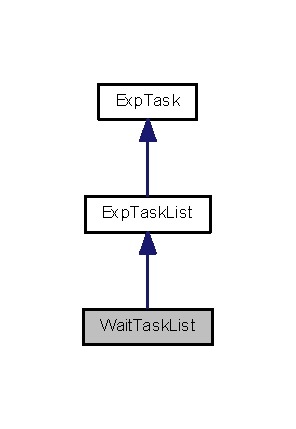
\includegraphics[width=142pt]{class_wait_task_list__inherit__graph}
\end{center}
\end{figure}
\subsection*{Public Slots}
\begin{DoxyCompactItemize}
\item 
\hypertarget{class_wait_task_list_a991a520e472601b7c4457035c22c4c22}{}virtual void \hyperlink{class_wait_task_list_a991a520e472601b7c4457035c22c4c22}{start} ()\label{class_wait_task_list_a991a520e472601b7c4457035c22c4c22}

\begin{DoxyCompactList}\small\item\em Starts execution of the \hyperlink{class_exp_task}{Exp\+Task} objects in \hyperlink{class_wait_task_list}{Wait\+Task\+List} and builds the new thread, which can execute all \hyperlink{class_wait_task}{Wait\+Task}\textquotesingle{}s which are wrapped in the \hyperlink{class_wait_exp_task}{Wait\+Exp\+Task} objects inserted in the \hyperlink{class_wait_task_list}{Wait\+Task\+List}. The execution can be stopped by the \hyperlink{class_wait_task_list_acffb5d311033d065e2b5889a0c51f3f1}{stop()} method. See \hyperlink{class_wait_task_list_a429d0b45f82a2eef00c5dacffbbc1f70}{add\+Task()} for more details. \end{DoxyCompactList}\item 
\hypertarget{class_wait_task_list_acffb5d311033d065e2b5889a0c51f3f1}{}virtual void \hyperlink{class_wait_task_list_acffb5d311033d065e2b5889a0c51f3f1}{stop} ()\label{class_wait_task_list_acffb5d311033d065e2b5889a0c51f3f1}

\begin{DoxyCompactList}\small\item\em Stops the \hyperlink{class_wait_task_list}{Wait\+Task\+List} execution. \end{DoxyCompactList}\item 
void \hyperlink{class_wait_task_list_a802528b32bbcacb201bdd5fcfc4dacf6}{on\+Start\+Wait\+Task} (unsigned int id)
\begin{DoxyCompactList}\small\item\em This slot is connected to \hyperlink{class_wait_exp_task_a0e6b8df7760857ace81f82deb888fb23}{Wait\+Exp\+Task\+::start\+Wait\+Task()} signals of the all contained \hyperlink{class_wait_exp_task}{Wait\+Exp\+Task} objects and if the corresponding \hyperlink{class_wait_task}{Wait\+Task} is handled by some \hyperlink{class_waiting_task}{Waiting\+Task}, it is added to the \hyperlink{class_wait_worker}{Wait\+Worker} to be waited for. \end{DoxyCompactList}\item 
void \hyperlink{class_wait_task_list_ab6c3634d0739c8948b028c8db86d804c}{on\+Wait\+Task\+Finished} (unsigned int id)
\begin{DoxyCompactList}\small\item\em This slot is connected to the \hyperlink{class_waiting_task_a603610acef7edaa2e0e51af6776a18ca}{Waiting\+Task\+::wait\+Task\+Finished()} signal which is emited from the current running \hyperlink{class_waiting_task_a93e5b1b87723904e6a4babef1bbd4727}{Waiting\+Task\+::on\+Wait\+Task\+Finished()} slot connected to the \hyperlink{class_wait_task_ae52cf854c36339a1cad9c643e6259978}{Wait\+Task\+::wait\+Task\+Finished()} signal of the currently executed \hyperlink{class_wait_task}{Wait\+Task} objects. \end{DoxyCompactList}\item 
void \hyperlink{class_wait_task_list_acb4be74c64bd3df403657f625384f453}{on\+Worker\+Quit\+Finished} ()
\begin{DoxyCompactList}\small\item\em This method is invoked only when the thread was quited by calling wait\+Worker\textquotesingle{}s \hyperlink{class_wait_worker_af01864effa7662c8261128ff12fb922d}{Wait\+Worker\+::stop()} method in a reaction to the \hyperlink{class_wait_worker_a5f65bc5e4691e9542afef8df55bf27be}{Wait\+Worker\+::quit\+Finished()} signal. \end{DoxyCompactList}\end{DoxyCompactItemize}
\subsection*{Signals}
\begin{DoxyCompactItemize}
\item 
\hypertarget{class_wait_task_list_a1a0af6e55c2eca825e8c31f0ace72305}{}void \hyperlink{class_wait_task_list_a1a0af6e55c2eca825e8c31f0ace72305}{start\+Wait\+Task\+In\+Worker} (\hyperlink{struct_wait_task_list_traits_1_1_task_item}{Wait\+Task\+List\+Traits\+::\+Task\+Item} wait\+Task\+Item)\label{class_wait_task_list_a1a0af6e55c2eca825e8c31f0ace72305}

\begin{DoxyCompactList}\small\item\em Emitted from the \hyperlink{class_wait_task_list_a802528b32bbcacb201bdd5fcfc4dacf6}{on\+Start\+Wait\+Task()} method and connected to the \hyperlink{class_wait_task_list_a35a7c23d4a05850df13e3f8f565c2ba0}{Wait\+Task\+List\+::wait\+Worker}\textquotesingle{}s \hyperlink{class_wait_worker_adaff9ea88795fa9d902711c1952828cd}{Wait\+Worker\+::add\+Wait\+Task()} slot. \end{DoxyCompactList}\item 
\hypertarget{class_wait_task_list_a2839e0820f114d0d8e3509aa9b9a8688}{}void \hyperlink{class_wait_task_list_a2839e0820f114d0d8e3509aa9b9a8688}{stop\+Worker} ()\label{class_wait_task_list_a2839e0820f114d0d8e3509aa9b9a8688}

\begin{DoxyCompactList}\small\item\em Emitted from the \hyperlink{class_wait_task_list_acffb5d311033d065e2b5889a0c51f3f1}{stop()} slot and from the destructor, to stop \hyperlink{class_wait_worker}{Wait\+Worker}. It is connected to the \hyperlink{class_wait_worker}{Wait\+Worker}\textquotesingle{}s \hyperlink{class_wait_worker_af01864effa7662c8261128ff12fb922d}{Wait\+Worker\+::stop()} slot. \end{DoxyCompactList}\end{DoxyCompactItemize}
\subsection*{Public Member Functions}
\begin{DoxyCompactItemize}
\item 
\hyperlink{class_wait_task_list_a2d8cb0fef4e72ba726ed5abf11068a0c}{Wait\+Task\+List} (Q\+Object $\ast$parent=0)
\begin{DoxyCompactList}\small\item\em Creates \hyperlink{class_wait_task_list}{Wait\+Task\+List} object. \end{DoxyCompactList}\item 
\hypertarget{class_wait_task_list_a1ee55fa11961eb48fc27fd43315d6b89}{}\hyperlink{class_wait_task_list_a1ee55fa11961eb48fc27fd43315d6b89}{$\sim$\+Wait\+Task\+List} ()\label{class_wait_task_list_a1ee55fa11961eb48fc27fd43315d6b89}

\begin{DoxyCompactList}\small\item\em Destroyes \hyperlink{class_wait_task_list}{Wait\+Task\+List}. \end{DoxyCompactList}\item 
\hypertarget{class_wait_task_list_a429d0b45f82a2eef00c5dacffbbc1f70}{}virtual void \hyperlink{class_wait_task_list_a429d0b45f82a2eef00c5dacffbbc1f70}{add\+Task} (\hyperlink{struct_exp_task_list_traits_1_1_task_item}{Exp\+Task\+List\+Traits\+::\+Task\+Item} tsk)\label{class_wait_task_list_a429d0b45f82a2eef00c5dacffbbc1f70}

\begin{DoxyCompactList}\small\item\em Adds task to the list and calls the \hyperlink{class_wait_task_list_a2724cb9d9e7f897a4bf0c44054ad2c29}{add\+Wait\+Task()} method, which treats the special cases connected to the handling of \hyperlink{class_wait_task}{Wait\+Task} objects. \end{DoxyCompactList}\item 
\hypertarget{class_wait_task_list_a58f0968b5170d579493176a695c72f8d}{}bool \hyperlink{class_wait_task_list_a58f0968b5170d579493176a695c72f8d}{quit} ()\label{class_wait_task_list_a58f0968b5170d579493176a695c72f8d}

\begin{DoxyCompactList}\small\item\em returns true if \hyperlink{class_wait_task_list_a9757db554cd87cd191cc126a2d5c83cd}{set\+Quit()} was set to true. \end{DoxyCompactList}\item 
\hypertarget{class_wait_task_list_a99ded3b20e08230ebd46dd9fe56d2cfd}{}bool \hyperlink{class_wait_task_list_a99ded3b20e08230ebd46dd9fe56d2cfd}{task\+List\+Is\+Finished} ()\label{class_wait_task_list_a99ded3b20e08230ebd46dd9fe56d2cfd}

\begin{DoxyCompactList}\small\item\em returns true if \hyperlink{class_wait_task_list_a5ff4ac32cdc30ec81775c02f4bd789b6}{set\+Task\+List\+Finished()} was set to true. \end{DoxyCompactList}\item 
\hypertarget{class_wait_task_list_a17ebed288354da92096e21d9411b4c7e}{}bool \hyperlink{class_wait_task_list_a17ebed288354da92096e21d9411b4c7e}{wait\+Worker\+Is\+Finished} ()\label{class_wait_task_list_a17ebed288354da92096e21d9411b4c7e}

\begin{DoxyCompactList}\small\item\em returns true if \hyperlink{class_wait_task_list_a6e5bf6d4151a3ea609db423e1b138310}{set\+Wait\+Worker\+Finished()} was set to true. \end{DoxyCompactList}\item 
\hypertarget{class_wait_task_list_a9757db554cd87cd191cc126a2d5c83cd}{}void \hyperlink{class_wait_task_list_a9757db554cd87cd191cc126a2d5c83cd}{set\+Quit} (bool bl\+Quit)\label{class_wait_task_list_a9757db554cd87cd191cc126a2d5c83cd}

\begin{DoxyCompactList}\small\item\em \hyperlink{class_wait_task_list_a9757db554cd87cd191cc126a2d5c83cd}{set\+Quit()} \end{DoxyCompactList}\item 
\hypertarget{class_wait_task_list_a5ff4ac32cdc30ec81775c02f4bd789b6}{}void \hyperlink{class_wait_task_list_a5ff4ac32cdc30ec81775c02f4bd789b6}{set\+Task\+List\+Finished} (bool bl\+Task\+List\+Finished)\label{class_wait_task_list_a5ff4ac32cdc30ec81775c02f4bd789b6}

\begin{DoxyCompactList}\small\item\em \hyperlink{class_wait_task_list_a5ff4ac32cdc30ec81775c02f4bd789b6}{set\+Task\+List\+Finished()} \end{DoxyCompactList}\item 
\hypertarget{class_wait_task_list_a6e5bf6d4151a3ea609db423e1b138310}{}void \hyperlink{class_wait_task_list_a6e5bf6d4151a3ea609db423e1b138310}{set\+Wait\+Worker\+Finished} (bool bl\+Wait\+Worker\+Finished)\label{class_wait_task_list_a6e5bf6d4151a3ea609db423e1b138310}

\begin{DoxyCompactList}\small\item\em \hyperlink{class_wait_task_list_a6e5bf6d4151a3ea609db423e1b138310}{set\+Wait\+Worker\+Finished()} \end{DoxyCompactList}\end{DoxyCompactItemize}
\subsection*{Protected Member Functions}
\begin{DoxyCompactItemize}
\item 
virtual void \hyperlink{class_wait_task_list_aa0749dc369379ff737fdf14a89142bd2}{task\+List\+Finished} ()
\begin{DoxyCompactList}\small\item\em This is reimplemented method of the \hyperlink{class_exp_task_list_adee3f2e0894b5b102b2fcf0cff4ff25a}{Exp\+Task\+List\+::task\+List\+Finished()}. \end{DoxyCompactList}\item 
void \hyperlink{class_wait_task_list_a2724cb9d9e7f897a4bf0c44054ad2c29}{add\+Wait\+Task} (const \hyperlink{struct_exp_task_list_traits_1_1_task_item}{Exp\+Task\+List\+Traits\+::\+Task\+Item} \&tsk, Q\+Set$<$ unsigned int $>$ $\ast$curr\+New\+Ids=0)
\begin{DoxyCompactList}\small\item\em This method is called from \hyperlink{class_wait_task_list_a429d0b45f82a2eef00c5dacffbbc1f70}{add\+Task()} to controll, if new added task is not a case which requires special treatment (\hyperlink{class_wait_exp_task}{Wait\+Exp\+Task}, \hyperlink{class_waiting_task}{Waiting\+Task}, \hyperlink{class_exp_task_list}{Exp\+Task\+List}, \hyperlink{class_fork_join_task}{Fork\+Join\+Task}). See description of the class for more details. \end{DoxyCompactList}\end{DoxyCompactItemize}
\subsection*{Private Member Functions}
\begin{DoxyCompactItemize}
\item 
unsigned int \hyperlink{class_wait_task_list_a6d38013814172b4f3de755b455e2230e}{get\+Id} ()
\begin{DoxyCompactList}\small\item\em Gets unused id for \hyperlink{class_wait_task_list}{Wait\+Task\+List}\textquotesingle{}s \hyperlink{class_wait_task}{Wait\+Task} id system. \end{DoxyCompactList}\item 
\hypertarget{class_wait_task_list_ad912d65f84926ef852531a261d9e33f4}{}void \hyperlink{class_wait_task_list_ad912d65f84926ef852531a261d9e33f4}{build\+Thread} ()\label{class_wait_task_list_ad912d65f84926ef852531a261d9e33f4}

\begin{DoxyCompactList}\small\item\em Constructs a new Q\+Thread and connects the \hyperlink{class_wait_task_list_a2839e0820f114d0d8e3509aa9b9a8688}{Wait\+Task\+List\+::stop\+Worker()} signal to the \hyperlink{class_wait_worker_af01864effa7662c8261128ff12fb922d}{Wait\+Worker\+::stop()}, \hyperlink{class_wait_task_list_a1a0af6e55c2eca825e8c31f0ace72305}{Wait\+Task\+List\+::start\+Wait\+Task\+In\+Worker()} signal to the \hyperlink{class_wait_worker_adaff9ea88795fa9d902711c1952828cd}{Wait\+Worker\+::add\+Wait\+Task()} and finally \hyperlink{class_wait_worker_a5f65bc5e4691e9542afef8df55bf27be}{Wait\+Worker\+::quit\+Finished()} signal to the \hyperlink{class_wait_task_list_acb4be74c64bd3df403657f625384f453}{Wait\+Task\+List\+::on\+Worker\+Quit\+Finished()} slot. Then it starts thread. \end{DoxyCompactList}\end{DoxyCompactItemize}
\subsection*{Private Attributes}
\begin{DoxyCompactItemize}
\item 
Q\+Thread $\ast$ \hyperlink{class_wait_task_list_a853a1390df826723ab93a21b06cb6c30}{thread}
\begin{DoxyCompactList}\small\item\em The Q\+Thread object, which contains thread in which the \hyperlink{class_wait_worker}{Wait\+Worker} object runs. \end{DoxyCompactList}\item 
\hypertarget{class_wait_task_list_a35a7c23d4a05850df13e3f8f565c2ba0}{}\hyperlink{class_wait_worker}{Wait\+Worker} $\ast$ \hyperlink{class_wait_task_list_a35a7c23d4a05850df13e3f8f565c2ba0}{wait\+Worker}\label{class_wait_task_list_a35a7c23d4a05850df13e3f8f565c2ba0}

\begin{DoxyCompactList}\small\item\em The \hyperlink{class_wait_worker}{Wait\+Worker} object, which controlls wheather the contained \hyperlink{class_wait_task}{Wait\+Task}\textquotesingle{}s is running. \end{DoxyCompactList}\item 
\hypertarget{class_wait_task_list_a70ccd79d9ce35e704cafd37a57d8cc42}{}Q\+Map$<$ unsigned int, \hyperlink{struct_wait_task_list_traits_1_1_task_item}{Wait\+Task\+List\+Traits\+::\+Task\+Item} $>$ \hyperlink{class_wait_task_list_a70ccd79d9ce35e704cafd37a57d8cc42}{wait\+Tasks}\label{class_wait_task_list_a70ccd79d9ce35e704cafd37a57d8cc42}

\begin{DoxyCompactList}\small\item\em List which contains all the added \hyperlink{class_wait_task}{Wait\+Task} objects and their ids. \end{DoxyCompactList}\item 
\hypertarget{class_wait_task_list_a8c562a3ce5414dd19a4d088a01e864ad}{}Q\+Set$<$ unsigned int $>$ \hyperlink{class_wait_task_list_a8c562a3ce5414dd19a4d088a01e864ad}{new\+Ids}\label{class_wait_task_list_a8c562a3ce5414dd19a4d088a01e864ad}

\begin{DoxyCompactList}\small\item\em List containing ids of \hyperlink{class_wait_task}{Wait\+Task} objects which have not aready been handle by some \hyperlink{class_waiting_task}{Waiting\+Task}. \end{DoxyCompactList}\item 
\hypertarget{class_wait_task_list_a35a6d69e8a0d0799bcb08220f7452d87}{}bool \hyperlink{class_wait_task_list_a35a6d69e8a0d0799bcb08220f7452d87}{bl\+Quit\+\_\+}\label{class_wait_task_list_a35a6d69e8a0d0799bcb08220f7452d87}

\begin{DoxyCompactList}\small\item\em Indicitas, if the execution of \hyperlink{class_wait_task_list}{Wait\+Task\+List} was stopped by the \hyperlink{class_wait_task_list_acffb5d311033d065e2b5889a0c51f3f1}{stop()} method. \end{DoxyCompactList}\item 
\hypertarget{class_wait_task_list_a50d68d7fddb9cbdc87e9c566f10ee14e}{}bool \hyperlink{class_wait_task_list_a50d68d7fddb9cbdc87e9c566f10ee14e}{bl\+Task\+List\+Finished\+\_\+}\label{class_wait_task_list_a50d68d7fddb9cbdc87e9c566f10ee14e}

\begin{DoxyCompactList}\small\item\em Indicates, if the \hyperlink{class_exp_task_list}{Exp\+Task\+List} object inside the \hyperlink{class_wait_task_list}{Wait\+Task\+List} has already finished when the \hyperlink{class_wait_task_list_acffb5d311033d065e2b5889a0c51f3f1}{stop()} method was invoked. \end{DoxyCompactList}\item 
\hypertarget{class_wait_task_list_a7c776c15701ac7f1486b392db78a5cec}{}bool \hyperlink{class_wait_task_list_a7c776c15701ac7f1486b392db78a5cec}{bl\+Wait\+Worker\+Finished\+\_\+}\label{class_wait_task_list_a7c776c15701ac7f1486b392db78a5cec}

\begin{DoxyCompactList}\small\item\em Indicates, if the wait\+Worker has already finished when the \hyperlink{class_wait_task_list_acffb5d311033d065e2b5889a0c51f3f1}{stop()} method was invoked. \end{DoxyCompactList}\end{DoxyCompactItemize}
\subsection*{Additional Inherited Members}


\subsection{Detailed Description}
This class provides interface for executing tasks which waits for some process to be finished. 

It behaves like \hyperlink{class_exp_task_list}{Exp\+Task\+List} but for cases when tasks with special meaning is added\+: \hyperlink{class_wait_exp_task}{Wait\+Exp\+Task}, \hyperlink{class_waiting_task}{Waiting\+Task}, \hyperlink{class_exp_task_list}{Exp\+Task\+List}, \hyperlink{class_fork_join_task}{Fork\+Join\+Task}.

When \hyperlink{class_wait_exp_task}{Wait\+Exp\+Task} is added, the contained \hyperlink{class_wait_task}{Wait\+Task} is extracted by the \hyperlink{class_wait_exp_task_ae9c89cd3011fe082c884fef466317291}{Wait\+Exp\+Task\+::get\+Wait\+Task\+Item()} method and unique id is attributed to this \hyperlink{class_wait_task}{Wait\+Task} and \hyperlink{class_wait_exp_task_a0e6b8df7760857ace81f82deb888fb23}{Wait\+Exp\+Task\+::start\+Wait\+Task()} signal is connected to the \hyperlink{class_wait_task_list_a802528b32bbcacb201bdd5fcfc4dacf6}{on\+Start\+Wait\+Task()} slot.

When \hyperlink{class_waiting_task}{Waiting\+Task} is added, all the previously added \hyperlink{class_wait_task}{Wait\+Task} objects, which have not been handled by any \hyperlink{class_waiting_task}{Waiting\+Task} are connected to this \hyperlink{class_waiting_task}{Waiting\+Task} by adding their ids by \hyperlink{class_waiting_task_a5123ece4b96ec9229d01d28db64094fa}{Waiting\+Task\+::set\+Ids()} method and connecting their \hyperlink{class_wait_task_ae52cf854c36339a1cad9c643e6259978}{Wait\+Task\+::wait\+Task\+Finished()} to the \hyperlink{class_waiting_task_a93e5b1b87723904e6a4babef1bbd4727}{Waiting\+Task\+::on\+Wait\+Task\+Finished()} slot. The \hyperlink{class_waiting_task}{Waiting\+Task}\textquotesingle{}s \hyperlink{class_waiting_task_a603610acef7edaa2e0e51af6776a18ca}{Waiting\+Task\+::wait\+Task\+Finished()} signal is connected to the \hyperlink{class_wait_task_list_ab6c3634d0739c8948b028c8db86d804c}{Wait\+Task\+List\+::on\+Wait\+Task\+Finished()} which handles clean up of \hyperlink{class_wait_task}{Wait\+Task} object of no further use. The added \hyperlink{class_wait_task}{Wait\+Task} is also set as handled by the \hyperlink{class_wait_task_ae128632bbf239153c64a5ba968643747}{Wait\+Task\+::set\+Handled()} method.

When \hyperlink{class_exp_task_list}{Exp\+Task\+List} is added, all the contained \hyperlink{class_exp_task}{Exp\+Task} objects are extracted from it and submited recursively to the same process of \hyperlink{class_exp_task}{Exp\+Task} adding as described above.

When \hyperlink{class_fork_join_task}{Fork\+Join\+Task} is added, all the contained \hyperlink{class_exp_task}{Exp\+Task} objects from all the contained threads are extracted from it and submited recursively to the same process of \hyperlink{class_exp_task}{Exp\+Task} adding as described above. The threads is walked through succesively from the thread no. 0. This means, that all so far unhandled \hyperlink{class_wait_task}{Wait\+Task} objects will be handled by the first encounteder Waiting task in the thread with lowest number.

When, the \hyperlink{class_wait_task_list_a991a520e472601b7c4457035c22c4c22}{start()} slot is invoked, the underlying Q\+Thread and \hyperlink{class_exp_task_list}{Exp\+Task\+List} is started. When the \hyperlink{class_wait_exp_task}{Wait\+Exp\+Task} comes to execution, the \hyperlink{class_wait_task_list_a802528b32bbcacb201bdd5fcfc4dacf6}{Wait\+Task\+List\+::on\+Start\+Wait\+Task()} slot is executed, where the inner \hyperlink{class_wait_task}{Wait\+Task} connection to some \hyperlink{class_waiting_task}{Waiting\+Task} is controlled and if so, the \hyperlink{class_wait_task}{Wait\+Task} is submited to the \hyperlink{class_wait_worker}{Wait\+Worker} by emiting \hyperlink{class_wait_task_list_a1a0af6e55c2eca825e8c31f0ace72305}{Wait\+Task\+List\+::start\+Wait\+Task\+In\+Worker()} signal.

\hyperlink{class_wait_worker}{Wait\+Worker} waits \hyperlink{class_wait_task}{Wait\+Task}\textquotesingle{}s \hyperlink{class_wait_task_a3984ae37eae1a984db2f2417df2bfbbf}{Wait\+Task\+::initial\+Delay()} and then runs \hyperlink{class_wait_task_ab20934c4c6723db758564eef74eec5c4}{Wait\+Task\+::start()} slot. Then it periodically controlls \hyperlink{class_wait_task_a39f09592449c61469d093f980a23cbfd}{Wait\+Task\+::running()}. If it returns false, it executes \hyperlink{class_wait_task_a5f3a89b190e0ef7443cc3b9cc8857e9a}{Wait\+Task\+::finish()} slot. This slot emits \hyperlink{class_wait_task_ae52cf854c36339a1cad9c643e6259978}{Wait\+Task\+::wait\+Task\+Finished()} signal which is connected to the \hyperlink{class_waiting_task_a93e5b1b87723904e6a4babef1bbd4727}{Waiting\+Task\+::on\+Wait\+Task\+Finished()} slot in which the \hyperlink{class_wait_task}{Wait\+Task} is removed from the list of tasks, the \hyperlink{class_waiting_task}{Waiting\+Task} is waiting for and then the \hyperlink{class_waiting_task}{Waiting\+Task} emits \hyperlink{class_waiting_task_a603610acef7edaa2e0e51af6776a18ca}{Waiting\+Task\+::wait\+Task\+Finished()} signal which is connected to the \hyperlink{class_wait_task_list_ab6c3634d0739c8948b028c8db86d804c}{Wait\+Task\+List\+::on\+Wait\+Task\+Finished()} slot. In this slot, it is decided, if the \hyperlink{class_wait_task}{Wait\+Task} should be deleted instantly or the deletion will be delayed, see \hyperlink{class_exp_task_a440f37ee2170c077082f3d29f229be1b}{Exp\+Task\+::delayed\+Delete()} and \hyperlink{class_wait_task_a151808251a297dec52be3d6713eaaf1d}{Wait\+Task\+::delayed\+Delete()}.

When the \hyperlink{class_waiting_task}{Waiting\+Task} comes to execution, its execution will not be finished until the all \hyperlink{class_wait_task}{Wait\+Task}\textquotesingle{}s connected to this \hyperlink{class_waiting_task}{Waiting\+Task} is not finished.

When the \hyperlink{class_fork_join_task}{Fork\+Join\+Task} comes to execution, its execution will not be finished until all threads is not finished (this is a same behaviour of \hyperlink{class_fork_join_task}{Fork\+Join\+Task} as if it is only in the \hyperlink{class_exp_task_list}{Exp\+Task\+List}).

When all Exp\+Tasks are executed, the \hyperlink{class_exp_task_list}{Exp\+Task\+List}\textquotesingle{}s \hyperlink{class_wait_task_list_aa0749dc369379ff737fdf14a89142bd2}{task\+List\+Finished()} method is reimplemented to delete the contained thread is deleted (only if the \hyperlink{class_exp_task_a440f37ee2170c077082f3d29f229be1b}{delayed\+Delete()} is false and cur\+Times\+Exec() is 1 or less).

The execution can be stopped by the \hyperlink{class_wait_task_list_acffb5d311033d065e2b5889a0c51f3f1}{stop()} slot. 

\subsection{Constructor \& Destructor Documentation}
\hypertarget{class_wait_task_list_a2d8cb0fef4e72ba726ed5abf11068a0c}{}\index{Wait\+Task\+List@{Wait\+Task\+List}!Wait\+Task\+List@{Wait\+Task\+List}}
\index{Wait\+Task\+List@{Wait\+Task\+List}!Wait\+Task\+List@{Wait\+Task\+List}}
\subsubsection[{Wait\+Task\+List}]{\setlength{\rightskip}{0pt plus 5cm}Wait\+Task\+List\+::\+Wait\+Task\+List (
\begin{DoxyParamCaption}
\item[{Q\+Object $\ast$}]{parent = {\ttfamily 0}}
\end{DoxyParamCaption}
)\hspace{0.3cm}{\ttfamily [explicit]}}\label{class_wait_task_list_a2d8cb0fef4e72ba726ed5abf11068a0c}


Creates \hyperlink{class_wait_task_list}{Wait\+Task\+List} object. 


\begin{DoxyParams}{Parameters}
{\em parent} & Parent in Qt\textquotesingle{}s ownership system. \\
\hline
\end{DoxyParams}


\subsection{Member Function Documentation}
\hypertarget{class_wait_task_list_a802528b32bbcacb201bdd5fcfc4dacf6}{}\index{Wait\+Task\+List@{Wait\+Task\+List}!on\+Start\+Wait\+Task@{on\+Start\+Wait\+Task}}
\index{on\+Start\+Wait\+Task@{on\+Start\+Wait\+Task}!Wait\+Task\+List@{Wait\+Task\+List}}
\subsubsection[{on\+Start\+Wait\+Task}]{\setlength{\rightskip}{0pt plus 5cm}void Wait\+Task\+List\+::on\+Start\+Wait\+Task (
\begin{DoxyParamCaption}
\item[{unsigned int}]{id}
\end{DoxyParamCaption}
)\hspace{0.3cm}{\ttfamily [slot]}}\label{class_wait_task_list_a802528b32bbcacb201bdd5fcfc4dacf6}


This slot is connected to \hyperlink{class_wait_exp_task_a0e6b8df7760857ace81f82deb888fb23}{Wait\+Exp\+Task\+::start\+Wait\+Task()} signals of the all contained \hyperlink{class_wait_exp_task}{Wait\+Exp\+Task} objects and if the corresponding \hyperlink{class_wait_task}{Wait\+Task} is handled by some \hyperlink{class_waiting_task}{Waiting\+Task}, it is added to the \hyperlink{class_wait_worker}{Wait\+Worker} to be waited for. 


\begin{DoxyParams}{Parameters}
{\em id} & Id of \hyperlink{class_wait_task}{Wait\+Task} in \hyperlink{class_wait_task_list}{Wait\+Task\+List}\textquotesingle{}s id system. \\
\hline
\end{DoxyParams}
\hypertarget{class_wait_task_list_ab6c3634d0739c8948b028c8db86d804c}{}\index{Wait\+Task\+List@{Wait\+Task\+List}!on\+Wait\+Task\+Finished@{on\+Wait\+Task\+Finished}}
\index{on\+Wait\+Task\+Finished@{on\+Wait\+Task\+Finished}!Wait\+Task\+List@{Wait\+Task\+List}}
\subsubsection[{on\+Wait\+Task\+Finished}]{\setlength{\rightskip}{0pt plus 5cm}void Wait\+Task\+List\+::on\+Wait\+Task\+Finished (
\begin{DoxyParamCaption}
\item[{unsigned int}]{id}
\end{DoxyParamCaption}
)\hspace{0.3cm}{\ttfamily [slot]}}\label{class_wait_task_list_ab6c3634d0739c8948b028c8db86d804c}


This slot is connected to the \hyperlink{class_waiting_task_a603610acef7edaa2e0e51af6776a18ca}{Waiting\+Task\+::wait\+Task\+Finished()} signal which is emited from the current running \hyperlink{class_waiting_task_a93e5b1b87723904e6a4babef1bbd4727}{Waiting\+Task\+::on\+Wait\+Task\+Finished()} slot connected to the \hyperlink{class_wait_task_ae52cf854c36339a1cad9c643e6259978}{Wait\+Task\+::wait\+Task\+Finished()} signal of the currently executed \hyperlink{class_wait_task}{Wait\+Task} objects. 


\begin{DoxyParams}{Parameters}
{\em id} & Id of \hyperlink{class_wait_task}{Wait\+Task} in \hyperlink{class_wait_task_list}{Wait\+Task\+List}\textquotesingle{}s id system. \\
\hline
\end{DoxyParams}
\hypertarget{class_wait_task_list_acb4be74c64bd3df403657f625384f453}{}\index{Wait\+Task\+List@{Wait\+Task\+List}!on\+Worker\+Quit\+Finished@{on\+Worker\+Quit\+Finished}}
\index{on\+Worker\+Quit\+Finished@{on\+Worker\+Quit\+Finished}!Wait\+Task\+List@{Wait\+Task\+List}}
\subsubsection[{on\+Worker\+Quit\+Finished}]{\setlength{\rightskip}{0pt plus 5cm}void Wait\+Task\+List\+::on\+Worker\+Quit\+Finished (
\begin{DoxyParamCaption}
{}
\end{DoxyParamCaption}
)\hspace{0.3cm}{\ttfamily [slot]}}\label{class_wait_task_list_acb4be74c64bd3df403657f625384f453}


This method is invoked only when the thread was quited by calling wait\+Worker\textquotesingle{}s \hyperlink{class_wait_worker_af01864effa7662c8261128ff12fb922d}{Wait\+Worker\+::stop()} method in a reaction to the \hyperlink{class_wait_worker_a5f65bc5e4691e9542afef8df55bf27be}{Wait\+Worker\+::quit\+Finished()} signal. 

The \hyperlink{class_wait_worker_af01864effa7662c8261128ff12fb922d}{Wait\+Worker\+::stop()} method is called only after \hyperlink{class_wait_task_list_acffb5d311033d065e2b5889a0c51f3f1}{stop()} is invoked and from the \hyperlink{class_wait_task_list_a1ee55fa11961eb48fc27fd43315d6b89}{Wait\+Task\+List\+::$\sim$\+Wait\+Task\+List()} destructor. It deletes thread and all the contained \hyperlink{class_wait_task}{Wait\+Task} objects.

If this method is called earlier than the \hyperlink{class_wait_task_list_aa0749dc369379ff737fdf14a89142bd2}{task\+List\+Finished()} (the \hyperlink{class_wait_task_list_a99ded3b20e08230ebd46dd9fe56d2cfd}{task\+List\+Is\+Finished()} is false), the wait\+Worker\+Finished() is set to true by the set\+Wait\+Worker\+Finished(true) method. In the opposite case, the \hyperlink{class_wait_task_list_aa0749dc369379ff737fdf14a89142bd2}{task\+List\+Finished()} method is called once more, to finish \hyperlink{class_wait_task_list}{Wait\+Task\+List} finishing. \hypertarget{class_wait_task_list_aa0749dc369379ff737fdf14a89142bd2}{}\index{Wait\+Task\+List@{Wait\+Task\+List}!task\+List\+Finished@{task\+List\+Finished}}
\index{task\+List\+Finished@{task\+List\+Finished}!Wait\+Task\+List@{Wait\+Task\+List}}
\subsubsection[{task\+List\+Finished}]{\setlength{\rightskip}{0pt plus 5cm}void Wait\+Task\+List\+::task\+List\+Finished (
\begin{DoxyParamCaption}
{}
\end{DoxyParamCaption}
)\hspace{0.3cm}{\ttfamily [protected]}, {\ttfamily [virtual]}}\label{class_wait_task_list_aa0749dc369379ff737fdf14a89142bd2}


This is reimplemented method of the \hyperlink{class_exp_task_list_adee3f2e0894b5b102b2fcf0cff4ff25a}{Exp\+Task\+List\+::task\+List\+Finished()}. 

If this method is invoked after all tasks was finished, the contained thread is deleted and all remaining \hyperlink{class_wait_task}{Wait\+Task} objects, which have been not connected to some \hyperlink{class_waiting_task}{Waiting\+Task} is discarded (only when no repetetion of the execution of this task is planned or the \hyperlink{class_exp_task_a440f37ee2170c077082f3d29f229be1b}{delayed\+Delete()} is not set. See \hyperlink{class_exp_task_a440f37ee2170c077082f3d29f229be1b}{Exp\+Task\+::delayed\+Delete()} for more details). Then the finishing process is ended by executing \hyperlink{class_exp_task_list_adee3f2e0894b5b102b2fcf0cff4ff25a}{Exp\+Task\+List\+::task\+List\+Finished()}, which emits the \hyperlink{class_exp_task_aeb51d072a7b96f55da3738a8c7733611}{finished()} signal.

If this method is invoked in consequence of \hyperlink{class_wait_task_list_acffb5d311033d065e2b5889a0c51f3f1}{stop()} method calling (\hyperlink{class_wait_task_list_a58f0968b5170d579493176a695c72f8d}{quit()} is true), it is controlled if the \hyperlink{class_wait_task_list_acb4be74c64bd3df403657f625384f453}{on\+Worker\+Quit\+Finished()} method has already been executed. If no, the \hyperlink{class_wait_task_list_aa0749dc369379ff737fdf14a89142bd2}{task\+List\+Finished()} is set to true (by the \hyperlink{class_wait_task_list_a5ff4ac32cdc30ec81775c02f4bd789b6}{set\+Task\+List\+Finished()} method) and the finishing process waits for the \hyperlink{class_wait_worker}{Wait\+Worker} to finish. If the \hyperlink{class_wait_task_list_acb4be74c64bd3df403657f625384f453}{on\+Worker\+Quit\+Finished()} has already been executed, the finishing process is ended by executing \hyperlink{class_exp_task_list_adee3f2e0894b5b102b2fcf0cff4ff25a}{Exp\+Task\+List\+::task\+List\+Finished()}, which emits the \hyperlink{class_exp_task_aeb51d072a7b96f55da3738a8c7733611}{finished()} signal.

\begin{DoxyWarning}{Warning}
This means, that these two methods can\textquotesingle{}t be called from different threads and must be called only in connection to some signal. Else you risk the deadlock. 
\end{DoxyWarning}


Reimplemented from \hyperlink{class_exp_task_list_adee3f2e0894b5b102b2fcf0cff4ff25a}{Exp\+Task\+List}.

\hypertarget{class_wait_task_list_a2724cb9d9e7f897a4bf0c44054ad2c29}{}\index{Wait\+Task\+List@{Wait\+Task\+List}!add\+Wait\+Task@{add\+Wait\+Task}}
\index{add\+Wait\+Task@{add\+Wait\+Task}!Wait\+Task\+List@{Wait\+Task\+List}}
\subsubsection[{add\+Wait\+Task}]{\setlength{\rightskip}{0pt plus 5cm}void Wait\+Task\+List\+::add\+Wait\+Task (
\begin{DoxyParamCaption}
\item[{const {\bf Exp\+Task\+List\+Traits\+::\+Task\+Item} \&}]{tsk, }
\item[{Q\+Set$<$ unsigned int $>$ $\ast$}]{curr\+New\+Ids = {\ttfamily 0}}
\end{DoxyParamCaption}
)\hspace{0.3cm}{\ttfamily [protected]}}\label{class_wait_task_list_a2724cb9d9e7f897a4bf0c44054ad2c29}


This method is called from \hyperlink{class_wait_task_list_a429d0b45f82a2eef00c5dacffbbc1f70}{add\+Task()} to controll, if new added task is not a case which requires special treatment (\hyperlink{class_wait_exp_task}{Wait\+Exp\+Task}, \hyperlink{class_waiting_task}{Waiting\+Task}, \hyperlink{class_exp_task_list}{Exp\+Task\+List}, \hyperlink{class_fork_join_task}{Fork\+Join\+Task}). See description of the class for more details. 


\begin{DoxyParams}{Parameters}
{\em tsk} & new task to be added \\
\hline
{\em curr\+New\+Ids} & custom new ids list\\
\hline
\end{DoxyParams}
If you want your own new ids list, which is used for connecting new \hyperlink{class_wait_task}{Wait\+Task} objects to the \hyperlink{class_waiting_task}{Waiting\+Task}, provide the optional parameter curr\+New\+Ids. For example if you want to treat tasks from some list separately and do not want to connect external \hyperlink{class_wait_task}{Wait\+Task} object to \hyperlink{class_waiting_task}{Waiting\+Task} object contained in this list

Example of overriding of \hyperlink{class_wait_task_list_a2724cb9d9e7f897a4bf0c44054ad2c29}{add\+Wait\+Task()}\+: 
\begin{DoxyCode}
\textcolor{keywordtype}{void} \hyperlink{class_wait_task_list_a2724cb9d9e7f897a4bf0c44054ad2c29}{WaitTaskList::addWaitTask}(\textcolor{keyword}{const} 
      \hyperlink{struct_exp_task_list_traits_1_1_task_item}{ExpTaskListTraits::TaskItem} &tsk, QSet<unsigned int> *currNewIds)
\{
    \textcolor{keywordflow}{if} (!currNewIds) \{
        currNewIds = &\hyperlink{class_wait_task_list_a8c562a3ce5414dd19a4d088a01e864ad}{newIds};
    \}
    \textcolor{keywordflow}{if} (\hyperlink{class_fork_join_task}{ForkJoinTask} * forkJoinTask = dynamic\_cast<ForkJoinTask*>(tsk.
      \hyperlink{struct_exp_task_list_traits_1_1_task_item_ab286c3da7c53f72bff6c045d1796d5f7}{task}))
    \{
        QList<ExpTaskListTraits::TaskItem> \hyperlink{class_exp_task_list_a2c6fef3959dbd632a927ca789f657d05}{tasks};
        \textcolor{comment}{// if we define its own QSet with threadNewIds, the all waitTasks have}
        \textcolor{comment}{// to be handled in its own thread.}
        QSet<unsigned int> threadNewIds;
        \textcolor{keywordflow}{for} (\textcolor{keywordtype}{unsigned} \textcolor{keywordtype}{int} ii = 0; ii < forkJoinTask->getThreadsN(); ++ii) \{
            tasks = forkJoinTask->getTasks(ii);
            \textcolor{keywordflow}{for}(QList<ExpTaskListTraits::TaskItem>::ConstIterator it = tasks.constBegin(); it != tasks.
      constEnd(); ++it)
                \hyperlink{class_wait_task_list_a2724cb9d9e7f897a4bf0c44054ad2c29}{addWaitTask}(*it, &threadNewIds);
            threadNewIds.clear();
        \}
        qDebug() << \textcolor{stringliteral}{"WaitTaskList::addWaitTask(): ForkJoinTask je zkontrolovany!"};
    \} \textcolor{keywordflow}{else} \{
        \hyperlink{class_wait_task_list_a2724cb9d9e7f897a4bf0c44054ad2c29}{WaitTaskList::addWaitTask}(tsk, currNewIds)
    \}
\}
\end{DoxyCode}
 \hypertarget{class_wait_task_list_a6d38013814172b4f3de755b455e2230e}{}\index{Wait\+Task\+List@{Wait\+Task\+List}!get\+Id@{get\+Id}}
\index{get\+Id@{get\+Id}!Wait\+Task\+List@{Wait\+Task\+List}}
\subsubsection[{get\+Id}]{\setlength{\rightskip}{0pt plus 5cm}unsigned int Wait\+Task\+List\+::get\+Id (
\begin{DoxyParamCaption}
{}
\end{DoxyParamCaption}
)\hspace{0.3cm}{\ttfamily [private]}}\label{class_wait_task_list_a6d38013814172b4f3de755b455e2230e}


Gets unused id for \hyperlink{class_wait_task_list}{Wait\+Task\+List}\textquotesingle{}s \hyperlink{class_wait_task}{Wait\+Task} id system. 

\begin{DoxySeeAlso}{See also}
\hyperlink{class_wait_task_a060f5d982d06d90546ca7a23518d09e0}{Wait\+Task\+::id()}, \hyperlink{class_waiting_task_a5123ece4b96ec9229d01d28db64094fa}{Waiting\+Task\+::set\+Ids()} 
\end{DoxySeeAlso}


\subsection{Field Documentation}
\hypertarget{class_wait_task_list_a853a1390df826723ab93a21b06cb6c30}{}\index{Wait\+Task\+List@{Wait\+Task\+List}!thread@{thread}}
\index{thread@{thread}!Wait\+Task\+List@{Wait\+Task\+List}}
\subsubsection[{thread}]{\setlength{\rightskip}{0pt plus 5cm}Wait\+Task\+List\+::thread\hspace{0.3cm}{\ttfamily [private]}}\label{class_wait_task_list_a853a1390df826723ab93a21b06cb6c30}


The Q\+Thread object, which contains thread in which the \hyperlink{class_wait_worker}{Wait\+Worker} object runs. 

\begin{DoxySeeAlso}{See also}
\hyperlink{class_wait_task_list_ad912d65f84926ef852531a261d9e33f4}{build\+Thread()} 
\end{DoxySeeAlso}


The documentation for this class was generated from the following files\+:\begin{DoxyCompactItemize}
\item 
waittasklist.\+h\item 
waittasklist.\+cpp\end{DoxyCompactItemize}

\hypertarget{class_wait_worker}{}\section{Wait\+Worker Class Reference}
\label{class_wait_worker}\index{Wait\+Worker@{Wait\+Worker}}


This class is intended for the internal use in the \hyperlink{class_wait_task_list}{Wait\+Task\+List} for controlling if the processes controlled by \hyperlink{class_wait_task}{Wait\+Task} objects is running. It is executed in new thread.  




Inherits Q\+Object.

\subsection*{Public Slots}
\begin{DoxyCompactItemize}
\item 
\hypertarget{class_wait_worker_af01864effa7662c8261128ff12fb922d}{}void \hyperlink{class_wait_worker_af01864effa7662c8261128ff12fb922d}{stop} ()\label{class_wait_worker_af01864effa7662c8261128ff12fb922d}

\begin{DoxyCompactList}\small\item\em Stops the \hyperlink{class_wait_worker_a434d284c0e08697979b5c8c1a53fd529}{wait\+Worker\+Loop()} execution by calling the \hyperlink{class_wait_worker_a52b9f53cccaa737e7de6d978c96ff9ab}{quit\+Loop()} method. \end{DoxyCompactList}\item 
void \hyperlink{class_wait_worker_adaff9ea88795fa9d902711c1952828cd}{add\+Wait\+Task} (const \hyperlink{struct_wait_task_list_traits_1_1_task_item}{Wait\+Task\+List\+Traits\+::\+Task\+Item} \&wt)
\begin{DoxyCompactList}\small\item\em Adds \hyperlink{class_wait_task}{Wait\+Task} in the internal list. It controlls if the \hyperlink{class_wait_task}{Wait\+Task} does not have some \hyperlink{class_wait_task_a3984ae37eae1a984db2f2417df2bfbbf}{Wait\+Task\+::initial\+Delay()}. See description of \hyperlink{class_wait_task}{Wait\+Task} for more details. \end{DoxyCompactList}\end{DoxyCompactItemize}
\subsection*{Signals}
\begin{DoxyCompactItemize}
\item 
\hypertarget{class_wait_worker_a5f65bc5e4691e9542afef8df55bf27be}{}void \hyperlink{class_wait_worker_a5f65bc5e4691e9542afef8df55bf27be}{quit\+Finished} ()\label{class_wait_worker_a5f65bc5e4691e9542afef8df55bf27be}

\begin{DoxyCompactList}\small\item\em This signal is emited only from the \hyperlink{class_wait_worker_a52b9f53cccaa737e7de6d978c96ff9ab}{quit\+Loop()} method. \end{DoxyCompactList}\end{DoxyCompactItemize}
\subsection*{Public Member Functions}
\begin{DoxyCompactItemize}
\item 
\hyperlink{class_wait_worker_ab775487e06899dc74d8992c996606f8f}{Wait\+Worker} (Q\+Object $\ast$parent=0)
\begin{DoxyCompactList}\small\item\em Construts the \hyperlink{class_wait_worker}{Wait\+Worker} object. \end{DoxyCompactList}\item 
\hypertarget{class_wait_worker_a767f19b8b71eff239a9481ede483dee4}{}virtual \hyperlink{class_wait_worker_a767f19b8b71eff239a9481ede483dee4}{$\sim$\+Wait\+Worker} ()\label{class_wait_worker_a767f19b8b71eff239a9481ede483dee4}

\begin{DoxyCompactList}\small\item\em Destroys \hyperlink{class_wait_worker}{Wait\+Worker}. \end{DoxyCompactList}\end{DoxyCompactItemize}
\subsection*{Private Slots}
\begin{DoxyCompactItemize}
\item 
void \hyperlink{class_wait_worker_a71dec4dbc5a123f20d0a5a7f707ed5a3}{add\+Delayed\+Wait\+Task} (const \hyperlink{struct_wait_task_list_traits_1_1_task_item}{Wait\+Task\+List\+Traits\+::\+Task\+Item} \&wt)
\begin{DoxyCompactList}\small\item\em This method is called from the \hyperlink{class_wait_worker_adaff9ea88795fa9d902711c1952828cd}{add\+Wait\+Task()} method after the \hyperlink{class_wait_task_a3984ae37eae1a984db2f2417df2bfbbf}{Wait\+Task\+::initial\+Delay()} delay elapses and adds the \hyperlink{class_wait_task}{Wait\+Task} in the internal list and invokes its \hyperlink{class_wait_task_ab20934c4c6723db758564eef74eec5c4}{Wait\+Task\+::start()} method. \end{DoxyCompactList}\item 
\hypertarget{class_wait_worker_a434d284c0e08697979b5c8c1a53fd529}{}void \hyperlink{class_wait_worker_a434d284c0e08697979b5c8c1a53fd529}{wait\+Worker\+Loop} ()\label{class_wait_worker_a434d284c0e08697979b5c8c1a53fd529}

\begin{DoxyCompactList}\small\item\em This method controlls all the \hyperlink{class_wait_task}{Wait\+Task} objects from the internal list, wheather thei are running. If not, it executes their \hyperlink{class_wait_task_a5f3a89b190e0ef7443cc3b9cc8857e9a}{Wait\+Task\+::finish()} method and removes them from the internal list. \end{DoxyCompactList}\end{DoxyCompactItemize}
\subsection*{Private Member Functions}
\begin{DoxyCompactItemize}
\item 
\hypertarget{class_wait_worker_a52b9f53cccaa737e7de6d978c96ff9ab}{}void \hyperlink{class_wait_worker_a52b9f53cccaa737e7de6d978c96ff9ab}{quit\+Loop} ()\label{class_wait_worker_a52b9f53cccaa737e7de6d978c96ff9ab}

\begin{DoxyCompactList}\small\item\em This method is invoked by the \hyperlink{class_wait_worker_af01864effa7662c8261128ff12fb922d}{stop()} method to \hyperlink{class_wait_task_a6bbc82bd62e9fc2cad789a24a6ab928a}{Wait\+Task\+::stop()} all the contained \hyperlink{class_wait_task}{Wait\+Task} objects and to clear the list of the all contained \hyperlink{class_wait_task}{Wait\+Task} objeccts. At the end, it emits \hyperlink{class_wait_worker_a5f65bc5e4691e9542afef8df55bf27be}{quit\+Finished()} signal. \end{DoxyCompactList}\end{DoxyCompactItemize}
\subsection*{Private Attributes}
\begin{DoxyCompactItemize}
\item 
\hypertarget{class_wait_worker_a87df3552b89aad0db75385398426a9c9}{}Q\+Timer $\ast$ \hyperlink{class_wait_worker_a87df3552b89aad0db75385398426a9c9}{timer}\label{class_wait_worker_a87df3552b89aad0db75385398426a9c9}

\begin{DoxyCompactList}\small\item\em Internal timer, the Q\+Timer\+::timeout() method of which is connected to the \hyperlink{class_wait_worker_a434d284c0e08697979b5c8c1a53fd529}{wait\+Worker\+Loop()} slot and its repetition rate is set to the \hyperlink{class_wait_worker_a088f21300ece1749e1e7e02a130275df}{Wait\+Worker\+::refresh\+Rate\+\_\+} ms. \end{DoxyCompactList}\item 
\hypertarget{class_wait_worker_a7fcda880e64348cdd84e2ebbb9926447}{}Q\+Map$<$ unsigned int, \hyperlink{struct_wait_task_list_traits_1_1_task_item}{Wait\+Task\+List\+Traits\+::\+Task\+Item} $>$ \hyperlink{class_wait_worker_a7fcda880e64348cdd84e2ebbb9926447}{wait\+Tasks\+\_\+}\label{class_wait_worker_a7fcda880e64348cdd84e2ebbb9926447}

\begin{DoxyCompactList}\small\item\em Internal list of all contained \hyperlink{class_wait_task}{Wait\+Task} objects. \end{DoxyCompactList}\item 
\hypertarget{class_wait_worker_affa716c2d16efa5df8492f21f11f3a2d}{}Q\+List$<$ unsigned int $>$ \hyperlink{class_wait_worker_affa716c2d16efa5df8492f21f11f3a2d}{marked\+For\+Delete}\label{class_wait_worker_affa716c2d16efa5df8492f21f11f3a2d}

\begin{DoxyCompactList}\small\item\em This variable enables using the iterators for deleting objects from Q\+Map class, because Q\+Map do not preserves iterator positions after any modification. This variable is used only in the wait\+Worker\+Loop, but because the loop is rapidly recurently invoked it is created globaly to save computer resources. \end{DoxyCompactList}\item 
\hypertarget{class_wait_worker_a088f21300ece1749e1e7e02a130275df}{}int \hyperlink{class_wait_worker_a088f21300ece1749e1e7e02a130275df}{refresh\+Rate\+\_\+}\label{class_wait_worker_a088f21300ece1749e1e7e02a130275df}

\begin{DoxyCompactList}\small\item\em The repetition rate in ms of \hyperlink{class_wait_worker_a87df3552b89aad0db75385398426a9c9}{Wait\+Worker\+::timer}, which determines how often the contained \hyperlink{class_wait_task}{Wait\+Task} objects are controlled, if they are \hyperlink{class_wait_task_a39f09592449c61469d093f980a23cbfd}{Wait\+Task\+::running()} \end{DoxyCompactList}\end{DoxyCompactItemize}


\subsection{Detailed Description}
This class is intended for the internal use in the \hyperlink{class_wait_task_list}{Wait\+Task\+List} for controlling if the processes controlled by \hyperlink{class_wait_task}{Wait\+Task} objects is running. It is executed in new thread. 

When the new \hyperlink{class_wait_task}{Wait\+Task} is added to the list of controlled tasks by the \hyperlink{class_wait_worker_adaff9ea88795fa9d902711c1952828cd}{add\+Wait\+Task()} method, it is checked if the task has some \hyperlink{class_wait_task_a3984ae37eae1a984db2f2417df2bfbbf}{Wait\+Task\+::initial\+Delay()}. If yes, the new \hyperlink{class_delayed_start}{Delayed\+Start} object is created and the task is inserted inside it. The \hyperlink{class_delayed_start_ab12e84ab2900082373f556051f260c9c}{Delayed\+Start\+::add\+Task()} signal is connected to the \hyperlink{class_wait_worker_a71dec4dbc5a123f20d0a5a7f707ed5a3}{add\+Delayed\+Wait\+Task()} method and then the Q\+Timer\+::single\+Shot() method is connected to the \hyperlink{class_delayed_start_a579d849a61a9f20cb29bc18d5be7611a}{Delayed\+Start\+::delayed\+Add\+Wait\+Task()} slot, which emits \hyperlink{class_delayed_start_ab12e84ab2900082373f556051f260c9c}{Delayed\+Start\+::add\+Task()} signal connected to \hyperlink{class_wait_worker_a71dec4dbc5a123f20d0a5a7f707ed5a3}{add\+Delayed\+Wait\+Task()} slot. If there is no \hyperlink{class_wait_task_a3984ae37eae1a984db2f2417df2bfbbf}{Wait\+Task\+::initial\+Delay()}, the \hyperlink{class_wait_worker_a71dec4dbc5a123f20d0a5a7f707ed5a3}{add\+Delayed\+Wait\+Task()} slot is invoked directly from this method.

\hyperlink{class_wait_worker_a71dec4dbc5a123f20d0a5a7f707ed5a3}{add\+Delayed\+Wait\+Task()} controlls if any \hyperlink{class_wait_task}{Wait\+Task} is already beeing checked. If no, the internal Q\+Timer is started with repetition rate of \hyperlink{class_wait_worker_a088f21300ece1749e1e7e02a130275df}{Wait\+Worker\+::refresh\+Rate\+\_\+} ms, the signal Q\+Timer\+::timeout() of which is connected to the \hyperlink{class_wait_worker_a434d284c0e08697979b5c8c1a53fd529}{wait\+Worker\+Loop()} slot, and the \hyperlink{class_wait_task}{Wait\+Task} is inserted into the interanl list and its \hyperlink{class_wait_task_ab20934c4c6723db758564eef74eec5c4}{Wait\+Task\+::start()} is invoked.

In the \hyperlink{class_wait_worker_a434d284c0e08697979b5c8c1a53fd529}{wait\+Worker\+Loop()}, all \hyperlink{class_wait_task}{Wait\+Task} objects from the list is tested, if their \hyperlink{class_wait_task_a39f09592449c61469d093f980a23cbfd}{Wait\+Task\+::running()} are true and the \hyperlink{class_wait_task_a5f3a89b190e0ef7443cc3b9cc8857e9a}{Wait\+Task\+::finish()} method is invoked for those which have already finished. The finished \hyperlink{class_wait_task}{Wait\+Task} objects are also removed from the internal list. If there is no \hyperlink{class_wait_task}{Wait\+Task} in the list, the internal Q\+Timer is stopped.

The \hyperlink{class_wait_worker_a434d284c0e08697979b5c8c1a53fd529}{wait\+Worker\+Loop()} execution can be stopped by invoking the stop method, which calls the \hyperlink{class_wait_worker_a52b9f53cccaa737e7de6d978c96ff9ab}{quit\+Loop()} method, which stops all the running task by the \hyperlink{class_wait_task_a6bbc82bd62e9fc2cad789a24a6ab928a}{Wait\+Task\+::stop()} method executin and then it removes all the added \hyperlink{class_wait_task}{Wait\+Task} objects from the internal list. At the end, it stops the internal Q\+Timer and emits \hyperlink{class_wait_worker_a5f65bc5e4691e9542afef8df55bf27be}{quit\+Finished()} signal, which is connected to the \hyperlink{class_wait_task_list_acb4be74c64bd3df403657f625384f453}{Wait\+Task\+List\+::on\+Worker\+Quit\+Finished()} slot. 

\subsection{Constructor \& Destructor Documentation}
\hypertarget{class_wait_worker_ab775487e06899dc74d8992c996606f8f}{}\index{Wait\+Worker@{Wait\+Worker}!Wait\+Worker@{Wait\+Worker}}
\index{Wait\+Worker@{Wait\+Worker}!Wait\+Worker@{Wait\+Worker}}
\subsubsection[{Wait\+Worker}]{\setlength{\rightskip}{0pt plus 5cm}Wait\+Worker\+::\+Wait\+Worker (
\begin{DoxyParamCaption}
\item[{Q\+Object $\ast$}]{parent = {\ttfamily 0}}
\end{DoxyParamCaption}
)}\label{class_wait_worker_ab775487e06899dc74d8992c996606f8f}


Construts the \hyperlink{class_wait_worker}{Wait\+Worker} object. 


\begin{DoxyParams}{Parameters}
{\em parent} & Parent Q\+Object in the Qt\textquotesingle{}s ownership system. \\
\hline
\end{DoxyParams}


\subsection{Member Function Documentation}
\hypertarget{class_wait_worker_adaff9ea88795fa9d902711c1952828cd}{}\index{Wait\+Worker@{Wait\+Worker}!add\+Wait\+Task@{add\+Wait\+Task}}
\index{add\+Wait\+Task@{add\+Wait\+Task}!Wait\+Worker@{Wait\+Worker}}
\subsubsection[{add\+Wait\+Task}]{\setlength{\rightskip}{0pt plus 5cm}void Wait\+Worker\+::add\+Wait\+Task (
\begin{DoxyParamCaption}
\item[{const {\bf Wait\+Task\+List\+Traits\+::\+Task\+Item} \&}]{wt}
\end{DoxyParamCaption}
)\hspace{0.3cm}{\ttfamily [slot]}}\label{class_wait_worker_adaff9ea88795fa9d902711c1952828cd}


Adds \hyperlink{class_wait_task}{Wait\+Task} in the internal list. It controlls if the \hyperlink{class_wait_task}{Wait\+Task} does not have some \hyperlink{class_wait_task_a3984ae37eae1a984db2f2417df2bfbbf}{Wait\+Task\+::initial\+Delay()}. See description of \hyperlink{class_wait_task}{Wait\+Task} for more details. 

\begin{DoxySeeAlso}{See also}
\hyperlink{class_wait_worker_a71dec4dbc5a123f20d0a5a7f707ed5a3}{add\+Delayed\+Wait\+Task}, \hyperlink{class_delayed_start}{Delayed\+Start} 
\end{DoxySeeAlso}
\hypertarget{class_wait_worker_a71dec4dbc5a123f20d0a5a7f707ed5a3}{}\index{Wait\+Worker@{Wait\+Worker}!add\+Delayed\+Wait\+Task@{add\+Delayed\+Wait\+Task}}
\index{add\+Delayed\+Wait\+Task@{add\+Delayed\+Wait\+Task}!Wait\+Worker@{Wait\+Worker}}
\subsubsection[{add\+Delayed\+Wait\+Task}]{\setlength{\rightskip}{0pt plus 5cm}void Wait\+Worker\+::add\+Delayed\+Wait\+Task (
\begin{DoxyParamCaption}
\item[{const {\bf Wait\+Task\+List\+Traits\+::\+Task\+Item} \&}]{wt}
\end{DoxyParamCaption}
)\hspace{0.3cm}{\ttfamily [private]}, {\ttfamily [slot]}}\label{class_wait_worker_a71dec4dbc5a123f20d0a5a7f707ed5a3}


This method is called from the \hyperlink{class_wait_worker_adaff9ea88795fa9d902711c1952828cd}{add\+Wait\+Task()} method after the \hyperlink{class_wait_task_a3984ae37eae1a984db2f2417df2bfbbf}{Wait\+Task\+::initial\+Delay()} delay elapses and adds the \hyperlink{class_wait_task}{Wait\+Task} in the internal list and invokes its \hyperlink{class_wait_task_ab20934c4c6723db758564eef74eec5c4}{Wait\+Task\+::start()} method. 


\begin{DoxyParams}{Parameters}
{\em wt} & \\
\hline
\end{DoxyParams}


The documentation for this class was generated from the following files\+:\begin{DoxyCompactItemize}
\item 
waittasklist.\+h\item 
waittasklist.\+cpp\end{DoxyCompactItemize}

%--- End generated contents ---

% Index
\backmatter
\newpage
\phantomsection
\clearemptydoublepage
\addcontentsline{toc}{chapter}{Index}
\printindex

\end{document}
